\documentclass[a4paper, 12pt]{report}
\usepackage[a4paper, top=2cm , bottom=2cm , right=2cm , left=2cm ]{geometry}

\usepackage{graphicx} % Required for inserting images
\usepackage[T1]{fontenc}
\usepackage[american]{babel}
\usepackage[utf8]{inputenc}
\usepackage{titlesec}
\usepackage{xcolor}
\usepackage{amsfonts}
\usepackage{wrapfig}
\usepackage{amssymb}
\usepackage{amsbsy}
\usepackage{subfig}
\usepackage{subcaption}
\usepackage{float}
\usepackage{soul}
\usepackage[makeroom]{cancel}
\usepackage[framemethod=tikz]{mdframed}
\usepackage{mathtools}
\usepackage{matlab-prettifier}
\usepackage{subcaption}
\usepackage{bm}
\usepackage{tikz}
\usepackage{colortbl} % for cell color in matrices

% Do not indent paragraphs
\usepackage[parfill]{parskip}

% In case of an image at the bottom, but the footnote below the image (without this the image will be below the footnote)
\usepackage[bottom]{footmisc}

% --------- CUSTOM HEADER ----------
% Modifies the style of the header
\usepackage{fancyhdr}         
\pagestyle{fancy}
\fancyhf{}

% Sets as header: curr_section <space> page_number
\lhead{\rightmark}
\rhead{\textbf{\thepage}}

% Removes the page number at the beginning of chapters
\fancypagestyle{plain}{
  \fancyfoot{}
  \fancyhead{}
  \renewcommand{\headrulewidth}{0pt}
}

% Do not capitalize section name in header
\renewcommand{\sectionmark}[1]{\markright{\thesection.\ #1}{}}

% ------------ NEW ENVS ------------
% ---------- Proof environment ----------
\newenvironment{proof}
{\begin{mdframed}[leftmargin=15pt, rightmargin=15pt, leftline=false, rightline=false] \textit{\underline{Dim.}} \\[10pt] \textit\bgroup}
{\egroup \par \raggedleft $\square$ \end{mdframed}}

% Proof without top and bottom borders
\newenvironment{proof2}
{\vspace*{10pt} \begin{mdframed}[leftmargin=15pt, rightmargin=15pt, leftline=false, rightline=false, bottomline=false, topline=false] \textit{\underline{Dim.}} \\[10pt] \textit\bgroup}
{\egroup \par \raggedleft $\square$ \end{mdframed}}

% ---------- Addendum environment ----------
\newenvironment{addendum}
{\begin{mdframed}[leftmargin=15pt, rightmargin=15pt, leftline=false, rightline=false] \textit\bgroup}
{\egroup\hfill $\diamond$\end{mdframed}}


% ---------- NEW COMMANDS ----------
% ---------- Circled number ----------
\newcommand*\circled[1]{\tikz[baseline=(char.base)]{\node[shape=circle,draw,inner sep=2pt] (char) {#1};}} % 

% ---------- Real numbers and complex numbers shortcuts ----------
\newcommand{\R}{\mathbb{R}}
\newcommand{\C}{\mathbb{C}}




% Make references clickable and change style of links to blue
\usepackage{hyperref}
\hypersetup{
	colorlinks=true,
	linkcolor=blue,
	filecolor=magenta,      
	urlcolor=cyan,
}

\graphicspath{ {images/} }

\titlespacing{\title}{10pt}{50pt}{50pt}
\titlespacing{\chapter}{0pt}{10pt}{10pt}
\titlespacing{\section}{0pt}{35pt}{10pt}

\title{
    \textbf{\Huge{Modelling and Simulation of Cyberphysical Systems}}\\
    \textit{Laboratory Report}
}
\author{Amirhossein Ayanmanesh Motlaghmofrad S323874,\\ Isacco Ceri, S330414 }
\date{A.Y. 2024/2025}

\begin{document}
\maketitle
\tableofcontents


% ---------------------------------------------------------------------
% ------------------------ MODIFY ONLY BELOW --------------------------
% ---------------------------------------------------------------------

% !TeX root = ../main.tex
\chapter{Project 01: Secure State Estimation}

\section{Objectives}
The aim of this task is the secure state estimation of a static system, $A = I$ by implementing IJAM and ISTA algorithms. Furthere, it is required to enhance the performance of the algorithms by tuning hyper parameters.

\section{Setting of the problem}
We are considering the following static, autonomous LTI system under adversarial attack on the sensors, where $A = I$, meaning that the states does not change overtime. It is further assumed that the value of the attack remains constant.

\begin{equation}
    \begin{cases}
        \tilde {x}(k+1) = A\tilde{x}(k) \\
        y(k) = C\tilde{x}(k) + \tilde{a} + \eta
    \end{cases}
\end{equation}

where $\tilde{a}$ is the real attack vector and the measurement vector $y$ tampered by attack and the measurements are corrupted with the nosie vector $\eta$ a normal distribution with standard deviation $\sigma = 10^{-2}$.

The dimension of the vectors is as follows:
\begin{itemize}
	\item the number of the states $n = 15$
	\item the number of the sensors, length of the measurement sensor $q = 30$
	\item the number of the attacks $h = 2$
\end{itemize}

In this exercise, $C$ is initialized with a standard normal distribution $\mathcal{N}(0,1)$, the components of the attack vector $\tilde{a}_i$ can assume random values uniformly distributed in the range $\left[-5, 4\right] \cup \left[4,5 \right]$, and finally the state components are initialized with random values uniformly distributed in the range $\left[-3, 2\right] \cup \left[2,3 \right]$.


Step criterion recommende for IJAM and ISTA is as follows:
\[
T_{\max} = \| x(T_{\max}+1) - x(T_{\max}) \|_2^2 < \delta, \quad \text{where} \quad \delta = 10^{-10}
\]

Not knowing the position of the attacks, the problem grows in a combinatorial manner. Hence, a partial lasso problem is considered for solving this problem. The optimization problem to be solved in order to estimate both the state as well as the attack is as follows:
\begin{equation}
    \min\limits_{x \in \mathbb{R}^n, \: a \in \mathbb{R}^q} \mathcal{F}(x,a) + \mathcal{G}(a)
\end{equation}
where 
\[
\mathcal{F}(x,a) = \frac{1}{2} \|Cx + a - y\|_2^2  \:\:\:\:\: \text{and} \mathcal{G}(a) = \lambda \|a\|_1 \:\:\:\:\ \text{with} \:\:\:\:\lambda >0
\]

However, since the problem is non-differentiable, the answer cannot be found analytically, and some iterative algorithms are used in order to solve this problem.


\section{Performing Secure State Estimation}
In this part 4 algorithm is used for solving the problem of secure state estimation - of which two are introduced in the course and the other two are invented as a modification of those two algorithms. The algorithms in the course are \textit{Inertial Jacobi Alternating minimization} (IJAM) and \textit{Iterative Soft Thresholding Algorithm} (ISTA). The other two algorithms in this report are called ``my IJAM'' and ``my ISTA'', the details of which are discussed in their relevant subsection.

\subsection{Inertial Jacobi Alternating minimization, or IJAM}
This is an iterative algorithm in order to solve the problem of secure state estimation. The idea here is to fix $a$, and solve the problem for $x$, which becomes a least-square problem, and then, the obtained $x$ is considered to be fixed and the optimization problem is solved for $a$, where the probelm becomes \textit{Proximal mapping of soft thresholding}, in order to enhance the numerical stability of the algorithm, an inertial term is added to the soft thresholding with the weight, $\nu$ with a value between 0 and 1; pay attention that if $\nu$ is set to one, we simply have soft thresholding without any inertia. Therefore, considering zero initial value for our vectors and a value of  the algorithm to solve the problem becomes as follows:
\begin{equation}
	\begin{cases}
		x(k+1) = C^{+}(y - a(k)) \\
		a(k+1) = \mathbb{S}_{\lambda \nu}\left[a(k) - \nu(Cx(k)+ a(k) - y)\right]
	\end{cases}
\end{equation}

It has been demonstrated that IJAM converge to the minimum of the partial Lasso we are aiming to solve. 


\subsection{Iterative Soft Thresholding Algorithm, or ISTA}
The approach adopted here is similar to the one adopted in IJAM, with the difference that when $a$ is considered to be constant, instead of solving the least-square problem using the analytical solution, a gradient decent algorithm is adopted and $x$ is decented toward the gradient of $\mathcal{F}$ for one step, $\tau = \nu$. Considering zero initial condition:

\begin{equation}
	\begin{cases}
		x(k+1) = x(k)- \nu C^{T}(Cx(k) + a(k) - y) \\
		a(k+1) = \mathbb{S}_{\lambda \nu}\left[a(k) - \nu(Cx(k)+ a(k) - y)\right]
	\end{cases}
\end{equation}

By iteration, also this problem converges to the minimum of the original problem mentioned in the setup section.

\subsection{My IJAM and MY ISTA}
In the first place, since the position of the attacks was not known, a partial lasso problem was defined to solve the problem. The idea here is to use IJAM and ISTA just in order to detect the position of the attacks. Knowing the position of the attacks, a normal algabric solution is adopted for solving the set of linear equations. Hence, after the IJAM and ISTA have estimated the position of the attacks, a diagonal support matrix,$M_a$, is shaped for a vector which have 1 only in the place of the corresponding attack. Then, the following problem is solving;
\begin{equation}
    \begin{bmatrix}
        \hat{x} \\
        \hat{a}
    \end{bmatrix} = 
    \left( C M_a \right)^{+} y
\end{equation}


\section{Analysis}
\subsection{Recovery Performance Matrices}
Two main recovery performance matrices are used in order to evaluate the performance of the algorithms:
\begin{itemize}
	\item mean of relative state estimation error $\frac{\|x(k) - \tilde{x}\|_2}{\|\tilde{x}\|_2}$
	\item mean of support attack error $\sum_j |1(\tilde{a}_j \neq 0) - 1(\hat{a}_j \neq 0)|$
\end{itemize}
Each algorithm is run for 20 times each time then the means are calculated.

Having used the hyperparameters recommended in the assignment which are:
\begin{itemize}
	\item $\lambda = 0.1$
	\item For ISTA $\nu = \frac{0.99}{\|G\|_2^2}$
	\item For IJAM $\nu = 0.7$
	\item $\delta = 10^{-10}$
\end{itemize}

It can be seen that both IJAM and ISTA result in almost the same recovery performance matrics. What can be observed from the graph bellow is that, despide having oscillatory behavior during the transient period, IJAM algorithm converges in almost one order of magnitude less number of iterations compared to ISTA algorithm. ISTA have a more stable behavior thanks to the fact that, while calculating $x$, it move one step in the reverse direction of the gradient, whereas in IJAM it solves a least square problem everytime. Given the fact that the same $delta$ is used for also ``my IJAM'' and ``my ISTA'', after reaching the convergence another step needs to be done which is doing the estimation using least-square solution of the probelm knowing the possition of the attacks.

The advantages of ``my IJAM'' and ``my ISTA'' is that it is about 80 to 90\% more precise compared to standard IJAM and ISTA, due to the fact that the least-square problem leads to the global optimal solution of the problem. Further, a lower value of $\delta$ can be set for IJAM and ISTA, since IJAM and ISTA are used only in order to detect the position of the attacks.

\begin{figure}[H] % h means "here", can also use t (top), b (bottom), p (page)
    \centering
    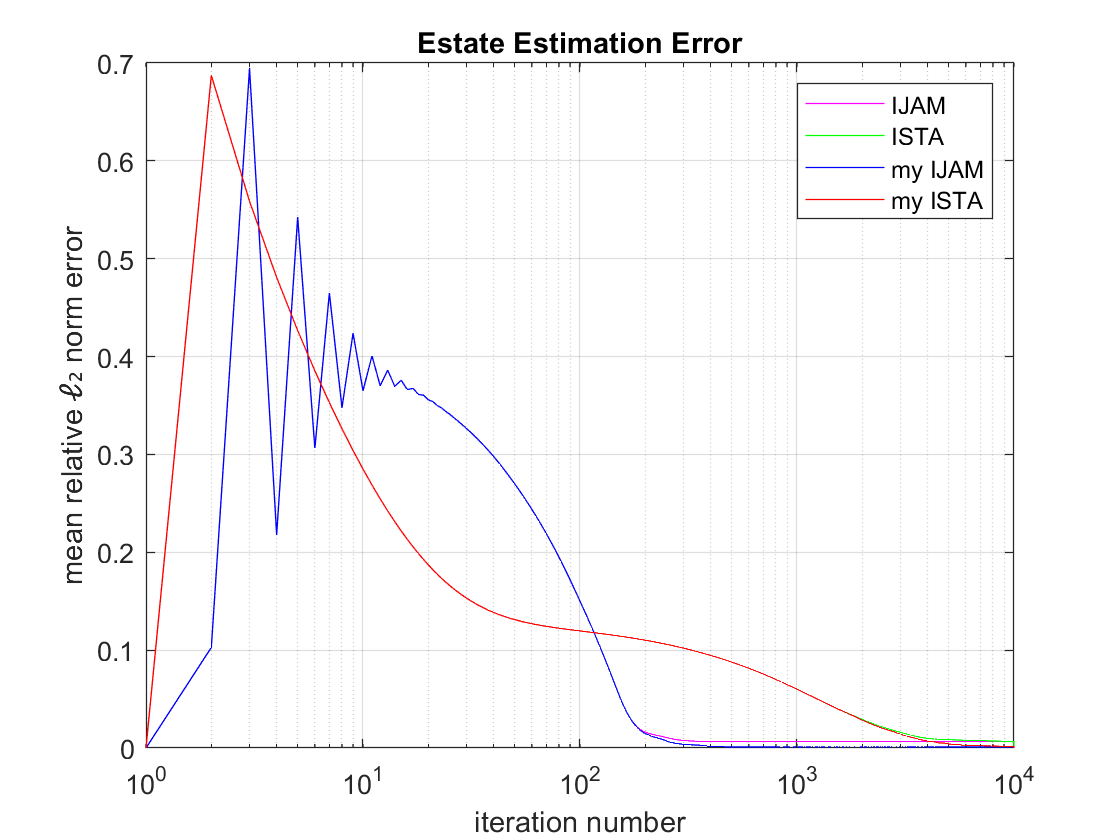
\includegraphics[width=0.75\textwidth]{mean_state_error.png} % Adjust width as needed
    \caption{Relative state error of the algorithms mention in the legend averaged in 20 run}
    \label{fig:example}
\end{figure}

\begin{figure}[H] % h means "here", can also use t (top), b (bottom), p (page)
    \centering
    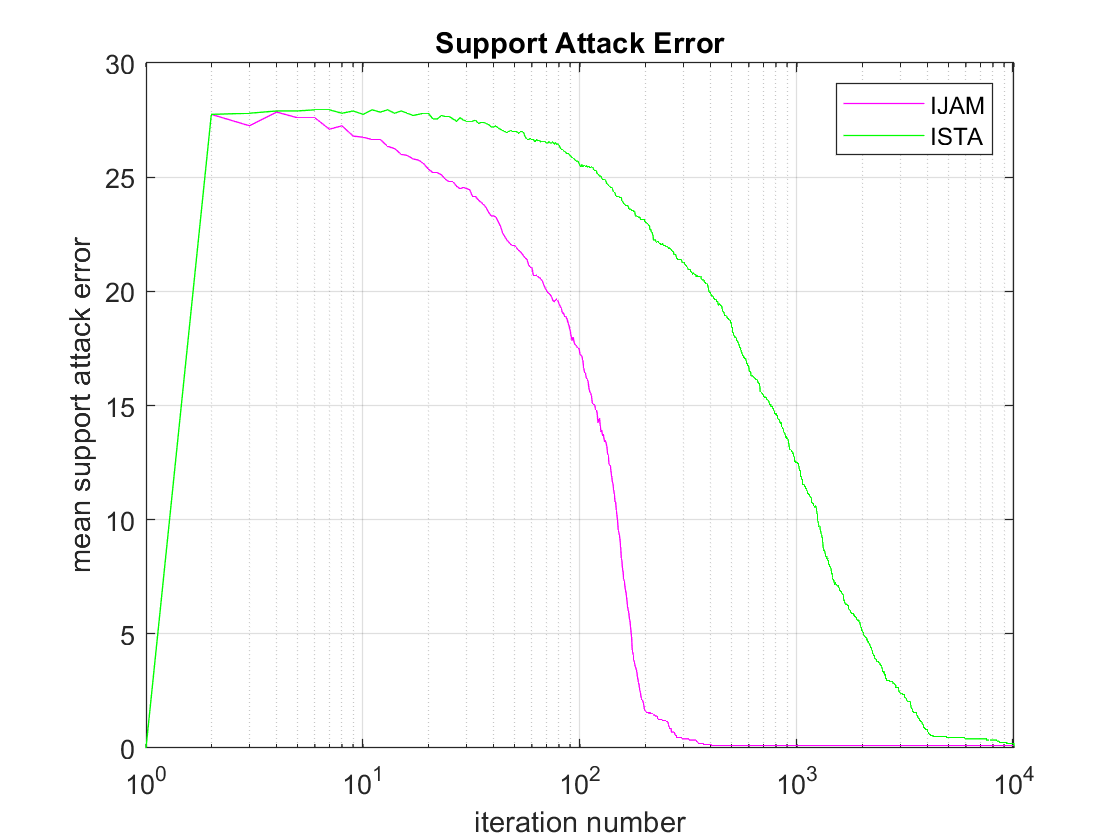
\includegraphics[width=0.75\textwidth]{mean_support_error.png} % Adjust width as needed
    \caption{Relative attack support error of the algorithms mention in the legend averaged in 20 run; my IJAM and my ISTA have the same performance as IJAM and ISTA, respectively.}
    \label{fig:example}
\end{figure}

\begin{figure}[H] % h means "here", can also use t (top), b (bottom), p (page)
    \centering
    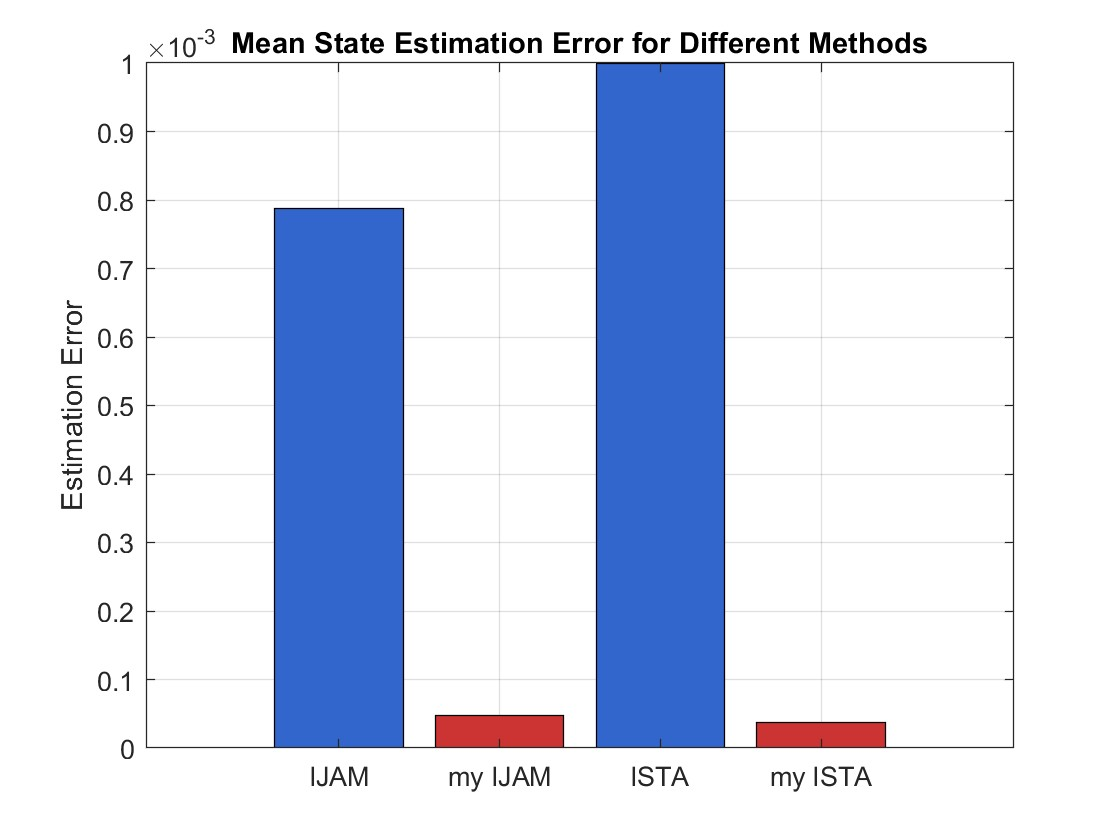
\includegraphics[width=0.65\textwidth]{precision_comparison.jpg} % Adjust width as needed
    \caption{comparison of the mean state error of the algorithms}
    \label{fig:example}
\end{figure}

Advantage of my ISTA, my IJAM, less average iteration, we don't need to estimate x to an exact precision, it is enough to find the position of the attacks, $90\%$ higher precision, since the problem is solved algabraically, we reach the global solution

\subsection{Tunning hyperparameters}
\subsubsection{changing $\lambda$}
$\lambda$ influence the weight of the first norm term in the partial lasso, which imposes sparcification. With large values of  $\lambda$, up to a certain extent, the convergence occurese in a less number of iterations, owing to the fact the soft-threshold pushed the values of attack vector to zero by a larger value. However, caution should be taken tuning lambda, since the larger value of $\lambda$ leads to over sparcification, which means underestimating small values of attack. This can be observed in the figures bellow where despide the fact that convergence occures in a less number of iterations for $lambda = 5$, but the algorithms cannot detect the position of the attack. On the other hand, if one sets the value of $lambda$ too small, other than leading to larger number of iterations, the algorithm considers noises and numberical inaccuracies as attack. 

\begin{figure}[H] % h means "here", can also use t (top), b (bottom), p (page)
    \centering
    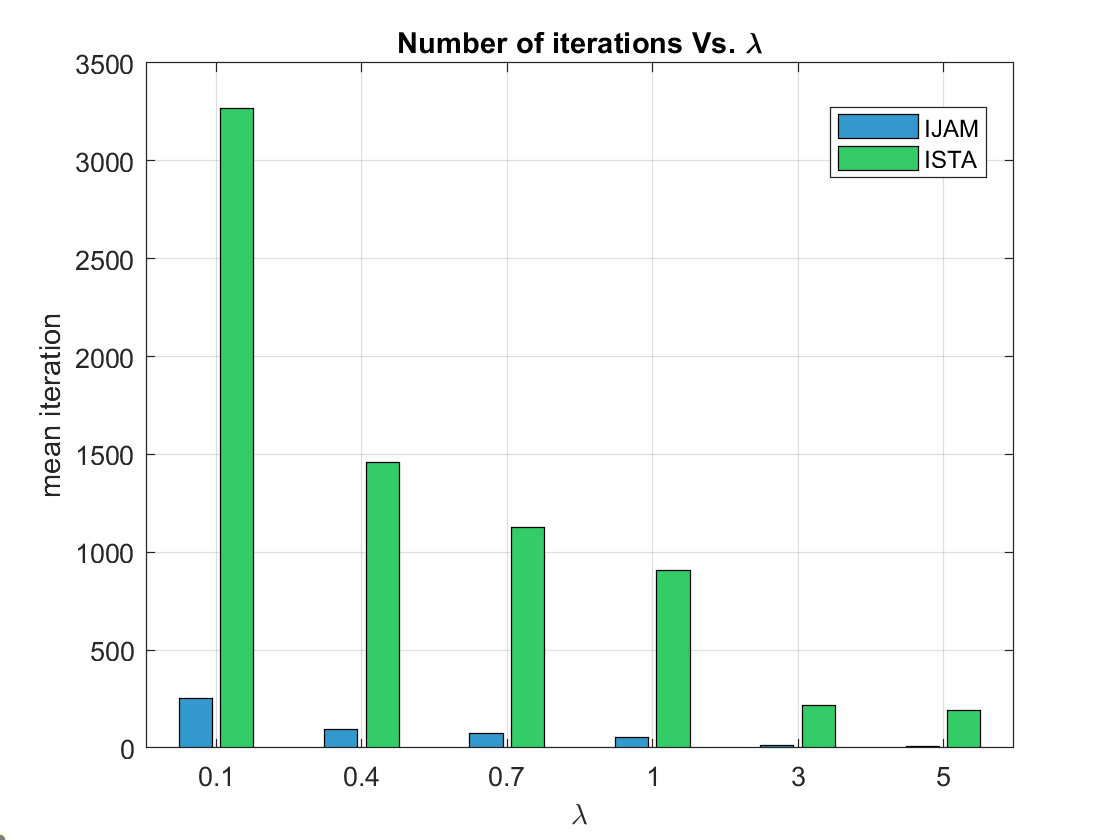
\includegraphics[width=0.65\textwidth]{iteration_vs_lambda.png} % Adjust width as needed
    \caption{Mean iteration required for convergance for different values of lambda}
    \label{fig:example}
\end{figure}

\begin{figure}[H] % h means "here", can also use t (top), b (bottom), p (page)
    \centering
    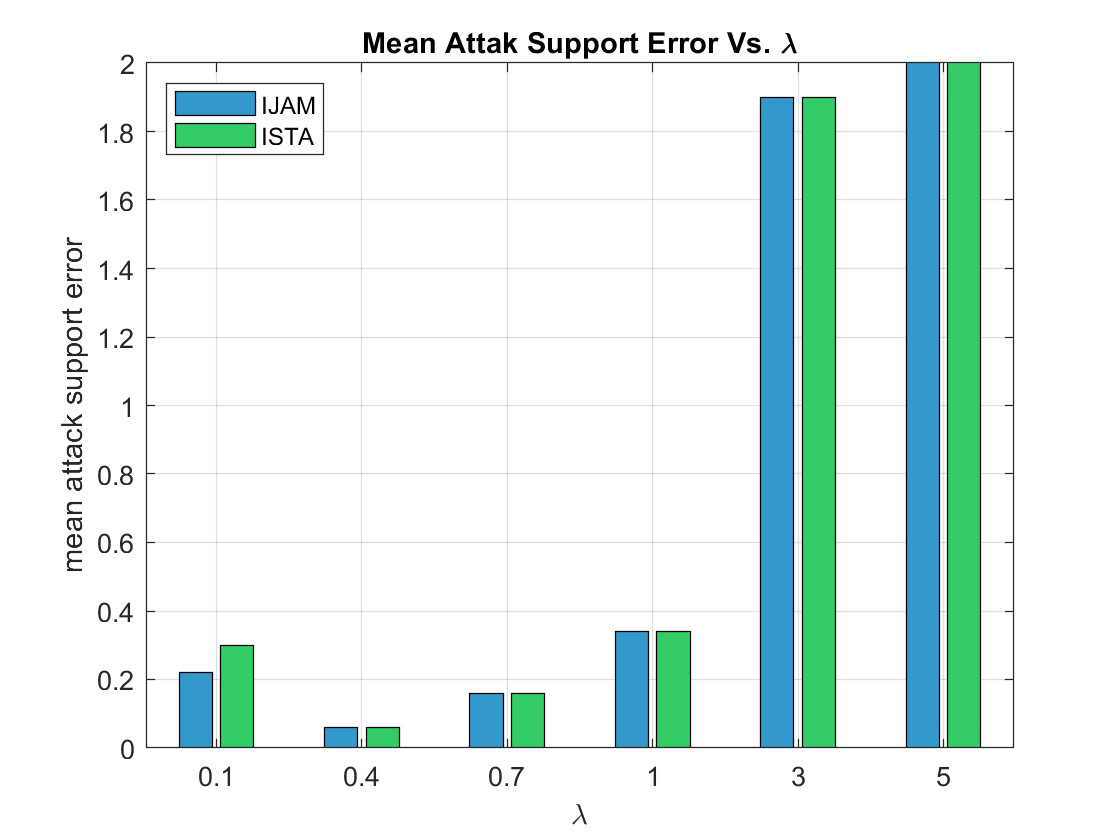
\includegraphics[width=0.65\textwidth]{attack_support_vs_lambda.png} % Adjust width as needed
    \caption{Mean attack support error of different methods for different values of lambda.}
    \label{fig:example}
\end{figure}


\subsubsection{changing $\nu$}
For the value of $\nu = 1$, we get the original algorithm for solving the problem; that is, no intertia is introduced in order to enhance the numerical stability of soft-thresholding operator, which is the case considering the state to be constant. However, for the range of  0 to 1, an inertia is introduced in the soft-thresholding. 

\begin{figure}[H] % h means "here", can also use t (top), b (bottom), p (page)
    \centering
    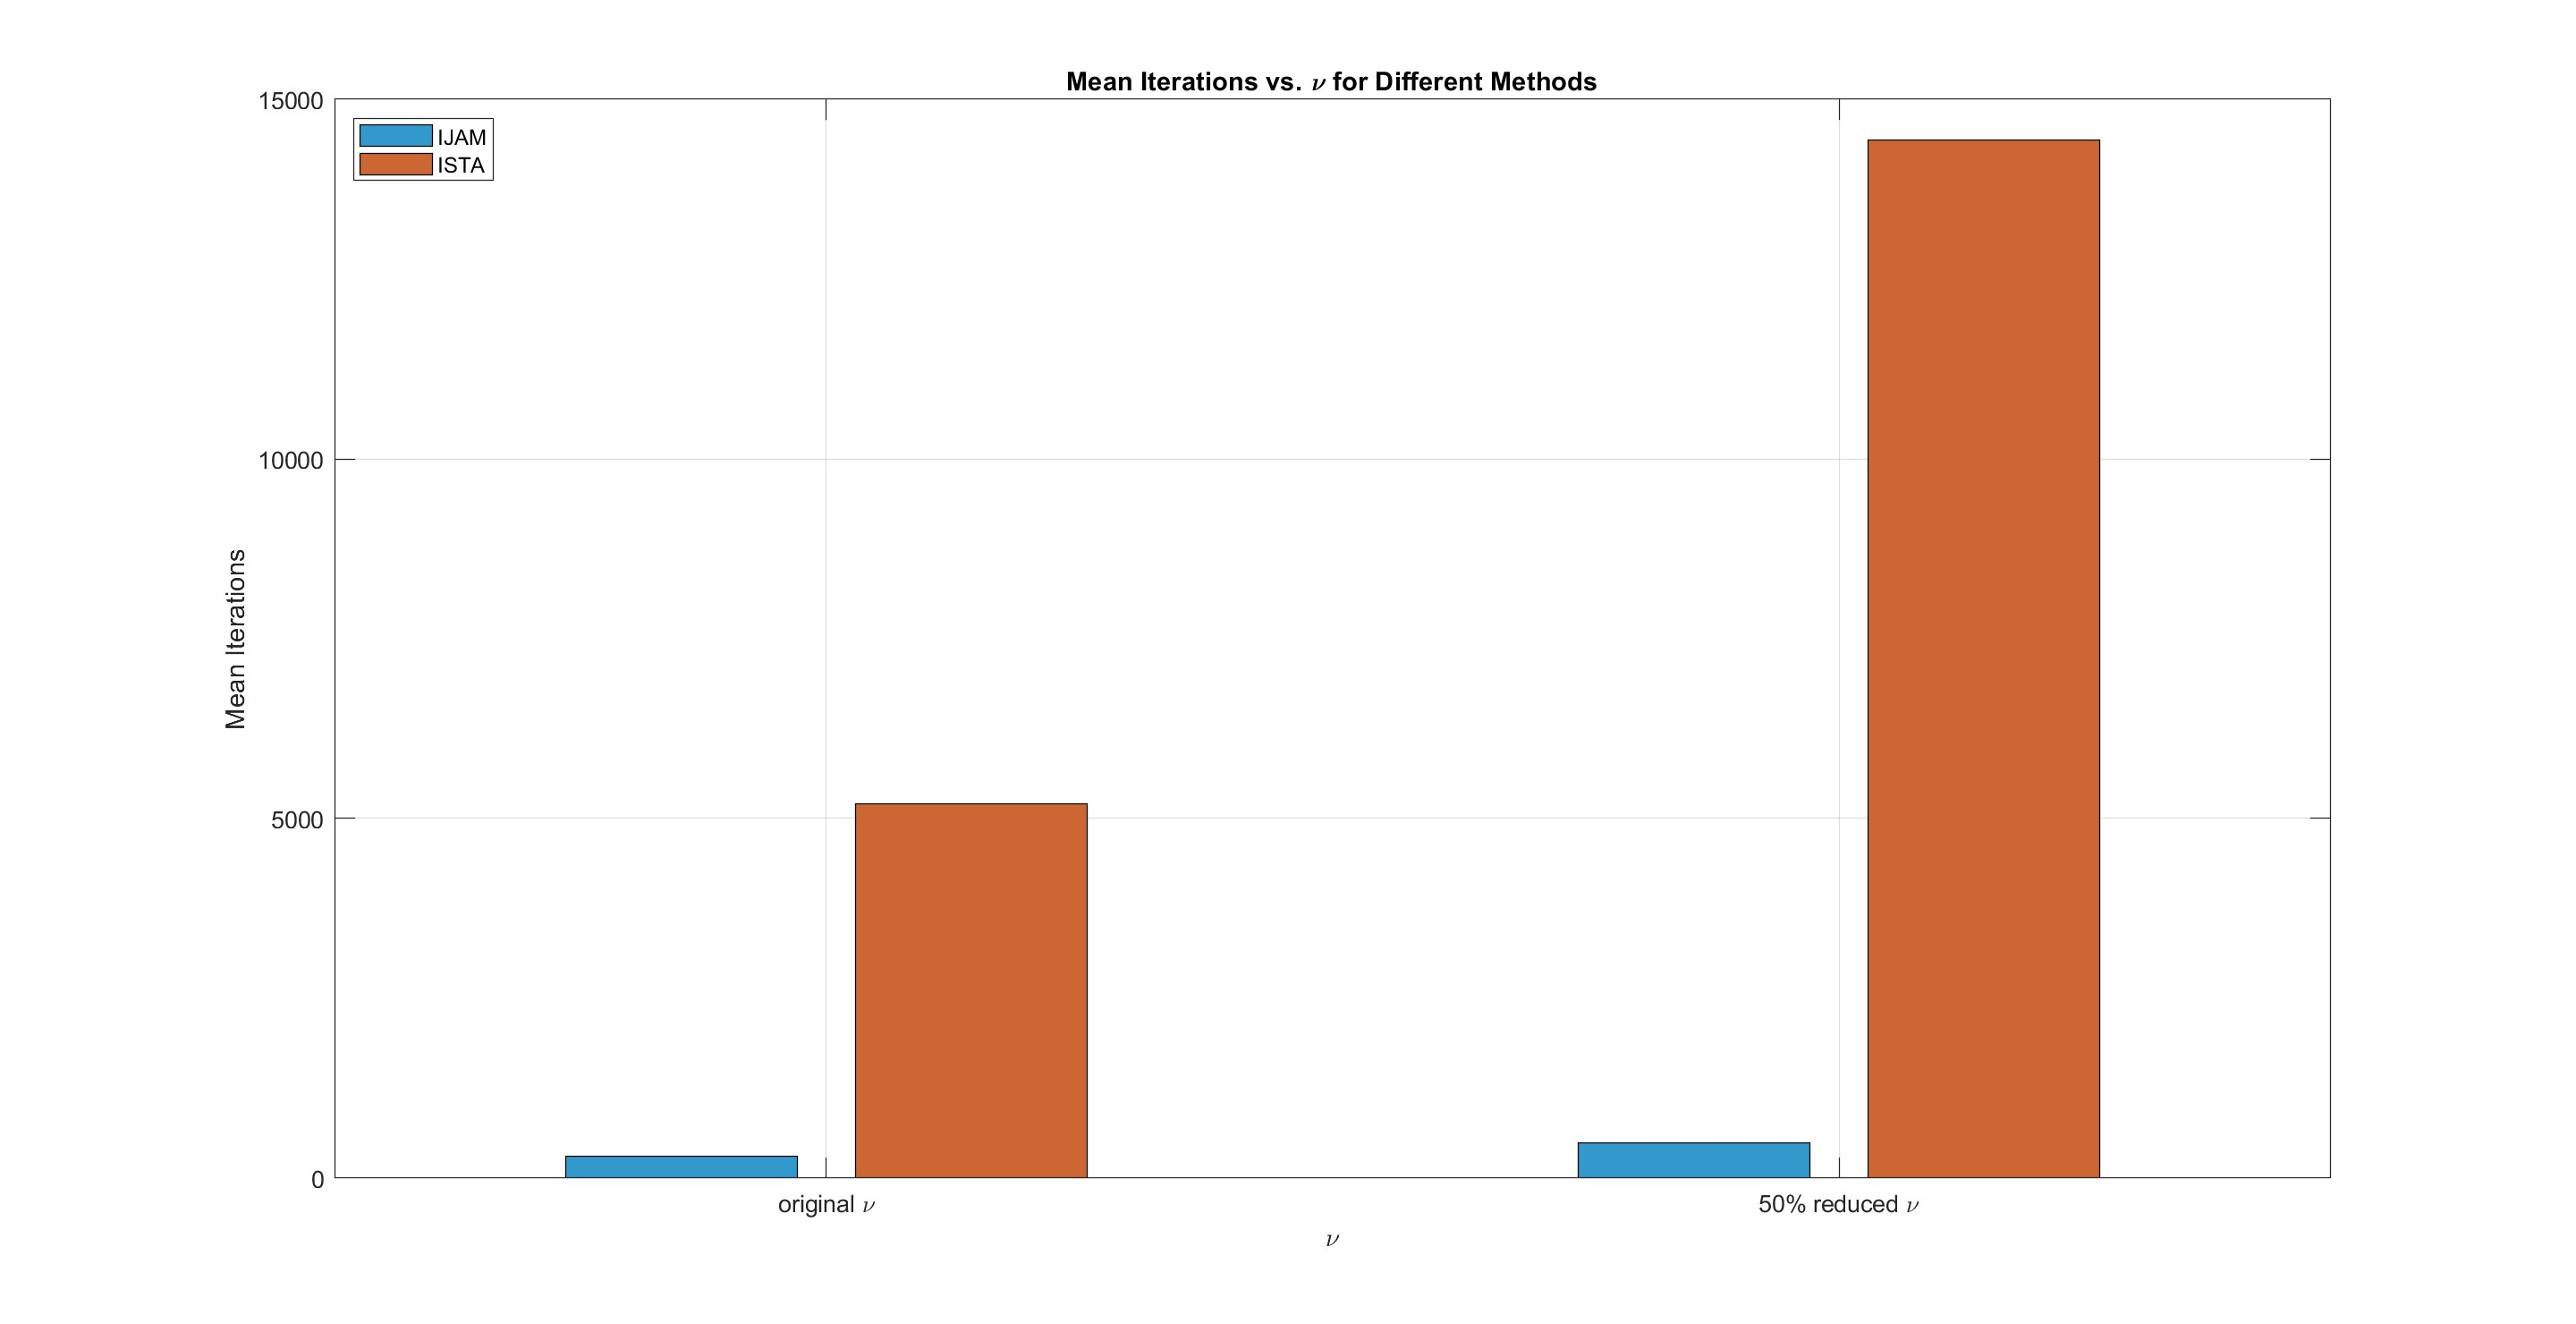
\includegraphics[width=0.65\textwidth]{iteration_vs_nu.jpg} % Adjust width as needed
    \caption{the plot of average number of iterations versus nu; the value of $\lambda$ is fixed to 1.}
    \label{fig:example}
\end{figure}

Having said that, for ISTA the value of the $\nu$ cannot be larger than a certain value; otherwise, the algorithm becomes numerically unstable. For ISTA, the Lipschitz condition ensures convergence by constraining 
\( \nu \) based on the spectral norm of \( C \):

\[
0 < \nu < \frac{2}{\|C\|^2}
\]

However, IJAM (Inertial Jacobi Alternating Minimization) is different because it does not use a direct gradient step for \( x \). Instead, it solves \( x \) via pseudo-inversion and applies an inertial term in the update for \( a \). This makes IJAM's convergence behavior less dependent on the Lipschitz constant and more on the inertia parameter \( \nu \) and the spectral properties of \( C \).

All in all, the optimal value of $\nu$ and $\lambda$ that guarantees a well performance cannot be introduced without a fixed $C$ matrix, which is the case while the algorithm were tested. Since ISTA and IJAM are used as the first step of ``my ISTA'' and ``my IJAM'', the same arguments holds for those two.

\subsubsection{Resilience to the number of the attacks}
Considering the dimension of the matrix $C$, the following necessary condition holds, intorducing the maximum possible number of the attacks that can be corrected:
\begin{equation}
h \leq \frac{q - n -1}{2}
\end{equation}
Considering the dimension of our problem:
\[
h \leq 7
\]

and there is proven another theory mentioning that $h$ errors are correctable if and only if:
\begin{equation}
\forall x \in \mathbb{R}^n, \ \|Cx\|_0 \geq 2h + 1
\end{equation}

However, not knowing $C$ this analize cannot be done, since we don't have any information about the dimension of the null space of $C$.

\begin{figure}[H] % h means "here", can also use t (top), b (bottom), p (page)
    \centering
    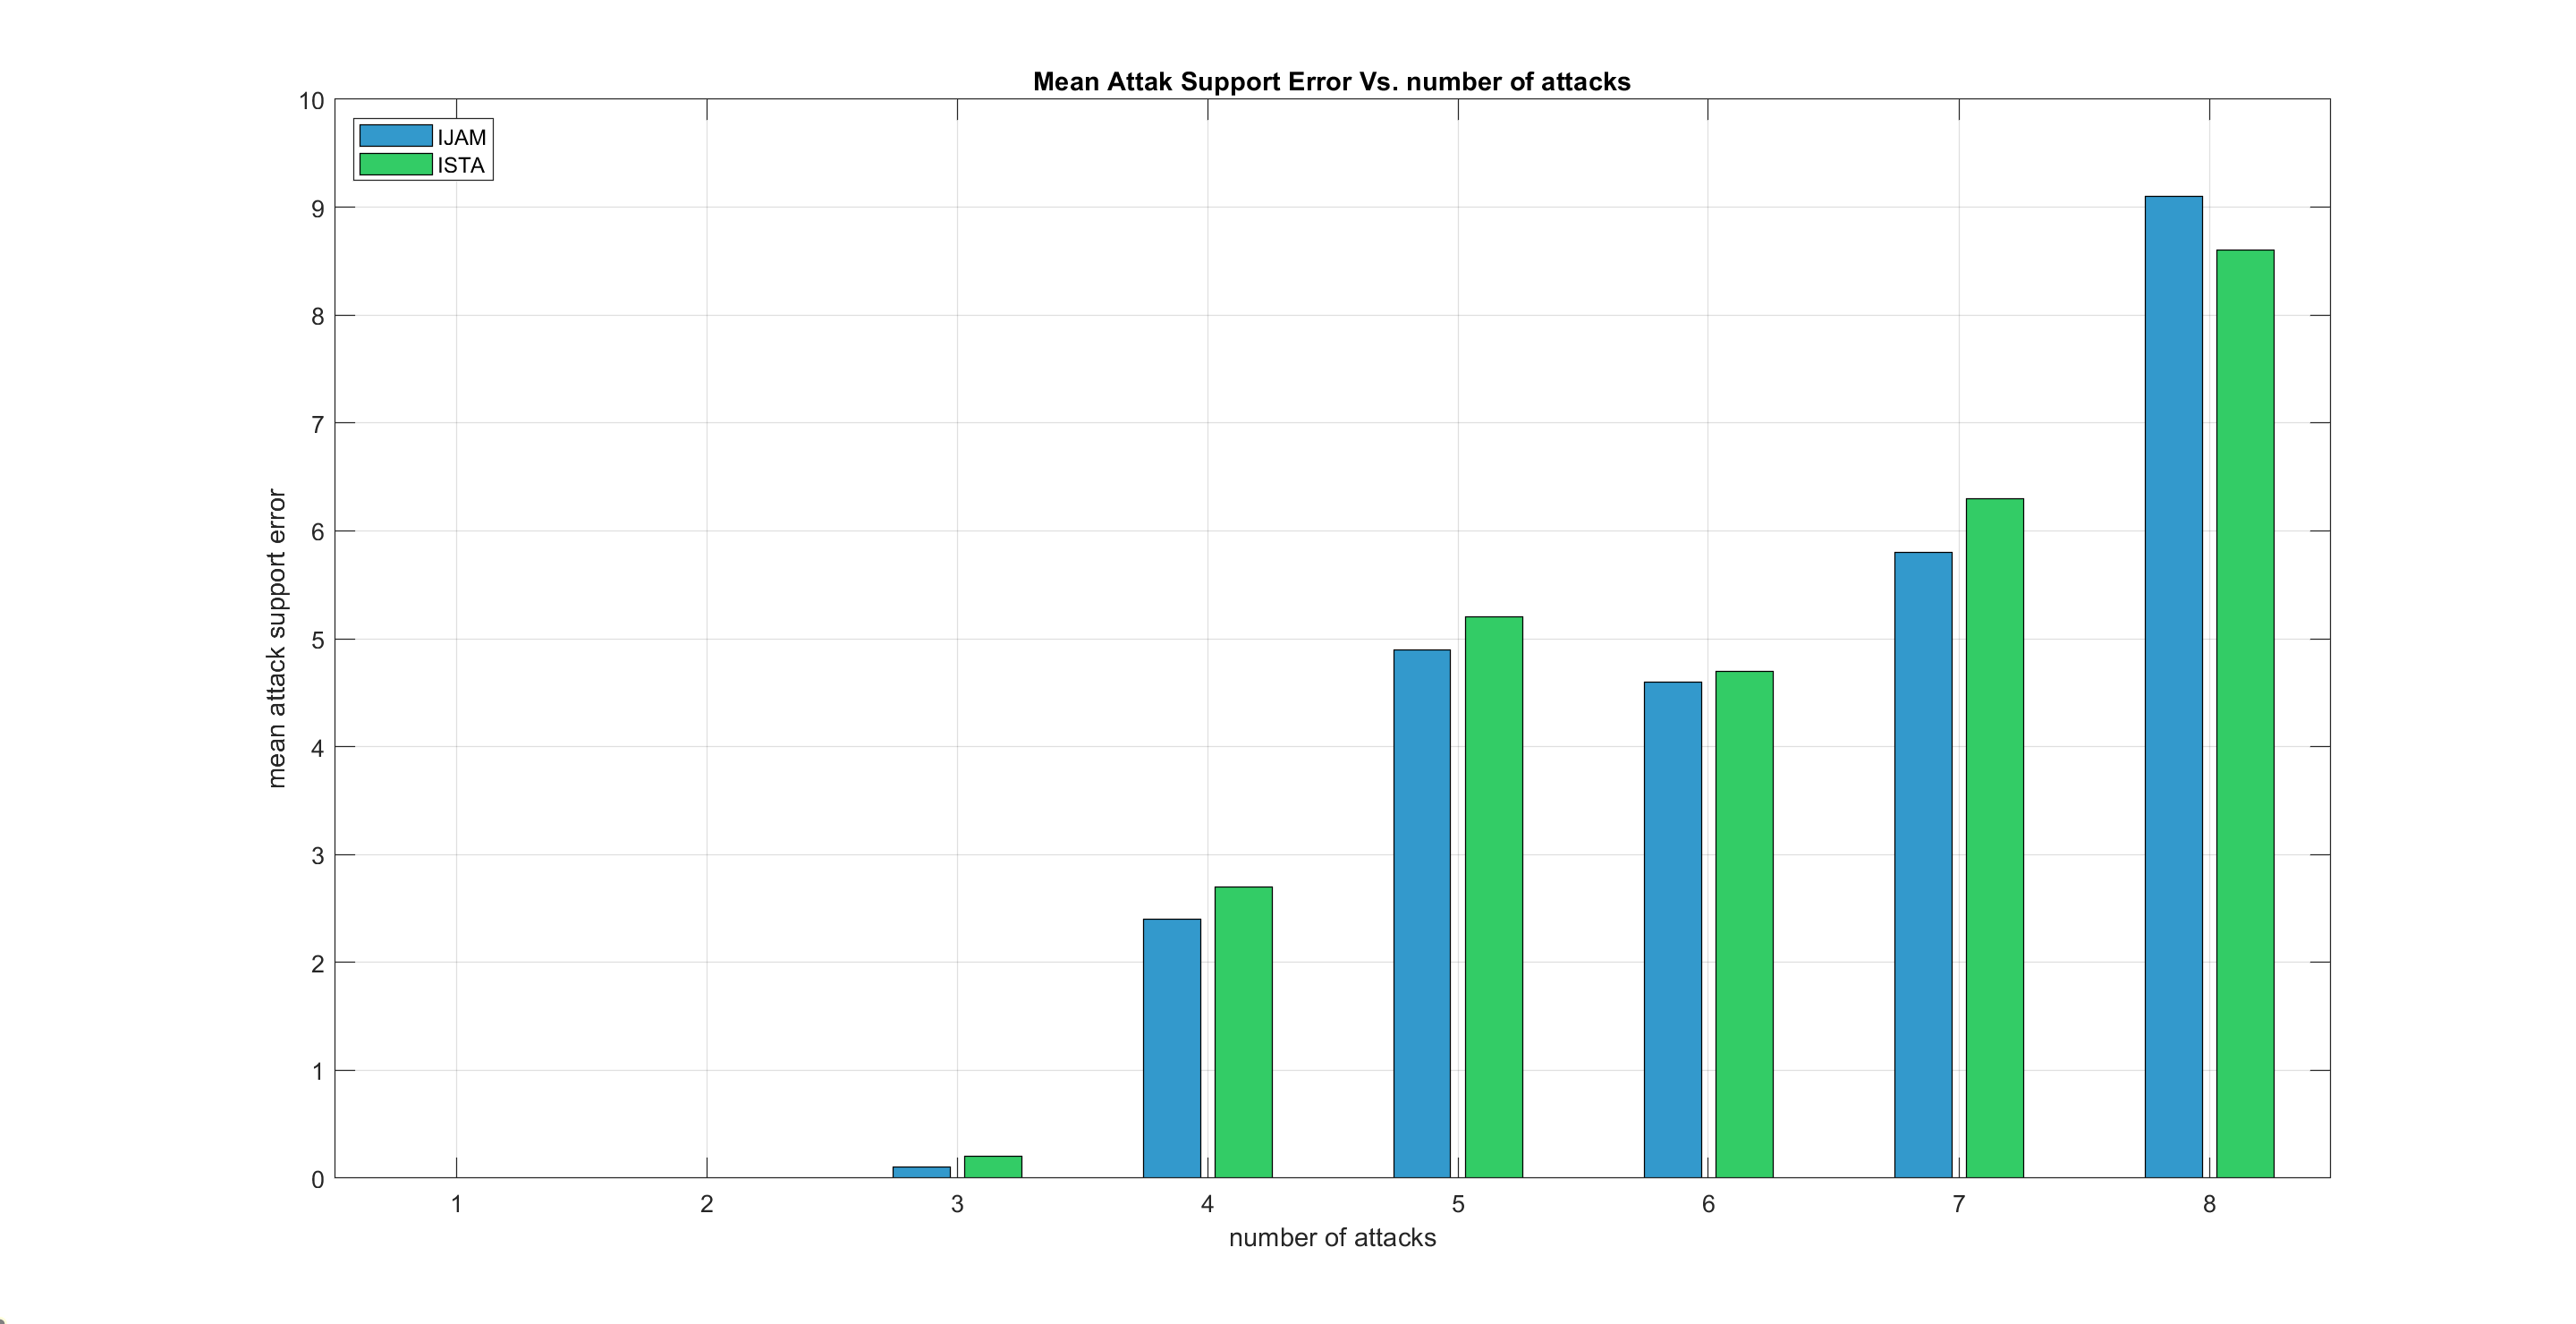
\includegraphics[width=0.75\textwidth]{resilience.png} % Adjust width as needed
    \caption{Mean attack support error in 20 run for different number of attacks.}
    \label{fig:example}
\end{figure}

It can be seen that by the time the number of attacks passes 7, almost all the time, the algorithm cannot detect the position of the attacks, supporting the theory regarding the number of correctable attack.
\section{Further Discussion}
\subsection{My Conjecture}
The position of the h-sparse attack can be found solely by solving the least-squares problem. Having solved the following least-squares problem:
\begin{equation}
    z = (C, I)^{+} y
\end{equation}
where
\begin{equation}
    z = 
    \begin{bmatrix}
        x \\
        a
    \end{bmatrix}
\end{equation}
a diagonal \( q \times q \) attack support matrix, \( M_a \), can be shaped which has 1 corresponding to the \( h \) components of \( a \), such that:
\begin{equation}
    z = G_{\text{sparse}}^{+} y
\end{equation}
where
 \begin{equation}
    G_{\text{sparse}} = 
    \begin{bmatrix}
        C M_a
    \end{bmatrix}
\end{equation} 

For $h = 1$, this method detect the correct position of the attack 80 percent of the time, without any iteration and just by two times solving a least-square problem! However, with $h = 2$ this number reduces to almost 50 percent of the time. In my opinion, this is more than a lucky guess and there must be a simple way using least square algorithm combined with some property of $C$ or some geometrical intrepretaiton, in order to find the position of the attacks.
\subsection{The energy of the attack}
If the energy of the attacks is considerable compared to the energy of the measurement vector Cx the aboved mentioned method can easily identify the attacks:
As an instance, the matrix \texttt{C = 0.01*randn(q,n)} is considered, while the value of the attack is kept constant. In this case, the attacks can be found up to a large number and with a good precision. The result can be seen in the following graphs.
\begin{figure}[H] % h means "here", can also use t (top), b (bottom), p (page)
    \centering
    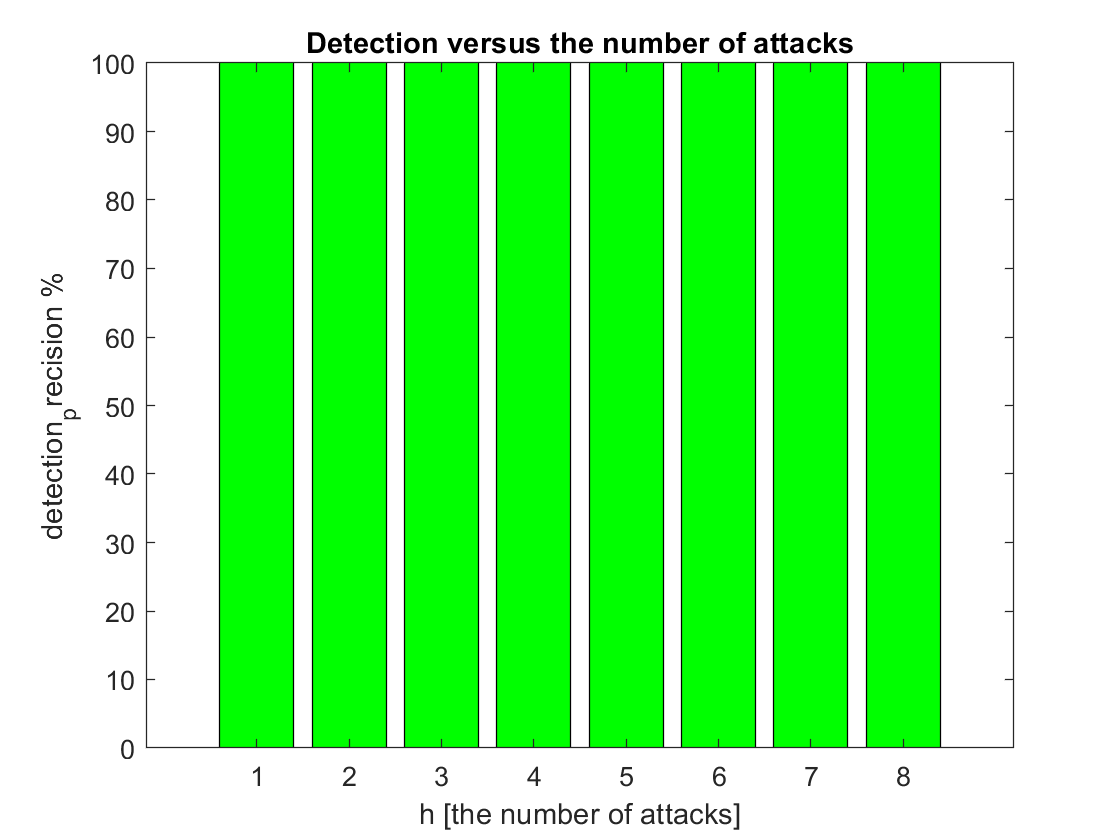
\includegraphics[width=0.65\textwidth]{detection_precision.png} % Adjust width as needed
    \caption{Detection versus the number of attacks}
    \label{fig:example}
\end{figure}

\begin{figure}[H] % h means "here", can also use t (top), b (bottom), p (page)
    \centering
    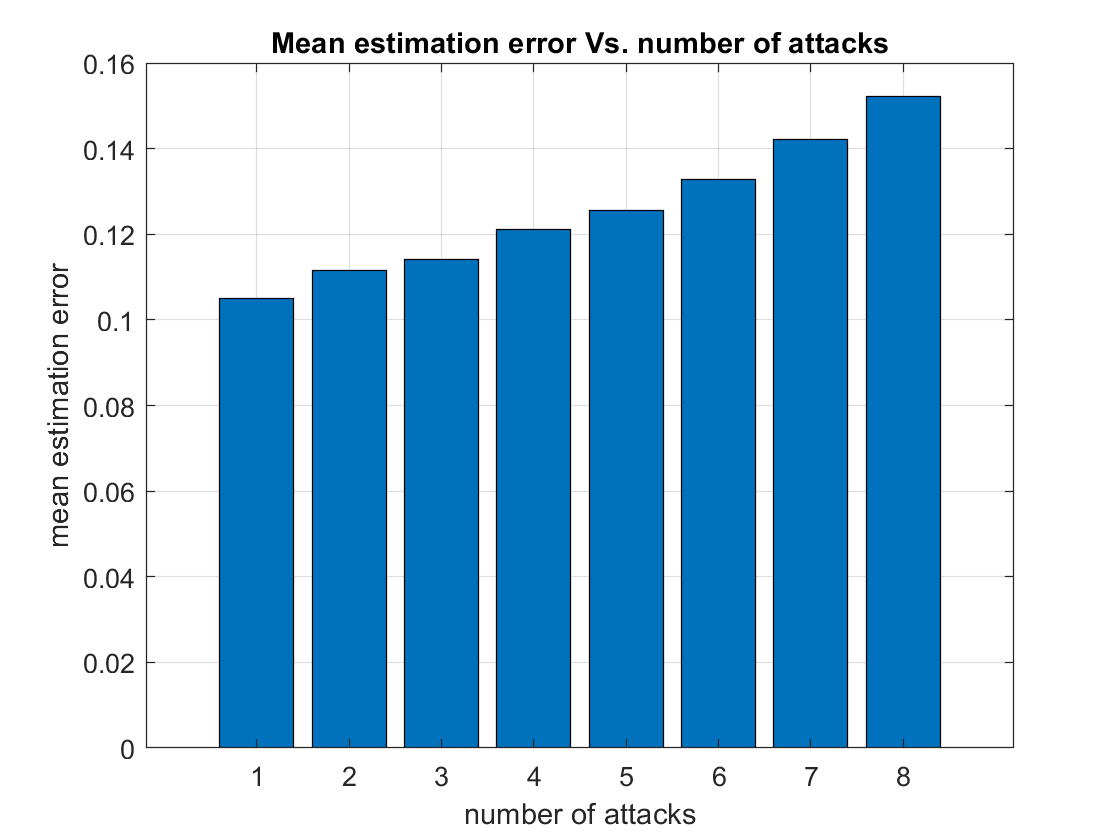
\includegraphics[width=0.65\textwidth]{mean_see.png} % Adjust width as needed
    \caption{Mean estimation error over; 1000 run for each number of attacks}
    \label{fig:example}
\end{figure}


\section{Conclusion}
It was observed that both IJAM and ISTA, are capable of detecting and correcting the effect of the attack by setting correctly the values of the hyper parameters. 

Regarding the precision of the algorithms, it was observed that my IJAM and my ISTA enjoy a higher precision compare to IJAM and ISTA, due to the fact that they almost reach the optimal solution of least-square algorithm. Nonetheless, still these two algorithms depend on IJAM and ISTA, in order to detect the position of the attacks.

 Regarding the hyperparameters, larger values of $\lambda$ leads to a faster convergence of the algorithm; however, in this case, the algorithms may overlook attacks with values smaller than $\lambda$. On the other hand, if $\lambda$ is selected too small, the algorithm considers noises and numerical inaccuracies as attack components. As to $\nu$, the numerical stability of the algorithms depends on this value, as it endows a sort of ``numerical inertia'' to the algorithms. Especially, ISTA is more dependent on this value as it uses gradient decent for converging to the estimation of the state vector, and for value of $\nu$ larger than Lipschitz condition, the algorithm becomes unstable. Stability of IJAM is less dependent on this value, but still the value of $\nu$ helps the stability of attack detection, since still a gradient decent is happening at each iteration for converging to the estimation of attack values.
 
Regarding relisience of the algorithms, considering the number of the states and the number of our sensors, thoretically, the algorithms cannot detect more than 7 number of attack. It was also observed that the attack support error grows as the number of attacks increases. In large scale systems, assuming that the number of attacks are small, these algorithms can be effective.
 
 












% !TeX root = ../main.tex
\chapter{Project 02: Target localization under sparse sensor attacks}

\section{Objectives}
The aim of this project is to localize the position of a device using RSS fingerprinting setting. In this project, we are given the dictionary $D$, and it is requested to localize the position of the device having a given measurement.

\section{Setting of the problem}
The localization problem is set in 10 by 10 squaremeters room. The room is gridded into 100 cells and 20 sensors are used in the training phase. In addition, it is assumed that during the training step has done in an offline manner, and therefore, the dictionary $D$ is assumed to be attack free. During the ``routine'' phase, which it is required to locate the position of the device, it is considered that 5 sensors are under attack, and the task is to localize the position of 1 target in this room given a vector of measurements. Therefore, the dimensions of the problem are as follows:
\begin{figure}[H] % h means "here", can also use t (top), b (bottom), p (page)
    \centering
    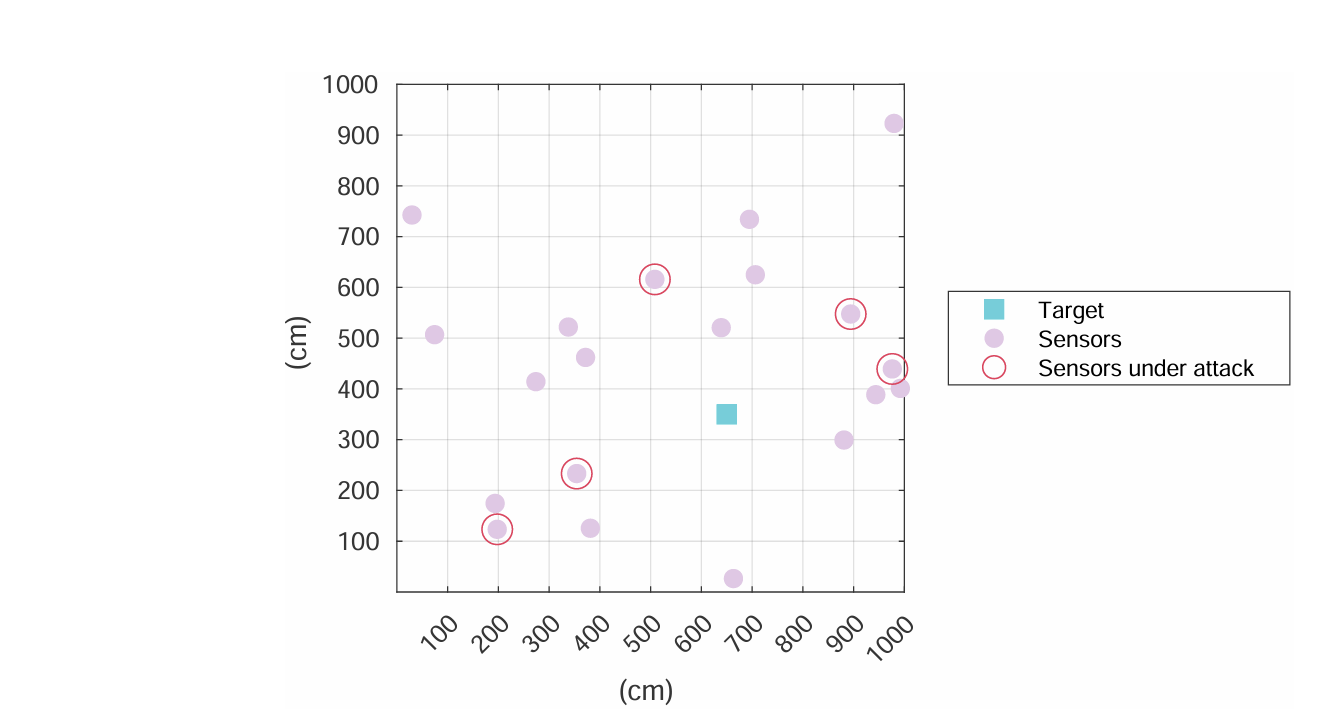
\includegraphics[width=0.75\textwidth]{localization_setting.png} % Adjust width as needed
    \caption{The graphical setting of the problem; reported from the project 2025 file.}
\end{figure}
\begin{itemize}
	\item the number of the cells (states) $n = 100$,  states can be 0 or 1, and only 1 state can be 1.
	\item the number of the sensors, length of the measurement sensor $q = 20$
	\item the number of the attacks $h = 5$
\end{itemize}

The same as the previous project, the problem to be solved is sparse. The diffence is that this time both the state vector and the attack vectors are expected to be sparse. Hence, a full weighted Lasso needs to be considered:

\begin{equation}
\min_{x \in \mathbb{R}^{n}, a \in \mathbb{R}^{q}} \left\| G \begin{pmatrix} x \\ a \end{pmatrix} - y \right\|_2^2 + \lambda_1 \| x \|_1 + \lambda_2 \| a \|_1
\end{equation}
where,
\[
G = (D, I)
\]

Here, in order not to face numerical problems, G should be normalized, this is done using \texttt{normalize( )} command in MATLAB. In this way, we make sure that $G$ and $I$ are of the same scale.

\section{Implementation of the algorithm}
The iterative algorithm used in order to converge to the solution of weighted Lasso is simular to the one implemented in the first project, with the difference that, since we know here also the state vector is going to be sparse, the soft-thresholding is used both for the attack and state vectors. Hence, after the initialization of the state and attack vectors, the following algorithm is implemented:

\begin{equation}
\begin{pmatrix}
x(k+1) \\
a(k+1)
\end{pmatrix}
=
\mathcal{S}_{\nu \lambda} \left[
\begin{pmatrix}
x(k) \\
a(k)
\end{pmatrix}
- \nu G^\top \left(
G \begin{pmatrix}
x(k) \\
a(k)
\end{pmatrix}
- y
\right)
\right]
\end{equation}

The suggested parameters for this problem is:
\begin{itemize}
	\item $\lambda_1 = \lambda_2 = 10$
	\item $\nu = \|G\|_2^2$
\end{itemize}

This algorithm is run until the difference of the two consequitive states becomes lower that $\delta = 10^{-10}$.

Once this goal is achieved, the state position needs to be cleaned. That is, 0 should be allocated to the states with values smaller than a certain threshold, and 1 should be allocated otherwise. In the given problem, it cannot be expected that, after performing cleaning, the state vector have more than one non-zero component - having only one target. At the end of  this step, both the position of the target and the position of the attacks are estimated, given the sensor measurements.

In order to estimate the correct values of attack, a support matrix corresponding the position of the attacks needs to be shaped. Then, the correct value of the attacks can be calculated as follows:

\begin{equation}
	\hat{a} = S_a^{+} \left( y - D \hat{x}_{cleaned}\right)
\end{equation}

In an attemp to enhance the performance of the algorithm the following values were used as hyperparameters:
\begin{itemize}
	\item $\nu = 0.0033$
	\item $\lambda_1 = 14$
	\item $\lambda_2 = 11.4$
\end{itemize}


\section{Results,}
Having run the algorithms for both suggested and enhance hyperparameters, the following table was obtained.

\begin{table}[ht]
\centering
\begin{tabular}{|c|c|c|c|}
\hline
\textbf{items} & \textbf{Real Data} & \textbf{suggested parameters} & \textbf{enhanced parameters} \\ \hline
\textbf{Iteration} & **** & 3752 & 1358 \\ \hline
\textbf{Attack Position} & \{1, 10, 14, 16, 17\} & \{1, 10, 14, 16, 17\} & \{1, 10, 14, 16, 17\} \\ \hline
\textbf{Target Position} & cell 37 & cell 37 & cell 37 \\ \hline
\end{tabular}
\caption{The results of running the algorithm with suggested and enhanced hyperparameters}
\end{table}

The estimated values of the attack are as follows:

\begin{figure}[H] % h means "here", can also use t (top), b (bottom), p (page)
    \centering
    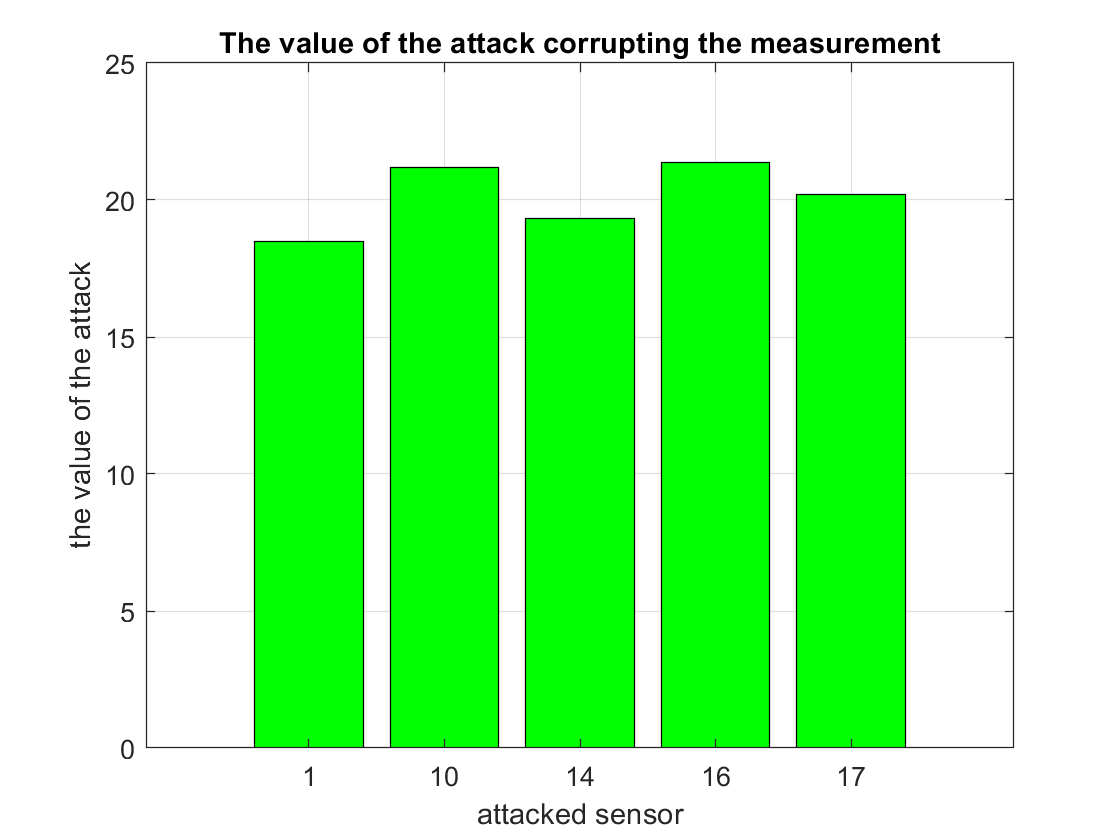
\includegraphics[width=0.5\textwidth]{attack_values.png} % Adjust width as needed
    \caption{The bar plot of the value of the attacks corrupting the sensors}
\end{figure}

\section{Further discussion: }
\subsection{why not IJAM?}
Regardless of the dimension of the problem, IJAM ``aggressive'' transient combined with soft-thresholding does not result in a good performance, since in the iterations where the value of the states drops suddenly, the soft-thresholding cuts those value. If the number of sensors are more than the number of cell the following steps can be followed:

\begin{enumerate}
	\item Having a transient phase where soft-thresholding is not applied to the state and we weight so that the transient passes. This can be coded by setting a threshold to check the difference in two consequetive state update is lower than a certain value.
	\item Then, we include soft-thresholding also for the state.
\end{enumerate}

However, in the problem at hand, the number of sensors are less than the number of cells and intrinsically underdetermined, and solving the problem with the psuedo inverse does not lead to an absolute minimum. 

\subsection{finding the position of the sensor}
Having the matrix $D$, the position of the sensors can be easily find. As each row of $D$ includes the signal strength of target in different cells, it is reasonable that the maximum element of each row, corresponds the cell that the signal is closer to, and therefore, the position of the sensor. The position of the sensors obtained are as follows:

\begin{table}[ht]
\centering
\caption{The number of the cell in which each sensor is places.}
\label{tab:sensor_positions}
\begin{tabular}{cc|cc}
\hline
\textbf{Sensor \#} & \textbf{Position} & \textbf{Sensor \#} & \textbf{Position} \\ \hline
1  & 66  & 11 & 54  \\
2  & 77  & 12 & 71  \\
3  & 43  & 13 & 44  \\
4  & 14  & 14 & 12  \\
5  & 7   & 15 & 50  \\
6  & 51  & 16 & 59  \\
7  & 29  & 17 & 24  \\
8  & 40  & 18 & 57  \\
9  & 68  & 19 & 12  \\
10 & 50  & 20 & 100 \\ \hline
\end{tabular}
\end{table}

The grafical representation of the sensors in the room can be compared to the actual setting in the following plot.

\begin{figure}[H]
    \centering
    \subfloat[The number of sensors in each cell]{
        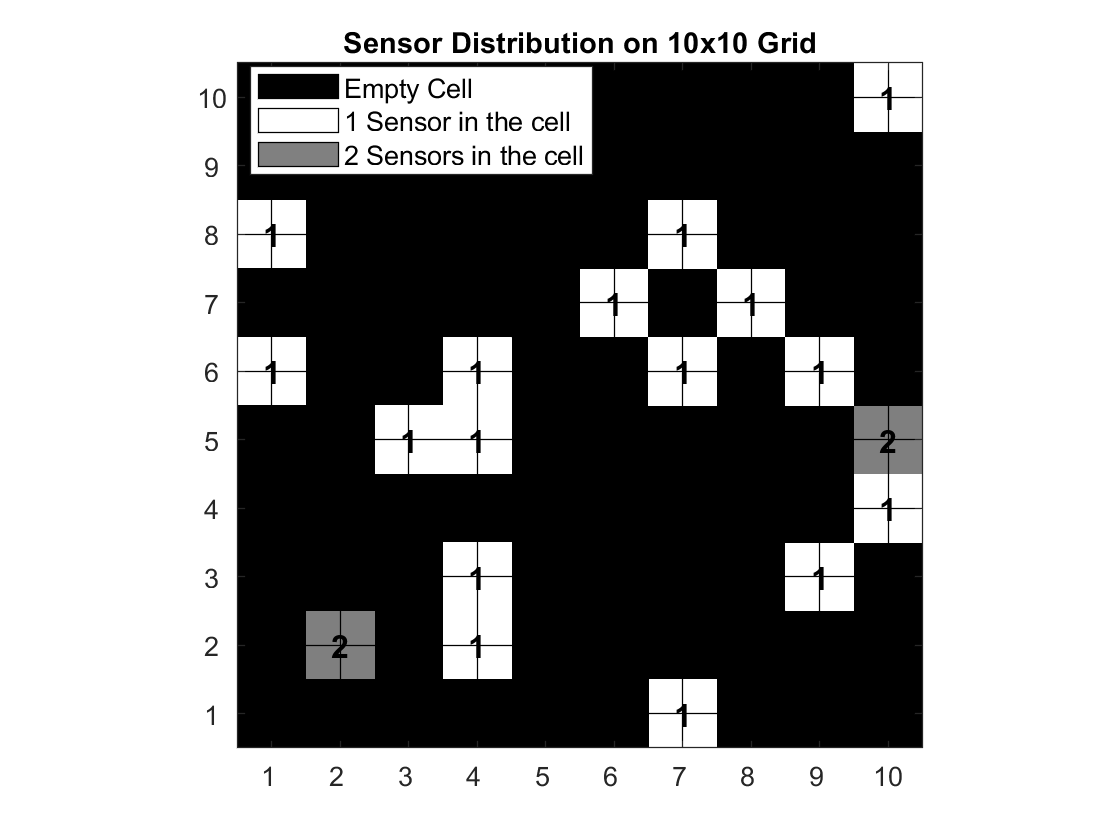
\includegraphics[width=0.35\textwidth]{sensor_position.png} % Adjust width as needed
    }
    \hspace{1cm} % Adjust the space between the two figures
    \subfloat[The head map of the attack support vector of different nodes after the consensus in the Star topology.]{
        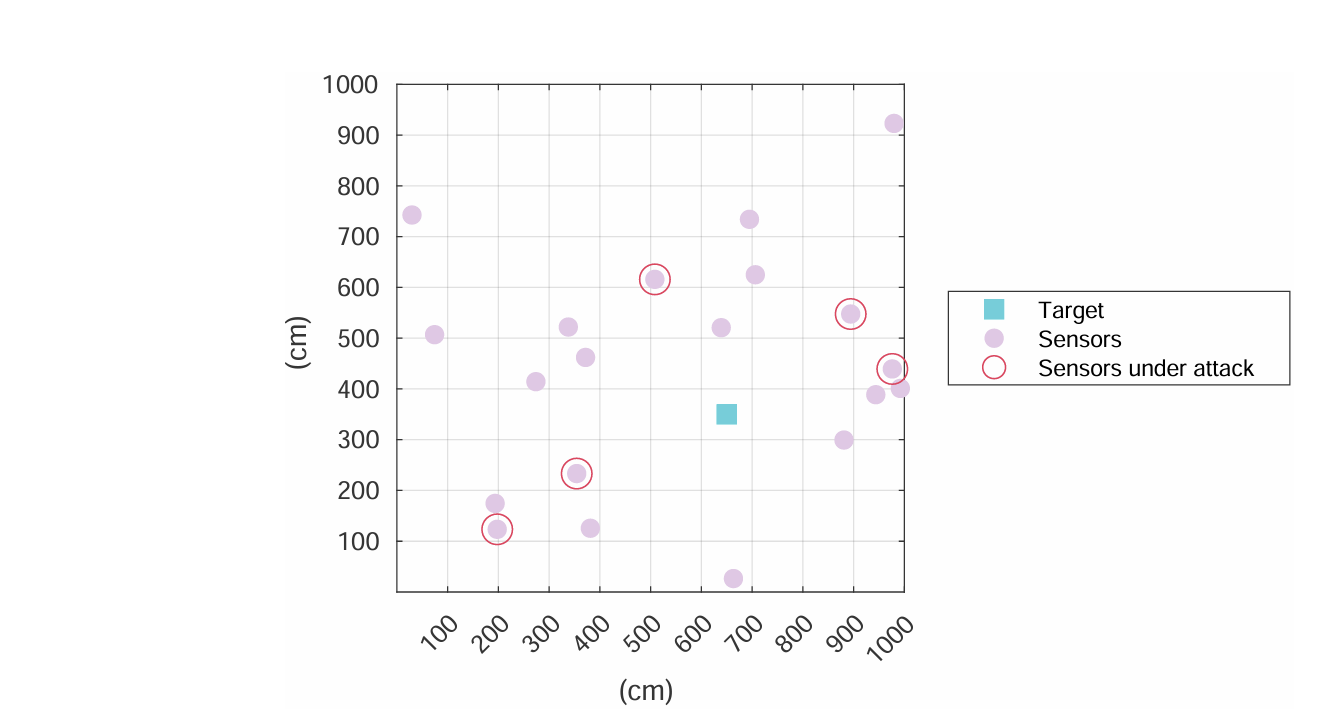
\includegraphics[width=0.55\textwidth]{localization_setting.png} % Adjust width as needed
    }
    \caption{The real and the estimated position of the sensors under attack.}
\end{figure}

\subsection{Localization using 1 attack-free sensors and not 3. How is it possible?}
From geometrical point of view, 3 sensors should be adopted in order to obtain a unique point in a plane. However, during the dictionary shaping, the center of the cells are used for placing the target, and the sensors are placed near the boarder of the cells. For this reason, considering any given cell and any given sensors, the arc that passes from the center of the cell does not passes the center of another cell, and thereby the measurement of target signal from the center of any cell would not be exactly the same as the measurements taken from the center of another cell, even if geometrically they both approximately have the same distance from the sensor. All in all, one attack-free, precise-enough sensor must be enough so as to locate the position of the target placed at the center of cells. In our case, using the sensor number 5, 6, 7, 11, 18, and 19 the position of the target was located in the following manner.

\texttt{[\~ \,, position] = min(D(sensorNumber,:) - y(sensorNumber))}

In our case, one cannot be sure whether the measurements are accurate enough to lead to the same result for measurement of other cell. Then, taking the effect of noises in to account, two sensors may be adopted for doing so.

\texttt{[\~ \,, position] = min(vecnorm(D([2, 3],:) - y(2:3),2,1))}

This was perfromed with some other 2 pairs of sensors, and the correct result was obtained each time. 


\section{Conclusion}
It can be seen that ISTA algorithm converges to the solution of weighted Lasso, and can correctly detect the position of the target as well as the position of the attacks sensors and the value of the attack. It was observed that the enhanced hyperparameter values led to a convergence rate that was twice as fast as the suggested values.

Since IJAM does not enjoy a smooth transient, the introduction of soft-thresholding disrupts converging to the solution of the problem. However, it is proposed a two step algorithm for implementing IJAM: 1) running normal IJAM so that the transient passes without applying soft-thresholding to the states, 2) applying soft-thresholding also to the states.

Having the matrix D, the position of sensors can be easily found, thanks to the fact that given a constant sensor, or at any rate row of the matrix D, the highest value correspond to the cell where that sensor is closer too, and hence the position of the sensor.

Further, it was observed that using 1 attack-free, precise sensor, the position of the target can be located in a plane. Nonetheless, to take in to considerations the effect of measurement noise, 2 sensor can be adopted for doing so, still the number of sensors adopted are lower than geometrical intuition suggest for localization in a plane.









% !TeX root = ../main.tex
\chapter{Project 03: Secure State Estimation of a Dynamic CPS with Sparse Sensor Attacks}

\section{Objectives}
The aim of this project is to use an online observer in order to estimate the state of the given system un sensor attack, which entitles estimating the states and the attacks at the same time.

\section{Setting of the problem}
The system provided for performing this task is an autonomous LTI system with the following state space representation:

\begin{equation}
	\begin{cases}
		x(k+1) = A x(k) \\
		y(k) = C x(k) + a
	\end{cases}
\end{equation}
where,
\begin{itemize}
	\item the state dimension is $n = 15$
	\item the number of sesors is $q = 30$
	\item the number of sensor under attack $h = 3$
\end{itemize}

It is assumed that attack is going to remain constant for a time-windows, which can be a reasonable assumption having an small enough sampling rate.

\section{Implementation}
\subsection{Luenberg Observer}
The system under the study has a mode equal to 1. According to the proposition of Observability of Dynamic CPSs with constant attacks, If the matrix $A$ has an eigenvalue equal to 1, the dynamic CPS with constant attacks is not observable. Hence, we cannot adopt a Luenberg observer.

\subsection{Sparse Soft Observer (SSO)}
This observer, which is the dynamical version of the ISTA can be adopted in order to perform online secure estimation for a dynamical system. The steps of these iterative algorithm is as follows:

\textbf{Initialization:} \(\tau > 0\), \(\hat{x}(0) \in \mathbb{R}^{n}\), \(\hat{a}(0) \in \mathbb{R}^{q}\), e.g., \(\hat{x}(0) = 0\), \(\hat{a}(0) = 0\)

\textbf{For} \( k = 0, \dots, T_{\max} \),

\begin{align}
    y(k) &= Cx(k) + a(k) \\
    \hat{y}(k) &= C\hat{x}(k) + \hat{a}(k) \\
    \hat{x}(k+1) &= A\hat{x}(k) - \nu A C^\top (\hat{y}(k) - y(k)) \\
    \hat{a}(k+1) &= S_{\nu\lambda} [\hat{a}(k) - \nu (\hat{y}(k) - y(k))] \\
    x(k+1) &= A x(k)
\end{align}

Here, the values of the attack vectors are constant. As it can be seen, in an attack-free case, by considering $L =\nu A C^\top$, the equation which updates the states becomes that of Luenberg observer. Additionally, for $A = I$, the equations turns into ISTA.

The suggested values of hyperparameters for this algorithm are:

\begin{itemize}
	\item $\lambda = 0.1$
	\item $\nu = \frac{0.99}{\|G\|_2^2}$, where $G = (C,\ I)$
\end{itemize} 

However, to enhance the convergence rate, the following hyperparameters are used:
\begin{itemize}
	\item $\lambda = 0.5$
	\item $\nu = \frac{0.99 \times 2}{\|G\|_2^2}$, where $G = (C,\ I)$
\end{itemize} 

\subsection{Deadbeat Sparse Soft Observer (D-SSO)}
This observer is the dynamic counterpart of IJAM algorithm. The steps of this algorithm is as follows:

\textbf{For} \( k = 0, \dots, T_{\max} \),

\begin{align}
    y(k) &= Cx(k) + a(k) \\
    \hat{y}(k) &= C\hat{x}(k) + \hat{a}(k) \\
    \hat{x}(k+1) &= A\hat{x}(k) - L (\hat{y}(k) - y(k)) \\
    \hat{a}(k+1) &= S_{\nu\lambda} [\hat{a}(k) - \nu (\hat{y}(k) - y(k))] \\
    x(k+1) &= A x(k)
\end{align}

Where $L$ is designed such that, $eig(A - LC) = 0$. Also here, the values of the attack vectors are constant. In order not to face numerical issues, the \texttt{place()} command is used by randomized desirable eigenvalues close enough to zero. As it can easily be shown, by setting $L = C^+$ and $A = I$, the algorithm turns into IJAM.

The suggested value of hyperparameters are:
\begin{itemize}
	\item $\lambda = 0.1$
	\item $\nu = 0.7$
\end{itemize} 

However, to enhance the convergence rate, the following hyperparameters are used:
\begin{itemize}
	\item $\lambda = 0.5$
	\item $\nu = 0.9$
\end{itemize} 

Which enjoy a higher value of $\nu$, or a lower inertia, and a higher threshold for soft-thresholding, or a higher value of $\lambda$.

\subsection{Enhancing the estimation by removing the attacked measurements}
In order to obtain a very small value of state estimation error, after the change in the value of the state update becomes smaller than a certain threshold, in this case $\delta = 10^{-10}$ is used. The rows of the matrix C corresponding the attack can be eleminated, by doing so, a higher estimation precision can be obtained.

\section{Analysis}
As it can be seen, the values of the hyperparameters stabilizing ISTA and IJAM are stabilizing also SSO and D-SSO, respectively.

It is observed that both the algorithms are capable of performing secure estimation, estimating the states as well as the attacks and their corresponding positions, in a finite time. 

Since SSO and D-SSO are the dynamic counterparts of ISTA and IJAM, respectively, it is expected that D-SSO output SSO in terms of convergence velocity. The same expectation is that D-SSO represents worst transient performance. In the following figure, both of these observations are depicted.
 
\begin{figure}[H] % h means "here", can also use t (top), b (bottom), p (page)
    \centering
    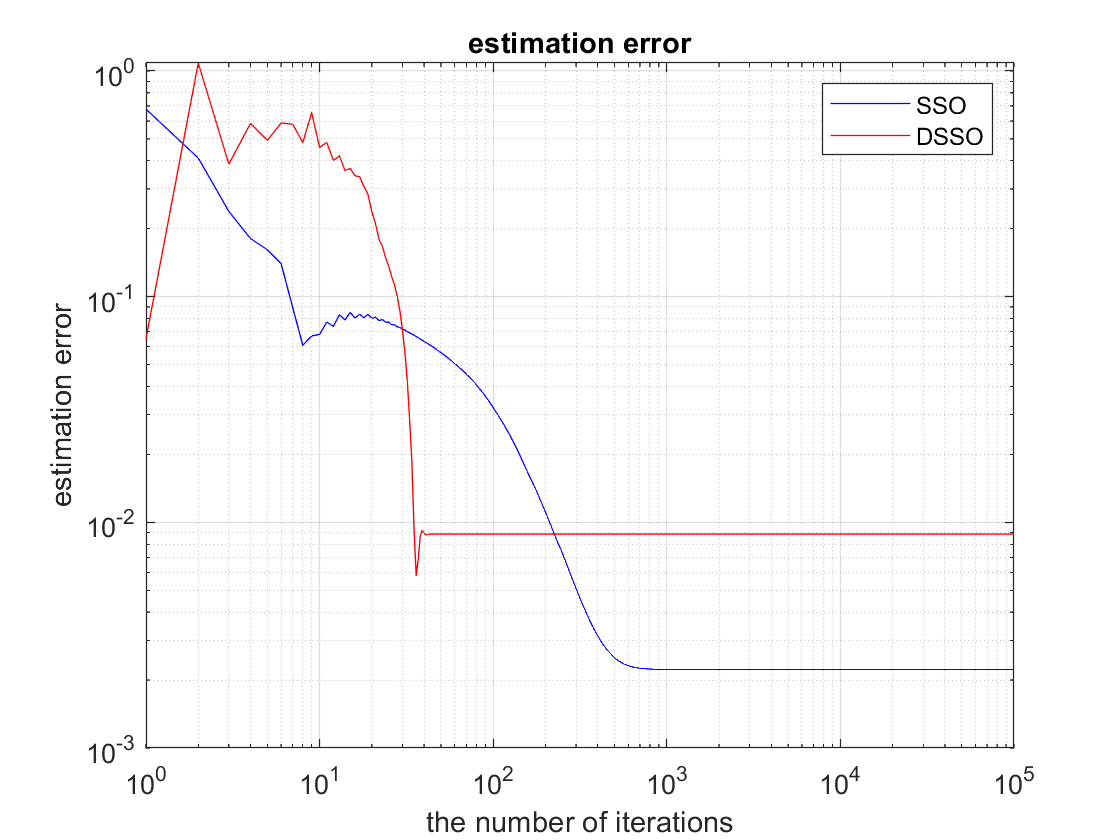
\includegraphics[width=0.75\textwidth]{dynamic_state_error.png} % Adjust width as needed
    \caption{State estimation error of SSO and D-SSO algorithms with suggested values of hyperparameters}
\end{figure}

\begin{figure}[H] % h means "here", can also use t (top), b (bottom), p (page)
    \centering
    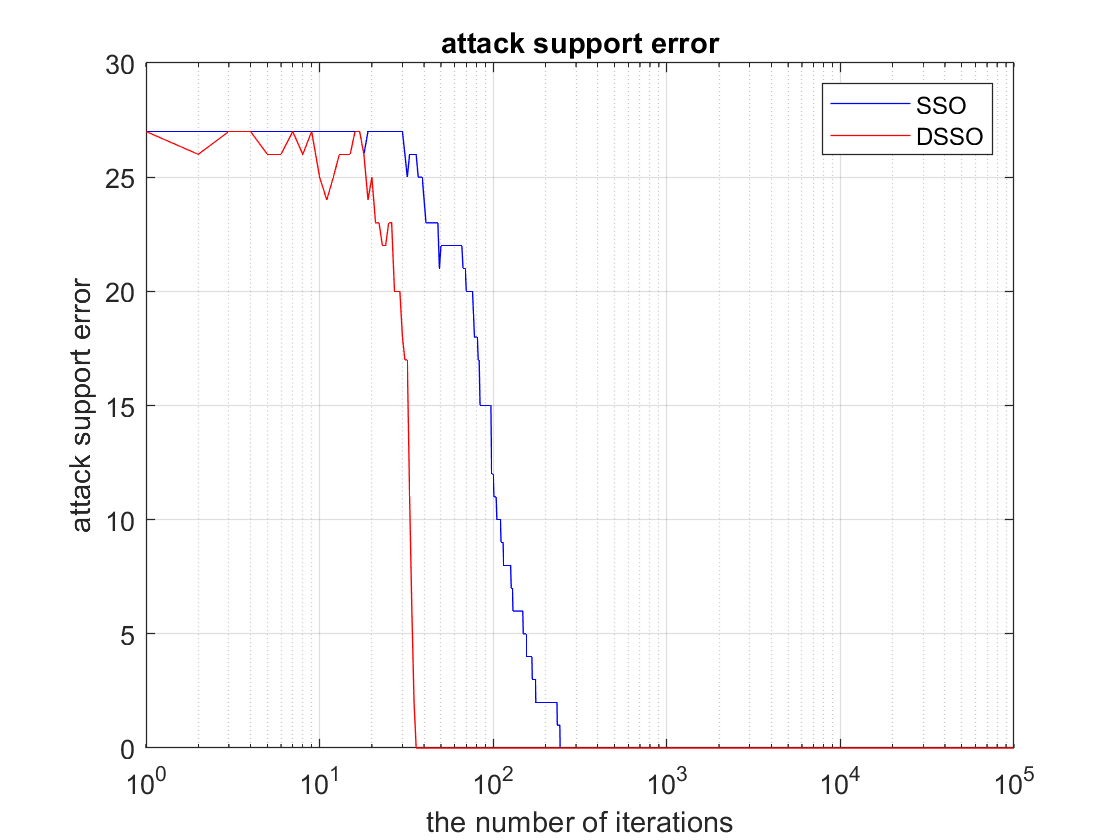
\includegraphics[width=0.75\textwidth]{dynamic_attack_error.png} % Adjust width as needed
    \caption{Attack support error of SSO and D-SSO algorithms with suggested values of hyperparameters}
\end{figure}

Regarding tuning the hyperparameters, it was observed that the following values lead to a way faster results:
For SSO:
\begin{itemize}
	\item $\lambda = 0.1$
	\item $\nu = 0.7$
\end{itemize} 
For D-SSO:
\begin{itemize}
	\item $\lambda = 0.5$
	\item $\nu = 0.9$
\end{itemize} 
Which enjoy a higher value of $\nu$, or a lower inertia, and a higher threshold for soft-thresholding, or a higher value of $\lambda$.

\begin{figure}[H] % h means "here", can also use t (top), b (bottom), p (page)
    \centering
    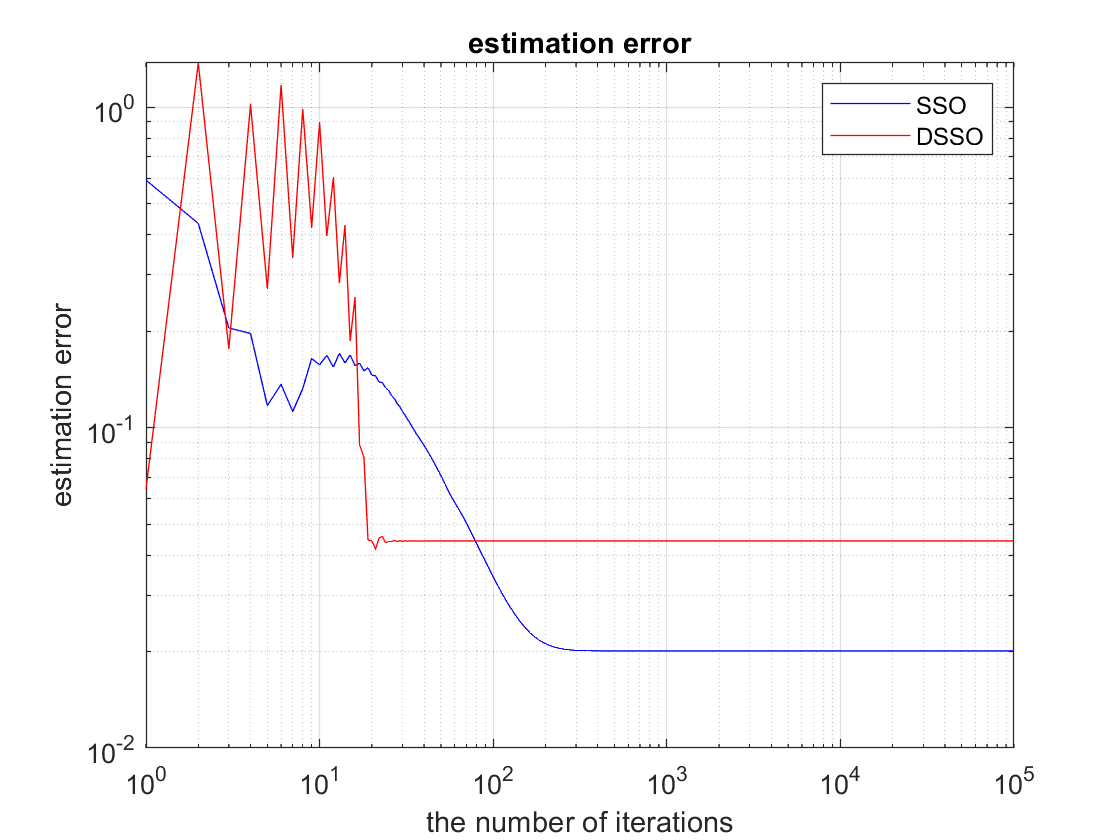
\includegraphics[width=0.75\textwidth]{dynamic_attack_error_modified.png} % Adjust width as needed
    \caption{State estimation error of SSO and D-SSO algorithms with modified values of hyperparameters}
\end{figure}

\begin{figure}[H] % h means "here", can also use t (top), b (bottom), p (page)
    \centering
    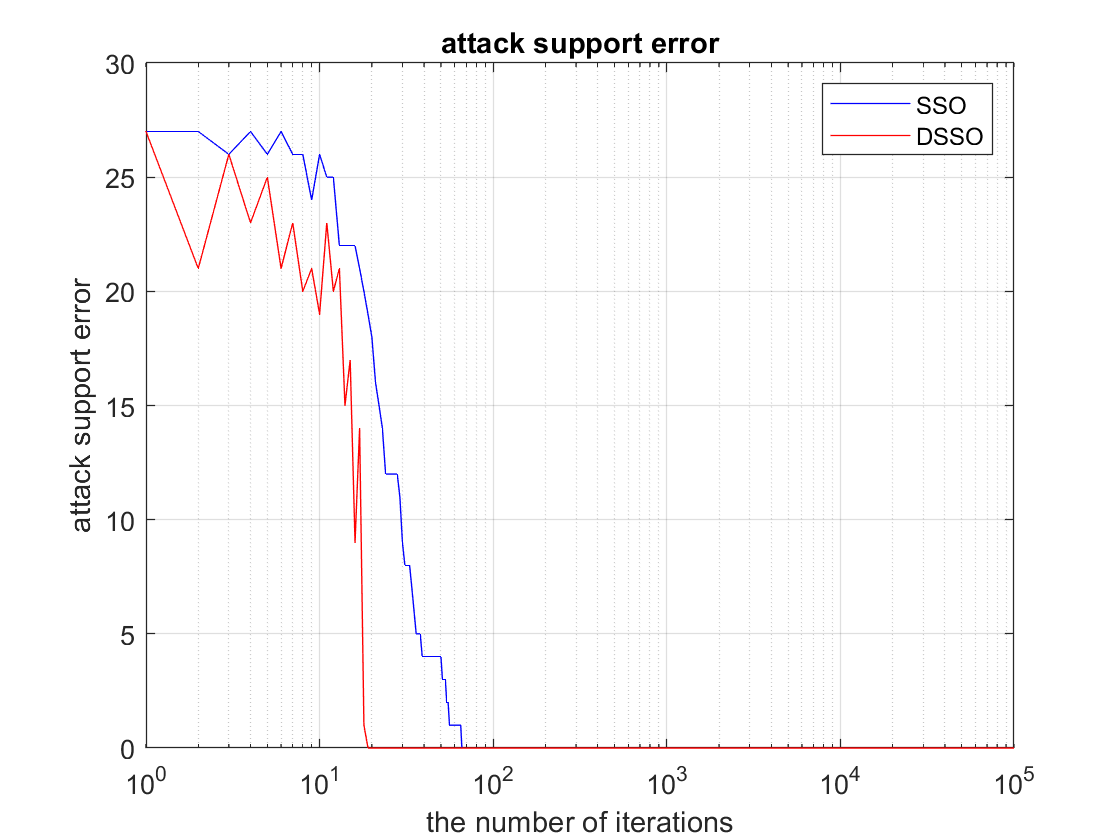
\includegraphics[width=0.75\textwidth]{dynamic_attack_error_modified_2.png} % Adjust width as needed
    \caption{Attack support error of SSO and D-SSO algorithms with modified values of hyperparameters}
\end{figure}

As to enhancing the precision of the estimation, having removed the rows in $C$ corresponding to the attack, an almost zero error was obtained.

\begin{figure}[H] % h means "here", can also use t (top), b (bottom), p (page)
    \centering
    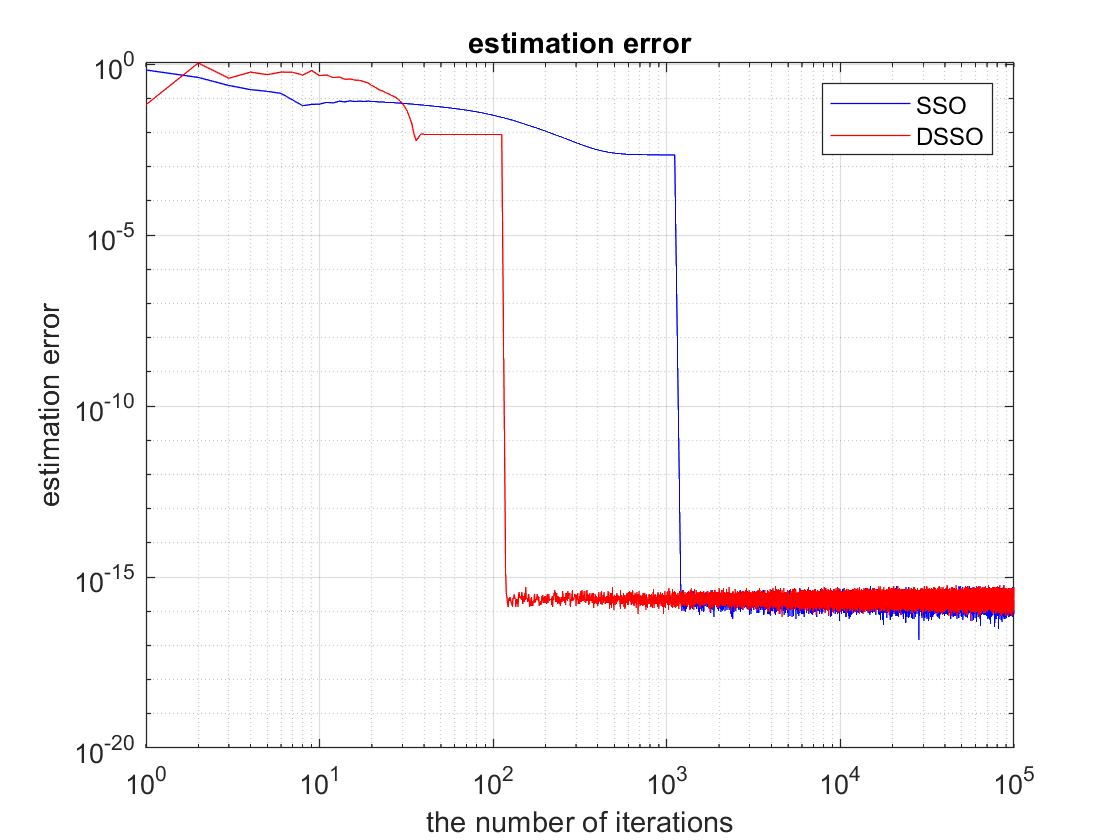
\includegraphics[width=0.75\textwidth]{dynamic_zero_error.png} % Adjust width as needed
    \caption{State estimation error of SSO and D-SSO algorithms with putting aside the sensors under the attack, after correctly estimating the position of the attacks.}
\end{figure}

It can be seen that after convergence, the input of the observer itself introduces high-frequency oscillations. In order to modify this unwanted behavior, the input of the observer is applied only if its inovation is larger than the precision of the sensor; in this case, $10^{-8}$ is considered. The result is going to be as follows:


\begin{figure}[H] % h means "here", can also use t (top), b (bottom), p (page)
    \centering
    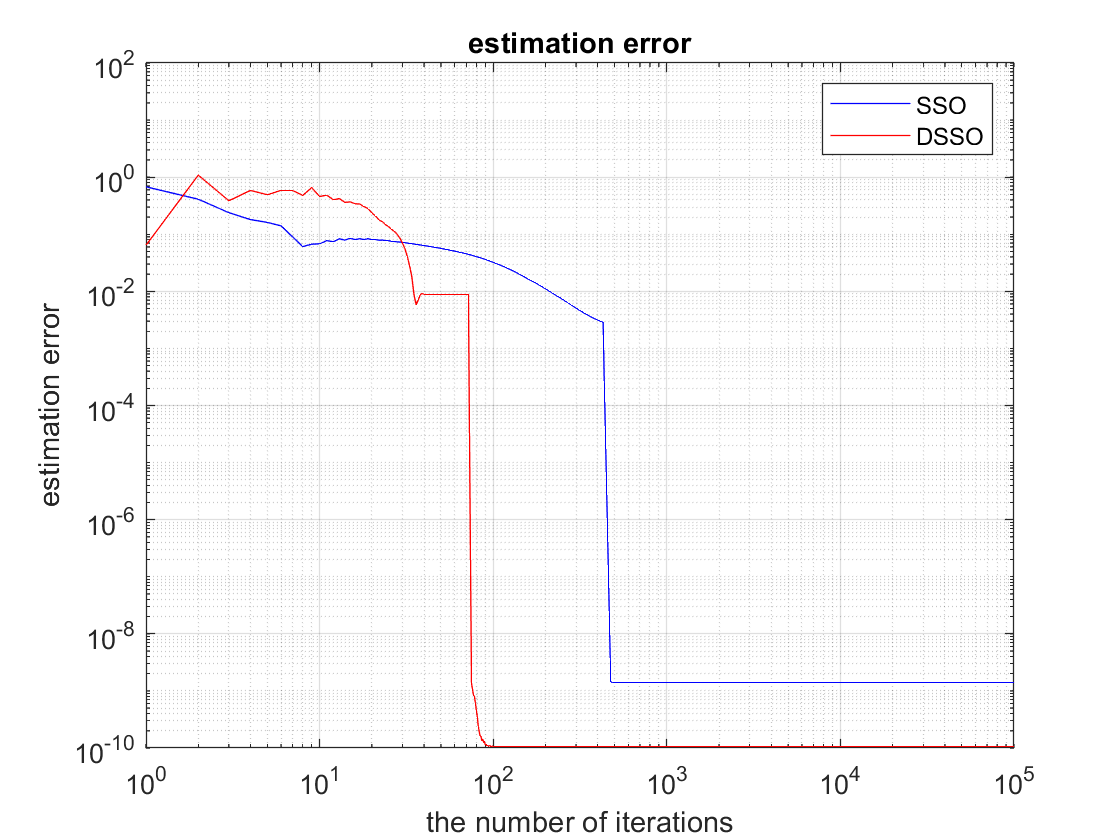
\includegraphics[width=0.75\textwidth]{dynamic_zero_error_clean.png} % Adjust width as needed
    \caption{State estimation error of SSO and D-SSO algorithms with putting aside the sensors under the attack, and cutting the input of the observer when their inovation is smaller than the precision of the sensor.}
\end{figure}
 
\section{conclusion}
It was observed that SSO and D-SSO are capable of secure state estimation of dynamical CPSs under constant values of attacks in finite amount of time. 

Further it was observed that having estimated the position of the attacks, by putting aside the tampered data comming from the attacked sensors, an almost zero estimation error can be obtained. However, in this case, a high-frequency oscillation is introduced due to numerical errors. In order to remove this, the input of the observer is not applied to modify the dynamic of the observer if the difference of the measurements and the system model is smaller than the precision of the sensors.












% !TeX root = ../main.tex
\chapter{Project 04: Target tracking under sparse sensor attacks}

\section{Objectives}
The aim of this project is to track the position of a device using RSS fingerprinting setting. In this project, we are given the dictionary $D$, and it is requested to track the position of the device having a given noisy and attack corrupted measurements.

\section{Setting of the problem}
In this task, the room is gridded into 36 cells and 20 sensors are used in the training phase. In addition, it is assumed that during the training step has done in an offline manner, and therefore, the dictionary $D$ is assumed to be attack free. During the ``application'' phase, which it is required to track the position a device, 4 sensors are under the attack, and the task is to track the position of a target, or targets in this room given the dynamical evolution of the system, and also find which sensors are under attack. The model has the following dynamics:

\begin{equation}
\begin{cases}
x(k+1) = A\,x(k) \\
y(k) = D\,x(k) + \tilde{a} + \eta
\end{cases}
\end{equation}

where the measurement vector $y(k)$ is corrupted by a constant attack vector $\tilde{a}$ and noise $\eta$.

The same as the previous project, the problem to be solved is sparse. The same as \textit{task 2}, a full weighted Lasso needs to be considered, since the position of a target or some targets in a room are assumed to be sparse:

\begin{equation}
\min_{x \in \mathbb{R}^{n}, a \in \mathbb{R}^{q}} \left\| G \begin{pmatrix} x \\ a \end{pmatrix} - y \right\|_2^2 + \lambda_1 \| x \|_1 + \lambda_2 \| a \|_1
\end{equation}
where,
\[
G = (D, I)
\]

Here, in order not to face numerical problems, G should be normalized, this is done using \texttt{normalize( )} command in MATLAB. In this way, we make sure that $G$ and $I$ are of the same scale.

\section{Implementation of the algorithm}
\subsection{Luenberg Observer}
Since the attacks is assumed to be constant, when shaping the observability matrix, at least 2 columns are going to be linearly dependent, and hence, some states are going to be unobservable. Therefore, a Luenberg observer cannot be adopted. However, Sparse observers still can be used in order to accomplish the task.

\subsection{SSO for tracking}
SSO can be adopted in order to solve the problem; however, the terms regarding the state needs to be sparsified

\textbf{Initialization:} \(\tau > 0\), \(\hat{x}(0) \in \mathbb{R}^{n}\), \(\hat{a}(0) \in \mathbb{R}^{q}\), e.g., \(\hat{x}(0) = 0\), \(\hat{a}(0) = 0\)

\textbf{For} \( k = 0, \dots, T_{\max} \),

\begin{align}
    y(k) &= D_1x(k) + a\\
    \hat{y}(k) &= D_1\hat{x}(k) + \hat{a}\\
    \hat{x}(k+1) &= S_{\nu_1\lambda_1} [A\hat{x}(k) - \nu A D_1^\top (\hat{y}(k) - y(k))] \\
    \hat{a}(k+1) &= S_{\nu_2\lambda_2} [\hat{a}(k) - \nu I_1^\top (\hat{y}(k) - y(k))] \\
    x(k+1) &= A x(k)
\end{align}
where $D_1$ and $I_1$ are normalized $D$ and $I$

The suggested values of hyperparameters used in this algorithm are:
\begin{itemize}
	\item $\lambda_1 = \lambda_2 = 10$
	\item $\nu_1 = \frac{0.99}{\|D_1\|_2^2}$
	\item $\nu_2 = \frac{0.99}{\|I_1\|_2^2}$
\end{itemize} 
To enhance the convergence rate the following values were used for SSO:
\begin{itemize}
	\item $\lambda_1 = \lambda_2 = 10$
	\item $\nu_1 = \frac{2*0.99}{\|D_1\|_2^2}$
	\item $\nu_2 = \frac{2*0.99}{\|I_1\|_2^2}$
\end{itemize} 
To check the perforamance, the performance needs to be cleaned. In the sense that since the value of the state can be either 0 or 1,  a threshold should be considered so that for the values of the states lower than that threshold the state becomes 0 and otherwise, 1. A threshold of 0.1 was considered for this algorithm.
\subsection{D-SSO for tracking}
The taylored D-SSO for tracking is as follows:

\textbf{For} \( k = 0, \dots, T_{\max} \),

\begin{align}
    y(k) &= Cx(k) + a(k) \\
    \hat{y}(k) &= C\hat{x}(k) + \hat{a}(k) \\
    \hat{x}(k+1) &= S_{\nu\lambda}[A\hat{x}(k) - L (\hat{y}(k) - y(k))] \\
    \hat{a}(k+1) &= S_{\nu\lambda} [\hat{a}(k) - \nu (\hat{y}(k) - y(k))] \\
    x(k+1) &= A x(k)
\end{align}

Where $L$ is designed such that, $eig(A - LC) = 0$. In order not to face numerical issues, \texttt{place()} command is used by randomized desirable eigenvalues close enough to zero, with standard deviation of 0.01. The value of hyperparameters used in this algorithm are:
\begin{itemize}
	\item $\lambda = 0.01$
	\item $\nu = 0.05$
\end{itemize} 

The cleaning threshold used for the states is 0.6.

\section{Results}
\subsection{State Support Error}
It is observed that both SSO and DSSO after some iterations can correctly track the position of the target. In terms of performance, SSO correctly tracks the position of the target after 25 iterations with enhanced parameters and after 32 iterations for the suggested hyperparameters. On the otherhand, it took 185 iteration for DSSO to perfectly track the target, which is considerably slower.

\begin{figure}[H]
    \centering
    \subfloat[State support error of SSO using suggested hyperparameters]{
        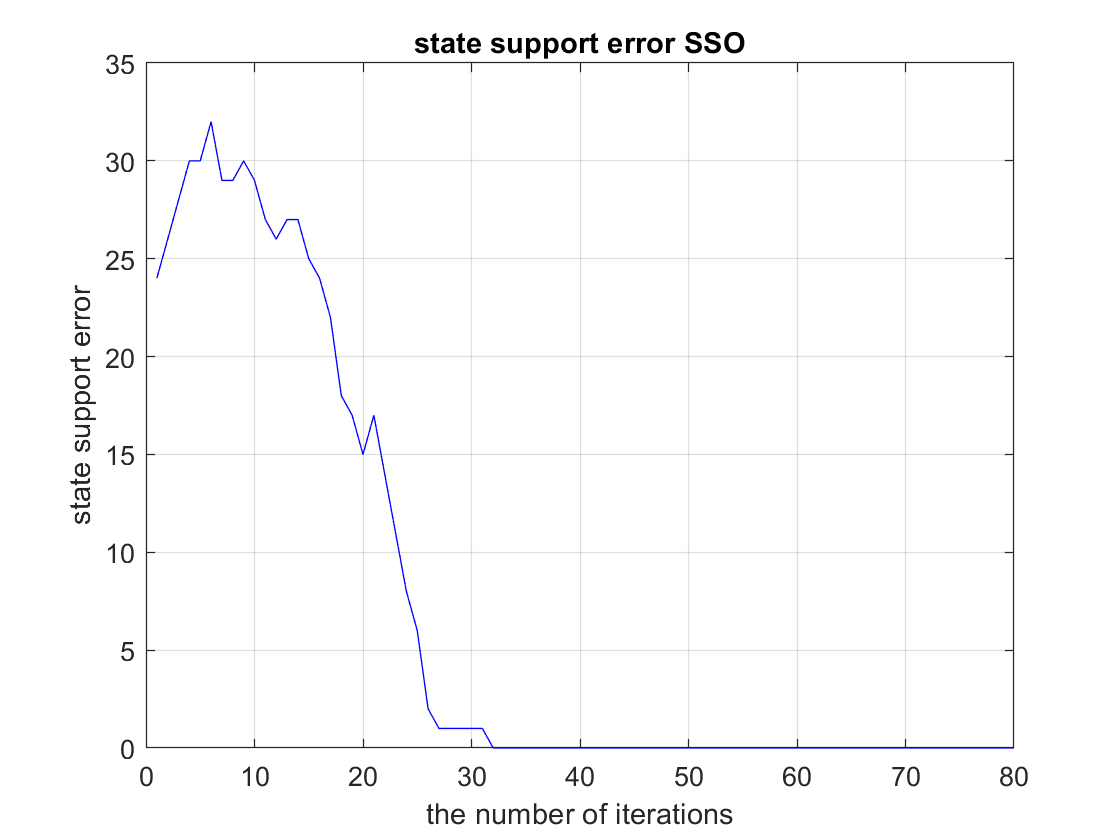
\includegraphics[width=0.45\textwidth]{state_support_error_SSO_suggested.png} % Adjust width as needed
    }
    \hspace{1cm} % Adjust the space between the two figures
    \subfloat[State support error of SSO using enhanced hyperparameters.]{
        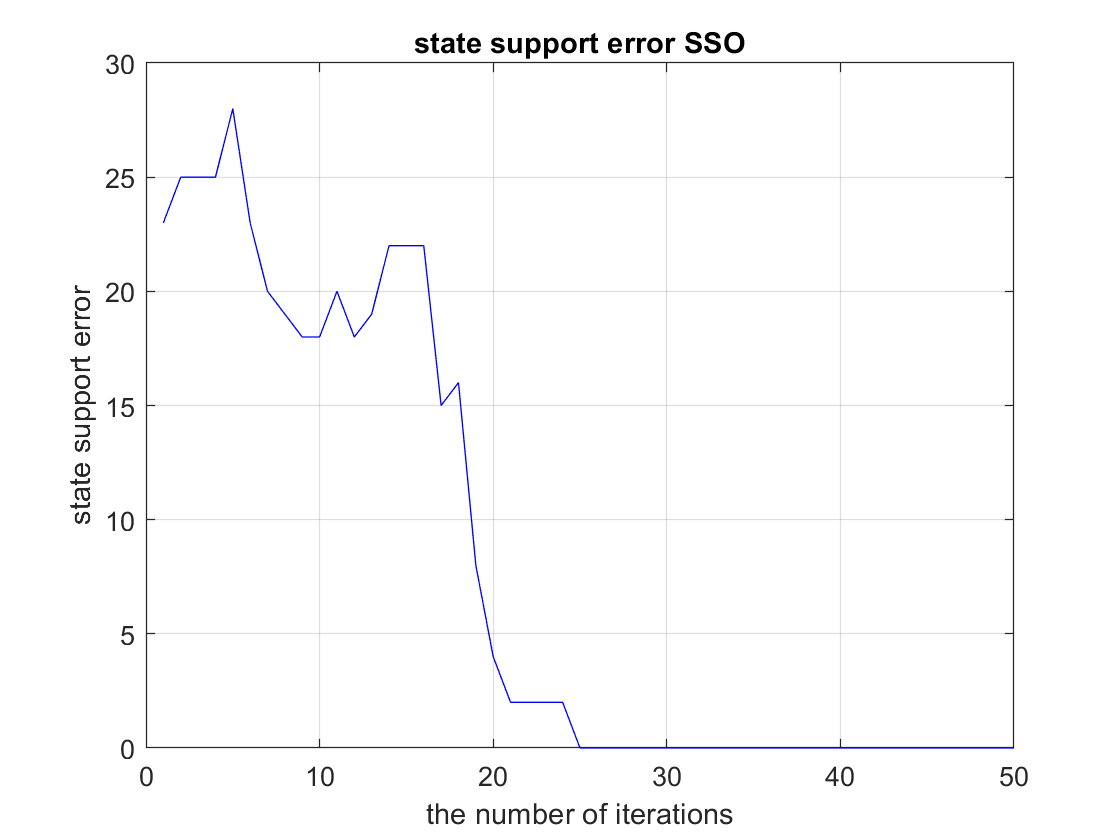
\includegraphics[width=0.45\textwidth]{state_support_error_SSO.png} % Adjust width as needed
    }
    \caption{Comparison of the convergence rate of state support error of SSO using suggested and enhanced hyperparameters for running the algorithm}
\end{figure}

\begin{figure}[H]
    \centering
    \subfloat[tracking performance using suggested hyperparameters]{
        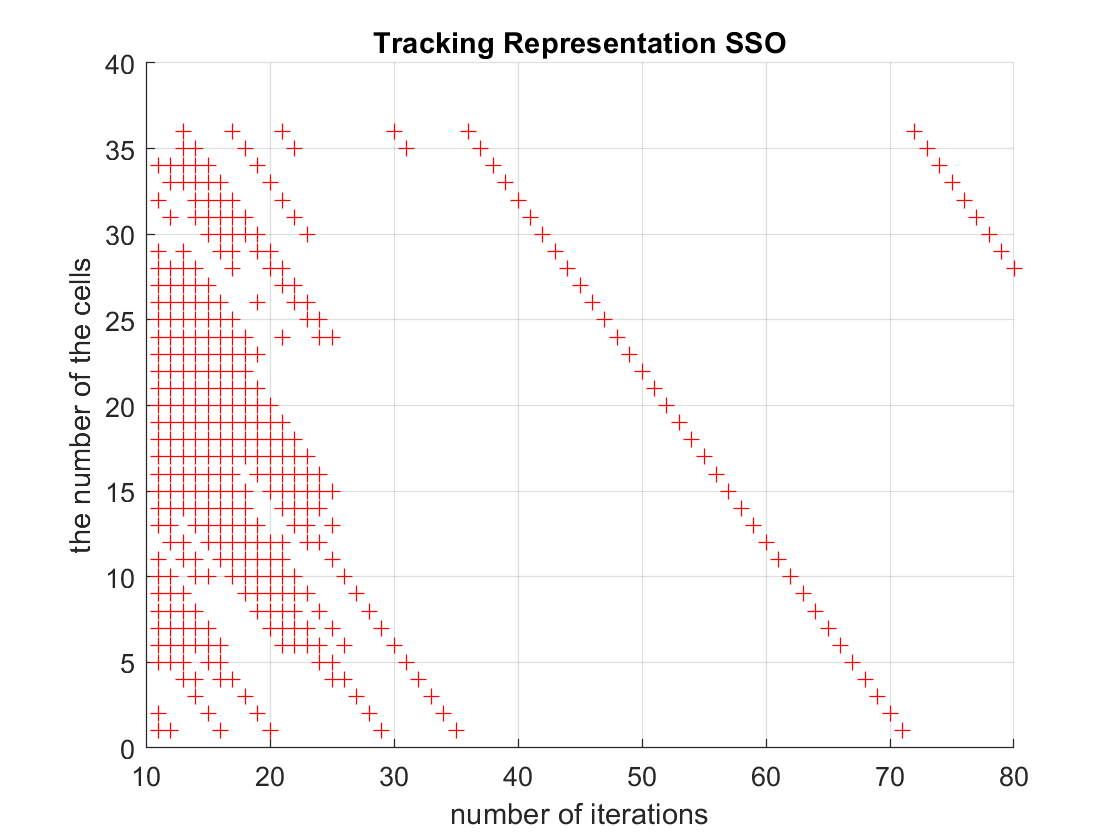
\includegraphics[width=0.45\textwidth]{tracking_SSO_suggested.png} % Adjust width as needed
    }
    \hspace{1cm} % Adjust the space between the two figures
    \subfloat[tracking performance using enhanced hyperparameters.]{
        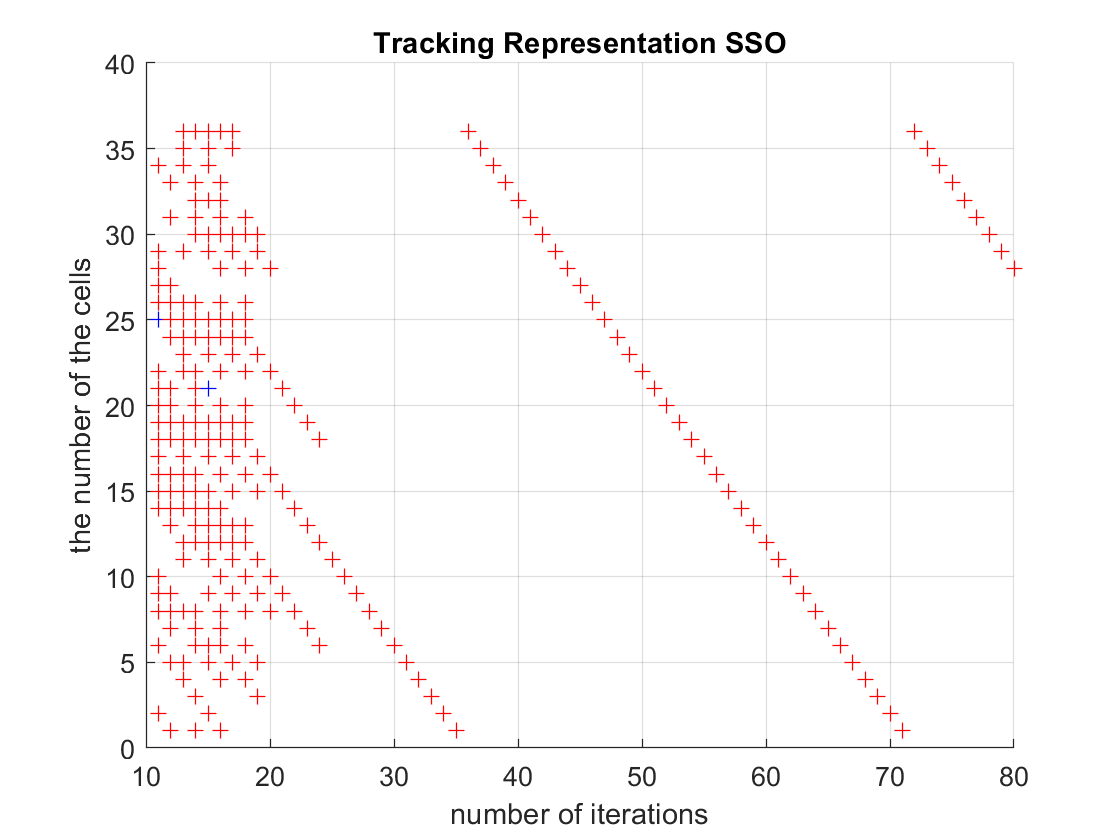
\includegraphics[width=0.45\textwidth]{tracking_SSO.png} % Adjust width as needed
    }
    \caption{Comparison of tracking performance of SSO using suggested and enhanced hyperparameters for running the algorithm}
\end{figure}

As it was also mentioned in the second project, the DSSO, which is the dynamic counterpart of IJAM, does not have a smooth transient, which in turn introduces problem when soft-thresholding is applied. Here, the parameters were turned so that it can solve the problem. However, again a two step approach as it is discussed in the further discussion of the second project can be adopted. Here, a normal approach was adopted and a slower performance from DSSO was observed, which can be since in the following plots.

\begin{figure}[H] % h means "here", can also use t (top), b (bottom), p (page)
    \centering
    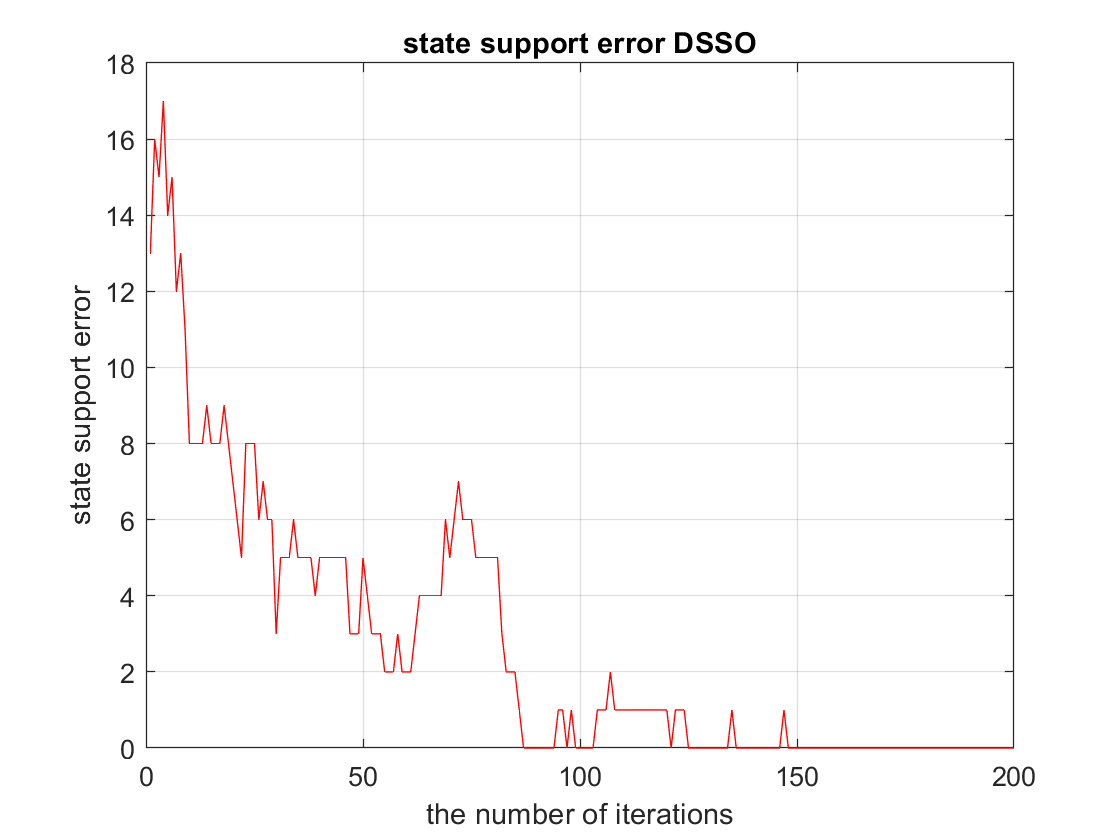
\includegraphics[width=0.75\textwidth]{state_support_error_DSSO.png} % Adjust width as needed
    \caption{State support error of DSSO; it can be seen that it is considerably slower than SSO.}
\end{figure}

\begin{figure}[H] % h means "here", can also use t (top), b (bottom), p (page)
    \centering
    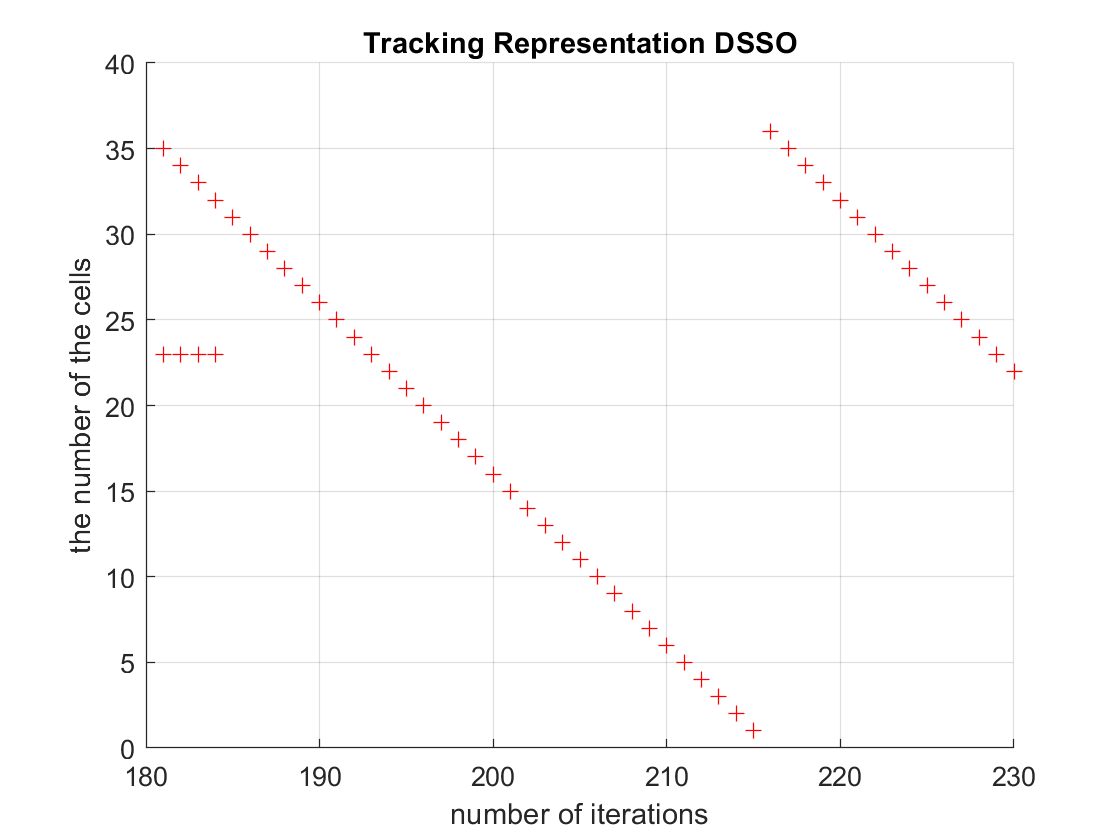
\includegraphics[width=0.75\textwidth]{tracking_DSSO.png} % Adjust width as needed
    \caption{Tracking performance of DSSO}
\end{figure}
\subsection{Attack Support Error:}
Regarding this performance metric, it need to be mentioned that the implemented DSSO is unable to estimate the position of the attacks correcty, and the number of attack support error remain constant on 11. On the other hand, attack support error in the case of SSO convergese to 0 after 20 iterations.
\begin{figure}[H] % h means "here", can also use t (top), b (bottom), p (page)
    \centering
    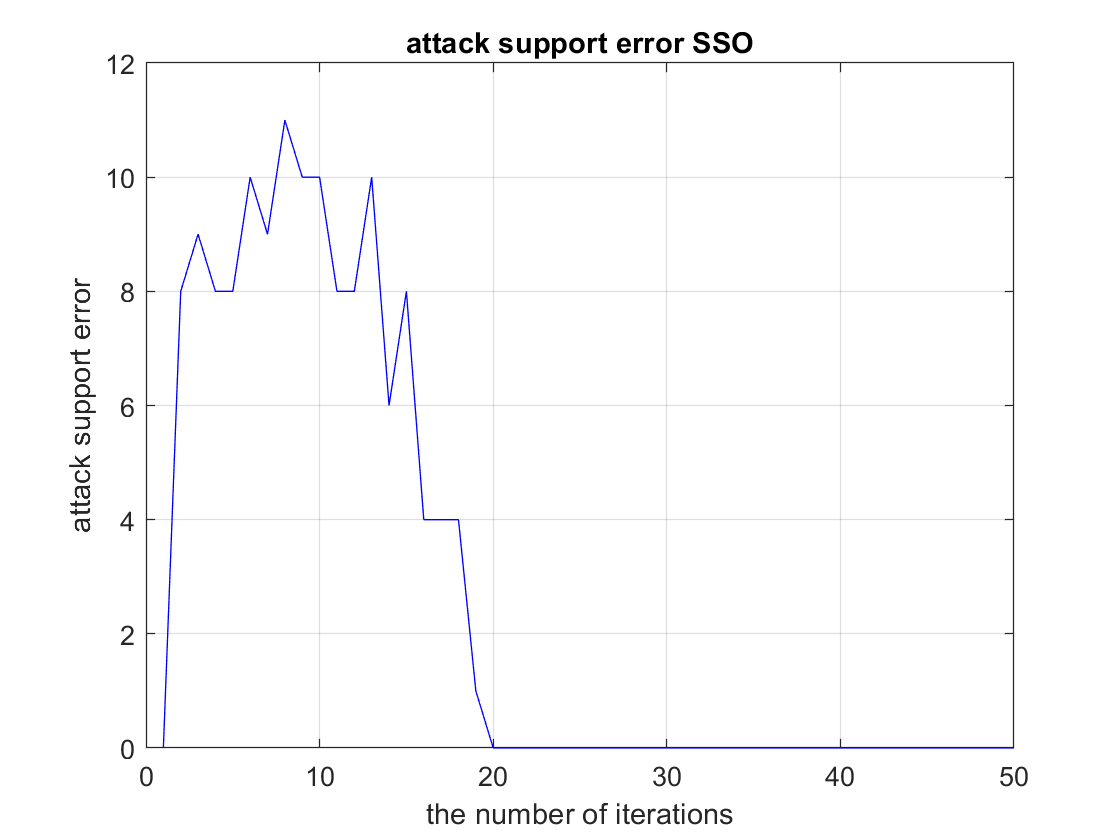
\includegraphics[width=0.75\textwidth]{attack_support_error_SSO.png} % Adjust width as needed
    \caption{Attack support error of SSO}
\end{figure}

\begin{figure}[H] % h means "here", can also use t (top), b (bottom), p (page)
    \centering
    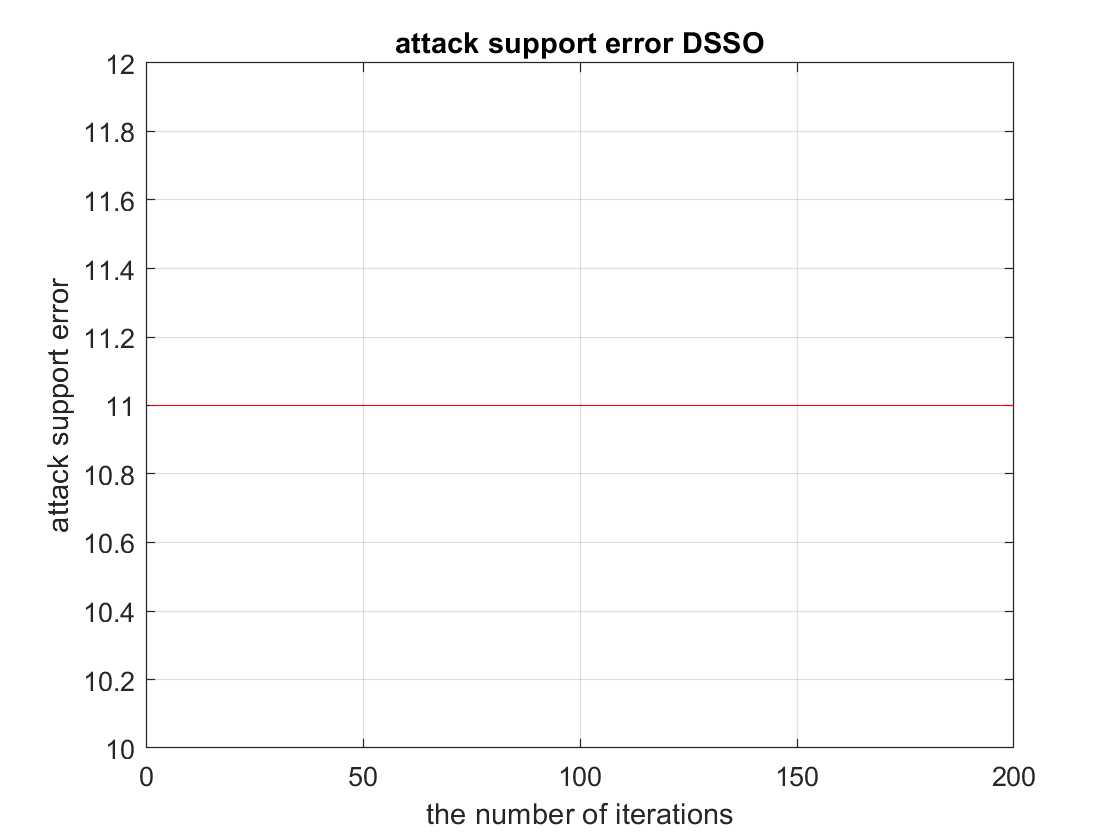
\includegraphics[width=0.75\textwidth]{attack_support_error_DSSO.png} % Adjust width as needed
    \caption{Attack support error of DSSO; the attack support error does not improves over time; since the threshold for cleaning was relatively large, no cleaning threshold was adopted here.}
\end{figure}


\section{Conclusion}
In conclusion, for performing a fingerprint tracking with constant attack, Luenberg observer cannot be used, since the extended observability matrix does not become full rank. Nonetheless, using SSO and DSSO taylored for this problem, which requires introducing soft-thresholding also for the states, tracking was achieved. 

SSO showed a noticably faster performance in tracking compared to DSSO, and unlike DSSO, SSO was able to detect correctly the position of the attacks, DSSO. SSO has a smooth transient and when soft-thresholding is introduced to the problem, it can solve the problem. In the case of DSSO, the introduction of soft-thresholding disrupt the performance of DSSO, owing to the fact that DSSO have an oscillatory transient behavior.

A proposal is that implement DSSO in two steps to enhance its behavior:
\begin{enumerate}
	\item Running the algorithm so that the transient phase pases without applying soft-thresholding.
	\item Applying soft-thresholding to the state, now that the transient is passed.
\end{enumerate}

Doing so, a better result from DSSO may be obtained.










% !TeX root = ../main.tex
\chapter{Project 05: Distributed Target localization under sparse sensor attacks}

\section{Objectives}
The aim of this project is to localize the position of a device using RSS fingerprinting setting. However, unlike the second project, this time the aim is to do the task using distributed consensus-based optimization by nodes. In this project, we are given the dictionary $D$, and it is requested to localize the position of the device having a given measurement which is corrupted by attacks.

\section{Setting of the problem}
The localization problem is set in 10 by 10 squaremeters room. The room is gridded into 100 cells and 20 sensors are used in the training phase. In addition, it is assumed that during the training step has done in an offline manner, and therefore, the dictionary $D$ is assumed to be attack free. The difference in this setting is that each node knows its own row in the matrix $D$ and the matrix $D$ is not known globally, due to privacy matters. It is assumed that the sensors enjoy computational power and therefore they update their own state and share it with their neighbors. Further, a matrix $Q$ is given, determining the topology of the network, or the weights by which the nodes perform the average of theshared states of their neighbors. The communication link are assumed to be secure and only the sensors are under the attack. The number of attacked sensors the same as the project 2 is 5.
\begin{figure}[H] % h means "here", can also use t (top), b (bottom), p (page)
    \centering
    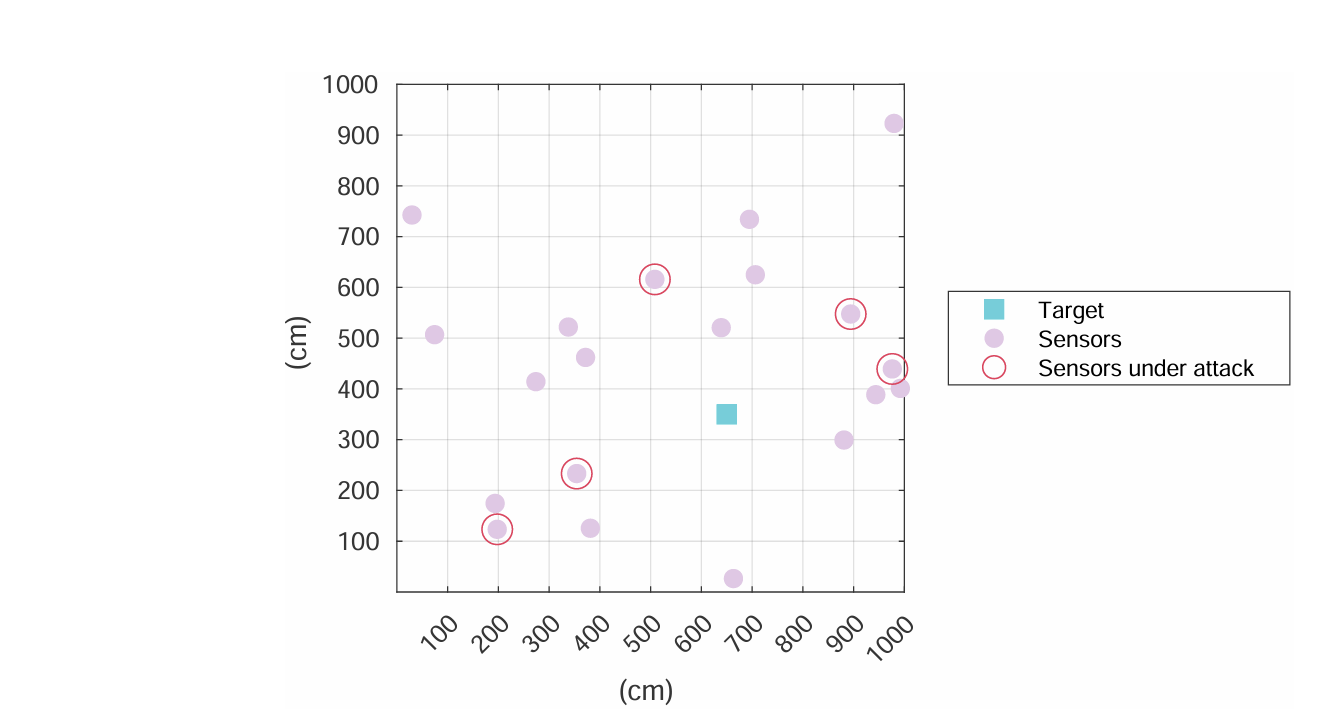
\includegraphics[width=0.75\textwidth]{localization_setting.png} % Adjust width as needed
    \caption{The graphical setting of the problem; reported from the project 2025 file.}
\end{figure}
The dimensions of the problem are as follows:
\begin{itemize}
	\item the number of the cells (states) $n = 100$,  states can be 0 or 1, and only 1 state can be 1.
	\item the number of the sensors, or nodes, length of the measurement sensor $q = 20$, 
	\item the number of the attacks $h = 5$
\end{itemize}

It is required to solve the problem considering two network topology: star and ring. The relaxed problem to be solved in order to solve the distributed consensus-based optimization problem is going to be as follows:

\begin{equation}
\min_{\{x^{(i)}, a^{(i)}\}_{i=1}^q} 
\sum_{i=1}^q \left\| C x^{(i)} + a^{(i)} - y^{(i)} \right\|_2^2
+ \lambda_1 \sum_{i=1}^q \left\| x^{(i)} \right\|_1
+ \lambda_2 \sum_{i=1}^q \left\| a^{(i)} \right\|_1
+ \frac{\lambda}{2} \sum_{i,j \in \mathcal{N}(i)} \left\| x^{(i)} - x^{(j)} \right\|_2^2
\end{equation}


\section{Implementation of the algorithm}
\subsection{DISTA for Ring Topology}
The topology of the network in the ring problem is as follows:
\begin{figure}[H] % h means "here", can also use t (top), b (bottom), p (page)
    \centering
    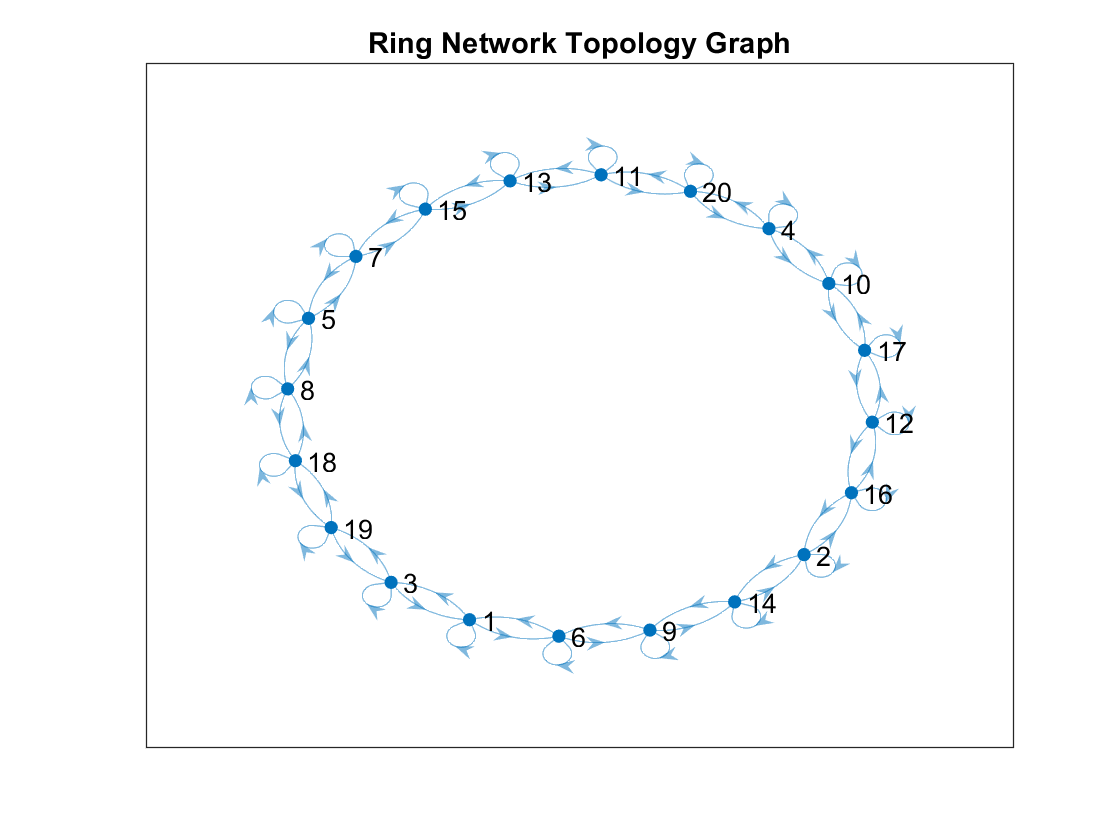
\includegraphics[width=0.75\textwidth]{ring-topology.png} % Adjust width as needed
    \caption{The graph of the communication link in Ring topology.}
\end{figure}
In this topology each node has the same number of data with which they communicate. 

The iterative algorithm to use for solving the problem is DISTA, with the difference that since the state is also sparse, it is needed to apply soft-thresholding to both the states and the attack.

\begin{equation}
\begin{pmatrix}
x^{(i)}(k+1) \\
a^{(i)}(k+1)
\end{pmatrix}
=
\mathcal{S}_{\nu \lambda} \left[
\sum_{j=1}^{q} Q_{i,j}
\begin{pmatrix}
x^{(j)}(k) \\
a^{(j)}(k)
\end{pmatrix}
-
\nu G^{(i)\top} \left( y^{(i)} -
G^{(i)}
\begin{pmatrix}
x^{(i)}(k) \\
a^{(i)}(k)
\end{pmatrix}
\right)
\right]
\end{equation}


The suggested parameters for this problem is:
\begin{itemize}
	\item $\lambda = 1$
	\item $\nu = 0.01*\|G\|_2^{-2}$
\end{itemize}

This algorithm is run until the difference of the two consequitive states becomes lower that $\delta = 10^{-8}$.

Once this goal is achieved, the state position needs to be cleaned. That is, 0 should be allocated to the states with values smaller than a certain threshold, and 1 should be allocated otherwise. Since we know that we have one target to track, we can simply allocate 1 to the maximum of the state for each node. Regarding the attacks, a threshold of 0.05 is used in the Ring topology. It is,further, expected that at the end of the simulation, a consensus is reached in the network, thereby all the nodes have the same estimation of the position of the target, as well as the position of the attacked sensors.

\subsection{DISTA for Star Topology}
The topology of the network in the star problem is as follows:
\begin{figure}[H] % h means "here", can also use t (top), b (bottom), p (page)
    \centering
    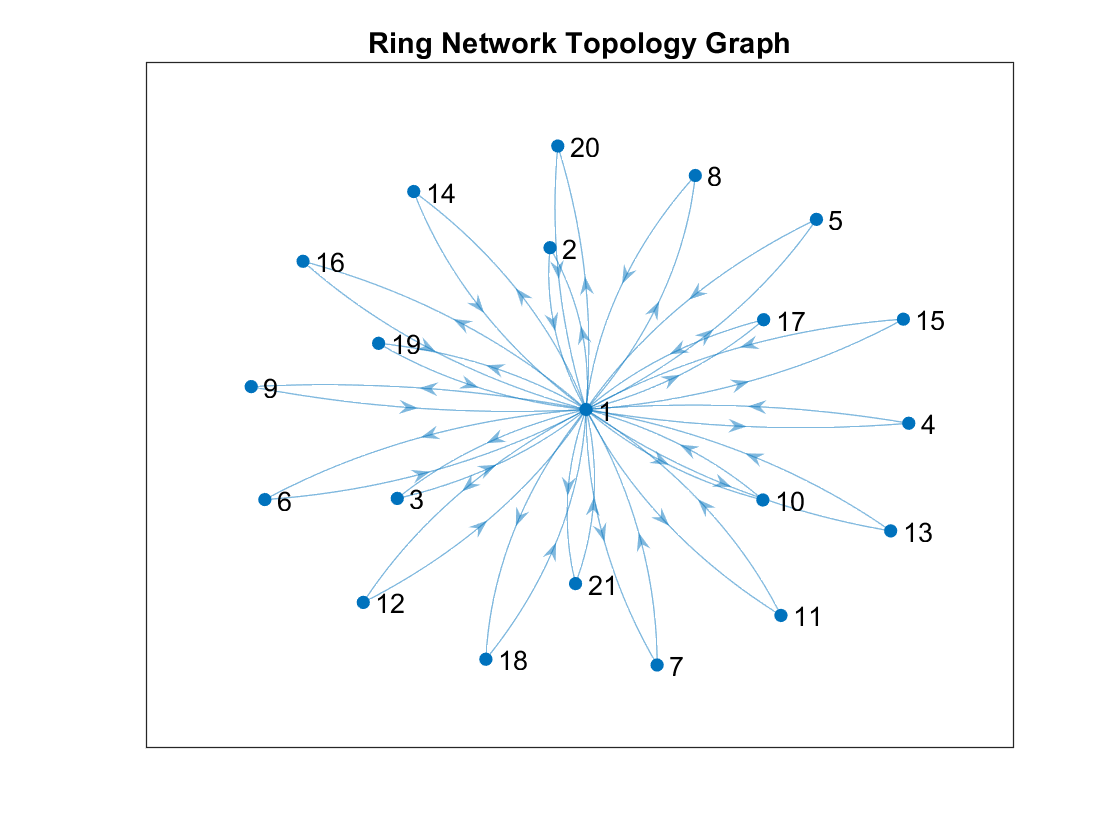
\includegraphics[width=0.75\textwidth]{star-topology.png} % Adjust width as needed
    \caption{The graph of the communication link in Star topology; the node zero at each iteration computes the average state of all the nodes and transmit it to all the nodes to perform their calculations.}
\end{figure}
In this configuration, there is one super node, node 0, where it receives the state of all the nodes, calculate the mean, and send the calculated average of the states to the nodes. Afterwards, each node perform distributed gradient descent modifying the average state received from the super node.

The same algorithm of the Ring topology is used here. However, before updating the states, the mean is calculated by the super node, and then the nodes perform the calculations.
\begin{equation}
\begin{pmatrix}
x^{0}(k) \\
a^{0}(k)
\end{pmatrix} = \sum_{j=1}^{q} Q_{1,j}^{j} \begin{pmatrix}
x^{j}(k) \\
a^{j}(k)
\end{pmatrix}
\end{equation}

\begin{equation}
\begin{pmatrix}
x^{(i)}(k+1) \\
a^{(i)}(k+1)
\end{pmatrix}
=
\mathcal{S}_{\nu \lambda} \left(
\sum_{j=1}^{q} Q_{i,j}
\begin{pmatrix}
x^{(j)}(k) \\
a^{(j)}(k)
\end{pmatrix}
-
\nu G^{(i)\top} \left( y^{(i)} -
G^{(i)}
\begin{pmatrix}
x^{(i)}(k) \\
a^{(i)}(k)
\end{pmatrix}
\right)
\right)
\end{equation}

The suggested parameters for this problem is:
\begin{itemize}
	\item $\lambda = 1$
	\item $\nu = 0.01*\|G\|_2^{-2}$
\end{itemize}

This algorithm is run until the difference of the two consequitive states becomes lower that $\delta = 10^{-8}$.

The same as the Ring topology, after the algorithm stops, we need to clean the data. The cleaning threshold for the attack is 0.07 for the star topology.

In an attemp to enhance the performance of the algorithm the following values were used as hyperparameters:
\begin{itemize}
	\item $\nu = 0.012*\|G\|_2^{-2}$
	\item $\lambda= 1.3$
\end{itemize}


\section{Results}
It was observed that both Ring and Star topology reached the consensus after a finite number of iterations. Furthermore, all the nodes correctly estimated the position of the target and the attacked nodes. In the following plots suggesting this result is represented. 
\begin{figure}[H]
    \centering
    \subfloat[The head map of the state support vector of different nodes after the consensus in the Ring topology.]{
        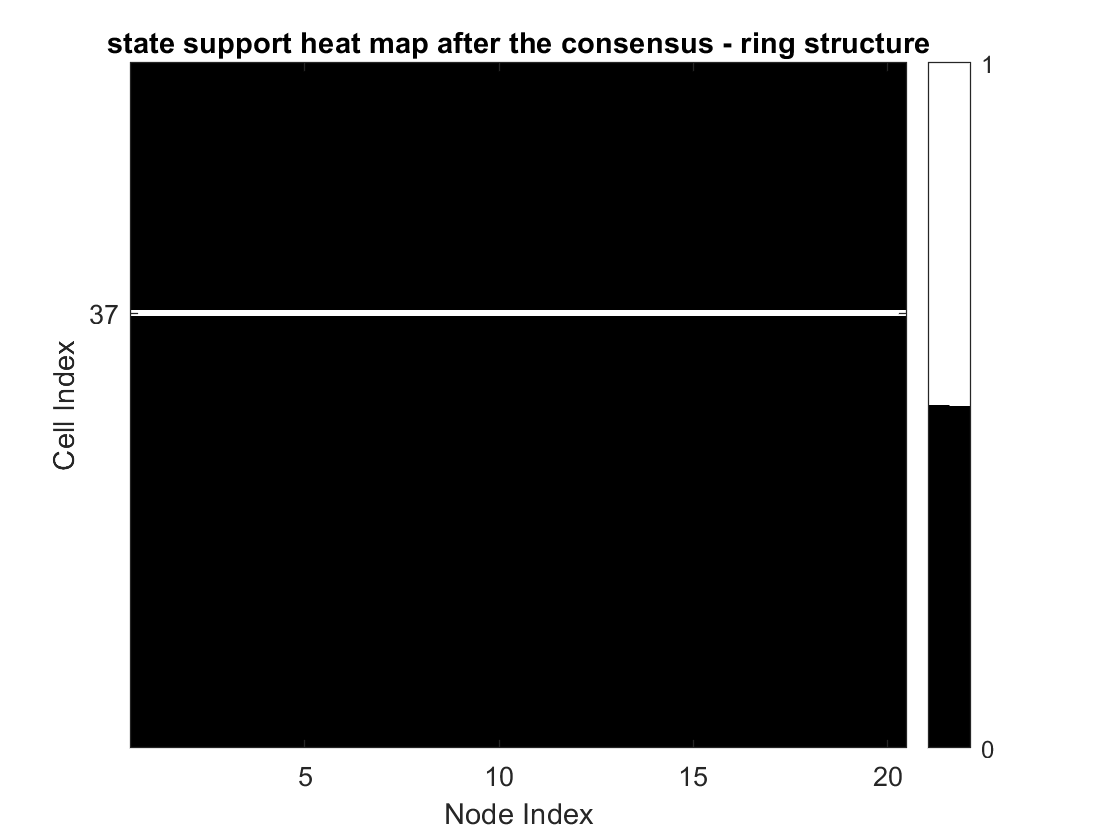
\includegraphics[width=0.45\textwidth]{state-ring.png} % Adjust width as needed
    }
    \hspace{1cm} % Adjust the space between the two figures
    \subfloat[The head map of the attack support vector of different nodes after the consensus in the Ring topology.]{
        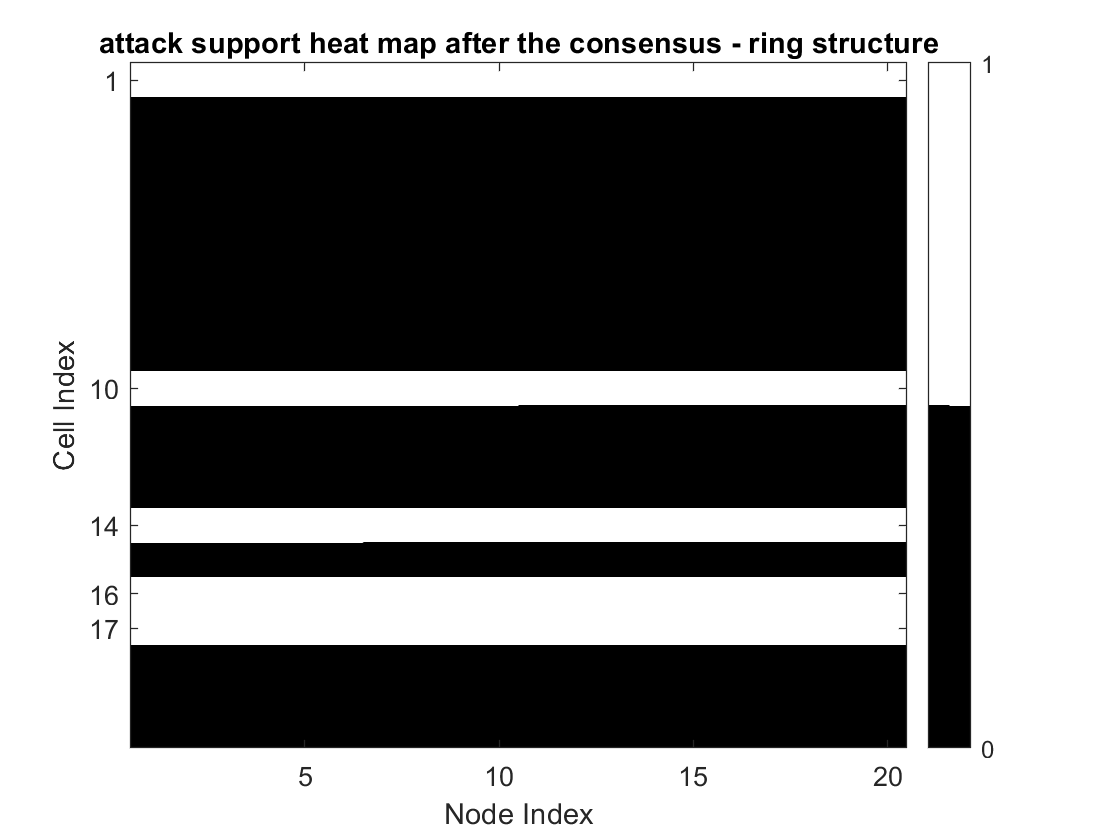
\includegraphics[width=0.45\textwidth]{attack-ring.png} % Adjust width as needed
    }
    \caption{Comparison of state and attack support vectors after consensus in the Ring topology.}
\end{figure}

\begin{figure}[H]
    \centering
    \subfloat[The head map of the state support vector of different nodes after the consensus in the Star topology.]{
        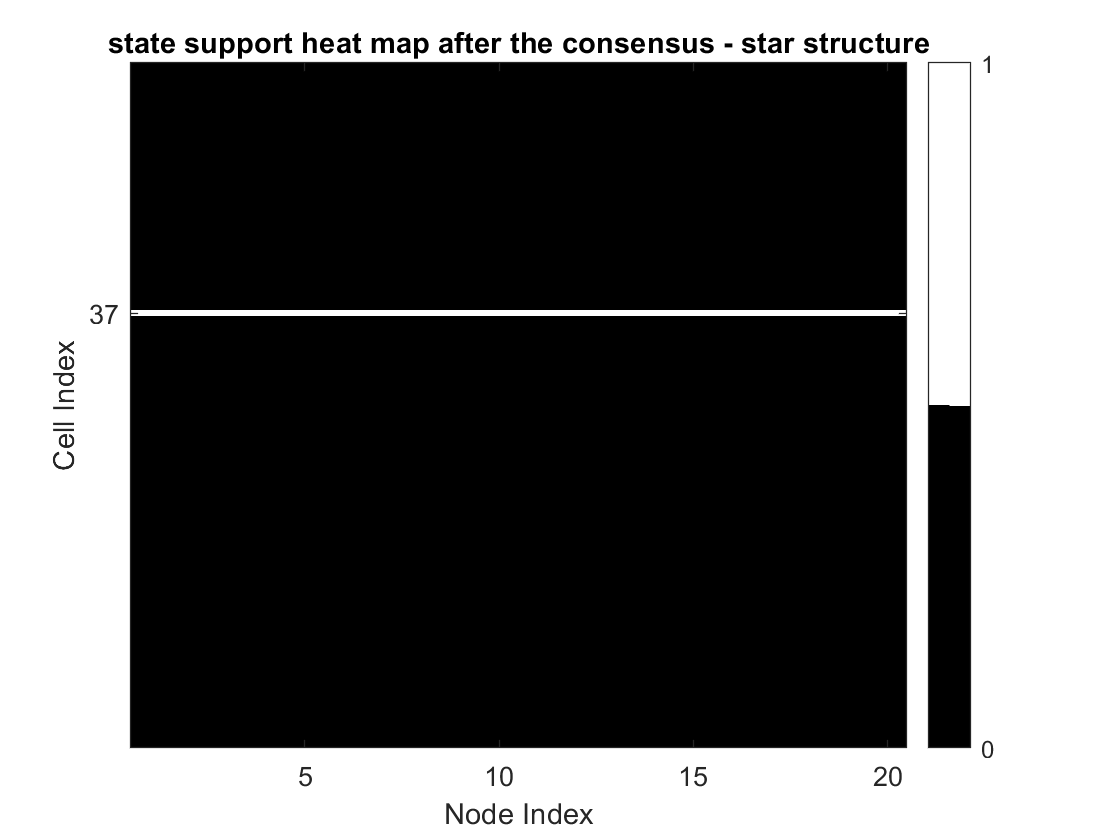
\includegraphics[width=0.45\textwidth]{state-star.png} % Adjust width as needed
    }
    \hspace{1cm} % Adjust the space between the two figures
    \subfloat[The head map of the attack support vector of different nodes after the consensus in the Star topology.]{
        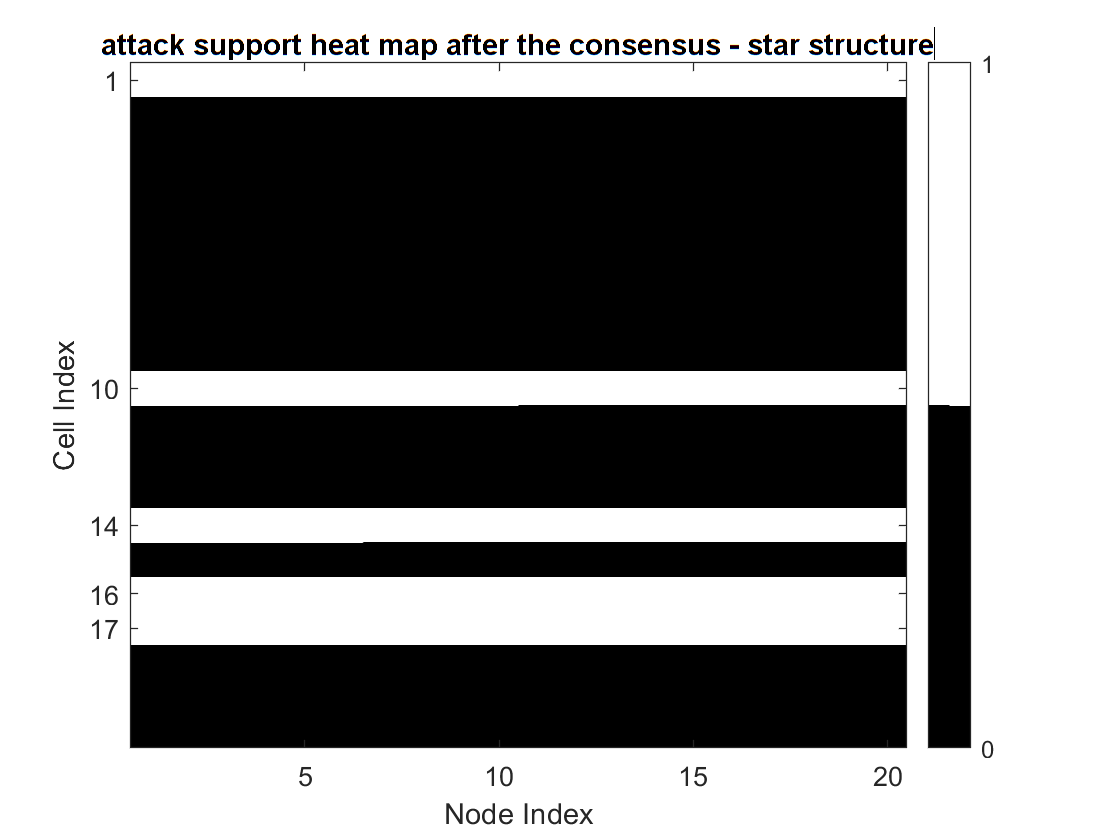
\includegraphics[width=0.45\textwidth]{attack-star.png} % Adjust width as needed
    }
    \caption{Comparison of state and attack support vectors after consensus in the Star topology.}
\end{figure}

In terms of the number of iteration to reahing consensus, both topologies reach consensus in the same order of magnitude; however, ring topology reaches consensus a bit faster. The number of iterations to reach consensus with suggested and enhance parameters can be seen in the following figure.
\begin{figure}[H] % h means "here", can also use t (top), b (bottom), p (page)
    \centering
    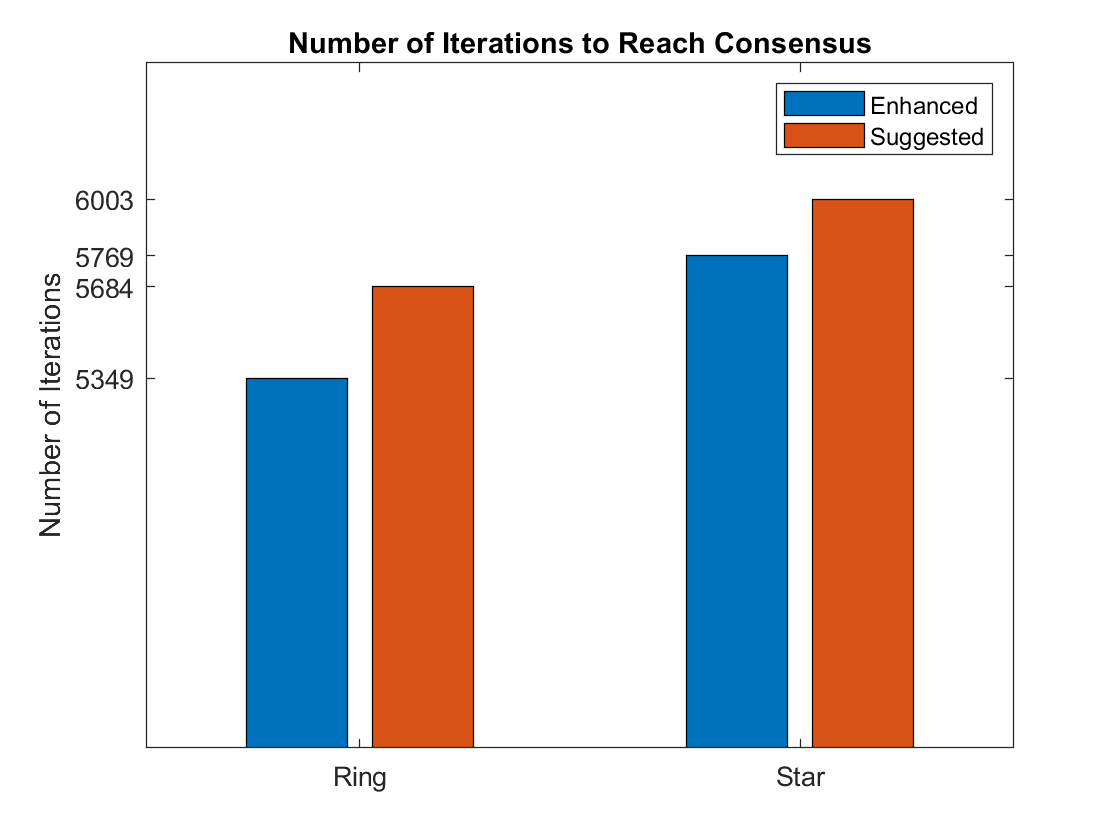
\includegraphics[width=0.45\textwidth]{iteration.png} % Adjust width as needed
    \caption{The number of iterations to reach consensus.}
\end{figure}

A distributed IJAM algorithm may not work well for states with sparse values, due to the fact that this algorithm does enjoy a smooth transient for state estimation, and when a soft-thresholding is applied to the term including the state, the network may not reach a consensus or it may take a large amount of iterations to reach so.

\section{Further discussion}
Consdering the tracking problem the estimation can be enhanced in the following way: after a node realized that its sensor is under attack, it can cutoff the term updating its update based on its measurement, and continue with making the average of the other states, until the sensor reaches a consensus. Therefore, after the attacked nodes stop taking into considerations their measurement, the problem changes to the following format:

\begin{equation}
\min_{x^{(1)}, \dots, x^{(q)}} 
\sum_{i=1,\:\: i\neq\text{attacked sensors}}^q \left\| C x^{(i)} + a^{(i)} - y^{(i)} \right\|_2^2
+ \lambda_1 \sum_{i=1}^q \left\| x^{(i)} \right\|_1
+ \lambda_2 \sum_{i=1}^q \left\| a^{(i)} \right\|_1
+ \frac{\lambda}{2} \sum_{i,j \in \mathcal{N}(i)} \left\| x^{(i)} - x^{(j)} \right\|_2^2
\end{equation}


Since the node keeps on performing averaging, the consensus in the network is going to be guaranteed. Further, since the only measurements that remain are attack-free measurement, the estimation is expected to be more accurate.


\section{Conclusion}
DISTA is capable of providing consensus to the network in both Star and Ring topology. Therefore, all the nodes located the position of the target correctly after the consensus. In addition, they were able to detect the position of the attacked nodes accurately. Ring topology has the advantage that it reaches consensus in smaller number of iteration. 

The reason that IJAM is not used in this process is that it does not enjoy a smooth transient and when soft-thresholding is applied to it, which is the case for this project, the algorithm either the network does not reach a consensu or it reaches in a considerably larger number of iterations.

To enhance the estimation in the tracking problem, once a node detects that its sensor is under attack, it can stop updating based on its own measurement and instead rely on averaging the states of other nodes until consensus is reached. This modifies the optimization problem as follows:

\[
\min_{x^{(1)}, \dots, x^{(q)}} 
\sum_{i=1,\:\: i\neq\text{attacked sensors}}^q \left\| C x^{(i)} + a^{(i)} - y^{(i)} \right\|_2^2
+ \lambda_1 \sum_{i=1}^q \left\| x^{(i)} \right\|_1
+ \lambda_2 \sum_{i=1}^q \left\| a^{(i)} \right\|_1
+ \frac{\lambda}{2} \sum_{i,j \in \mathcal{N}(i)} \left\| x^{(i)} - x^{(j)} \right\|_2^2
\]

By continuously averaging, the network can guarantee consensus. Additionally, since only non-attacked measurements are used, the estimation becomes more accurate.










% !TeX root = ../main.tex
\chapter{Project 06: Distributed Control of a Multi-agent magnetic levitation system}

\section{Objectives}
The aim of this project is analyze the effect of different network structures and control parameters on the cooperative control protocol and the global observer, and finally designing a control protocol and observer to reach consesnsus among the nodes - choosing a network structure among different possible topologies.

\section{Setting of the problem}
\subsection{Dynamics of the Nodes}
The system under study comprises of 7 almost identical magnetic levitation system, of which one is chosen as leader node and others followers. The dynamic of each node is described as follows:


\begin{align*}
\dot{x}_i &= A x_i + B u_i \\
y_i &= C x_i
\end{align*}

with matrices:

\[
A = \begin{bmatrix}
0 & 1 \\
880.87 & 0
\end{bmatrix}, \quad
B = \begin{bmatrix}
0 \\
-9.9453
\end{bmatrix}, \quad
C = \begin{bmatrix}
708.27 & 0
\end{bmatrix}, \quad
D = \begin{bmatrix}
0
\end{bmatrix}
\]

Regarding the observability and controllability of each node, it can be easily investigated that both states of the nodes are observable and controllable. However, as it can be seen only the first state of the system is measured, and an observer, global or local, needs to be used for the perpuse of \textit{State-variable feedback control}. 

The fundamental assumptions regarding the whole system is as follows:
\begin{enumerate}
	\item The leader node $S_0$ can be observed by a small subset of the follower nodes
	\item The controller law of each aget can only enjoy the information of the neighbor nodes
	\item There exists at lead one directed path from the leader node to every follower node.
\end{enumerate}

\subsection{Reference generation by the leader node}
As the nodes are unstable, in order for the leader to generate a reference signal: first, a local observer needs to be adopted for the leader node, and then, a local controller needs to be adopted to perform the eigenvalue placement depending on the desired reference to be generated. For each desired signal, the eigvenvalues of the leader should be placed as follows:
\begin{itemize}
	\item Step reference: [0 , -$\lambda$], with impact input 
	\item Ramp reference: [0, 0], with impact input
	\item Sinusoidal: [+$\omega$j,  -$\omega$j], with impact input
\end{itemize}

In our case, for the sake of conformity of the different tests, these values are chosen as follows:
\begin{itemize}
	\item Step reference: [0 , -5], with impact input 
	\item Ramp reference: [0, 0], with impact input
	\item Sinusoidal: [+j,  -j], with impact input
\end{itemize}

And for the local observer, -10 and -15. In a noise-free case, it is more desirable to choose faster eigenvalue for the observer; this, nonetheless, leads to worsening the performance in an noisy environment, or in the case of using cheap sensors. Therefore, the eigenvalues of the observer should not be chosen to be much large than the eigenvalues of the plant.

Since by the assumption all the nodes need to be identical, the same controller must be used on all the nodes.

The plots of the references generated by the leader are as follows:
\begin{figure}[H] % h means "here", can also use t (top), b (bottom), p (page)
    \centering
    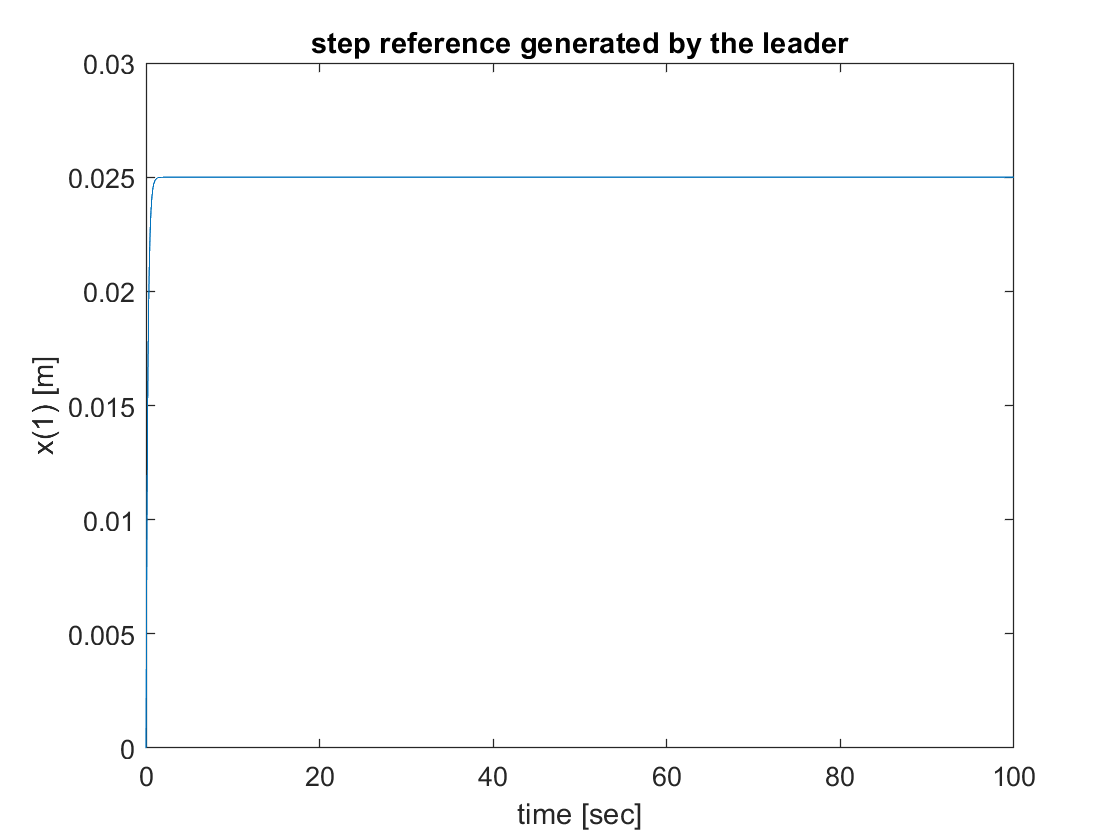
\includegraphics[width=0.55\textwidth]{step_reference.png} % Adjust width as needed
    \caption{Step reference generated by the leader load.}
\end{figure}

\begin{figure}[H] % h means "here", can also use t (top), b (bottom), p (page)
    \centering
    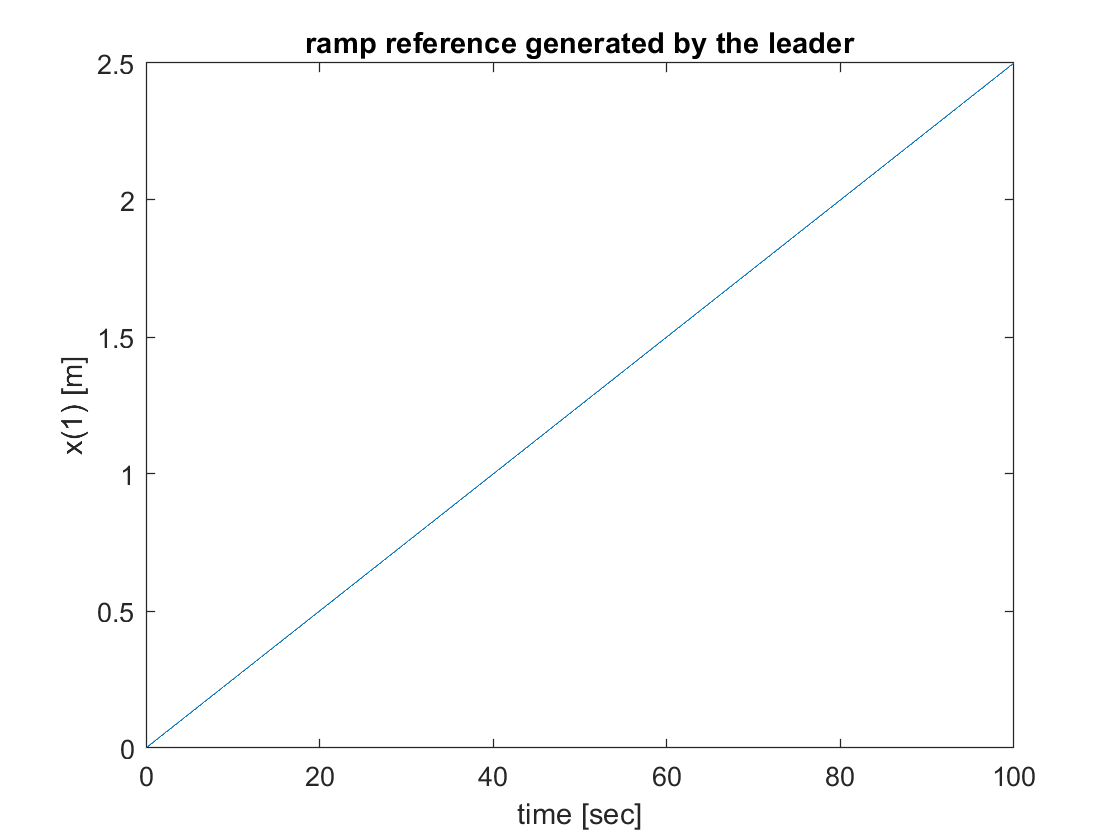
\includegraphics[width=0.55\textwidth]{ramp_reference.png} % Adjust width as needed
    \caption{Ramp reference generated by the leader load.}
\end{figure}

\begin{figure}[H] % h means "here", can also use t (top), b (bottom), p (page)
    \centering
    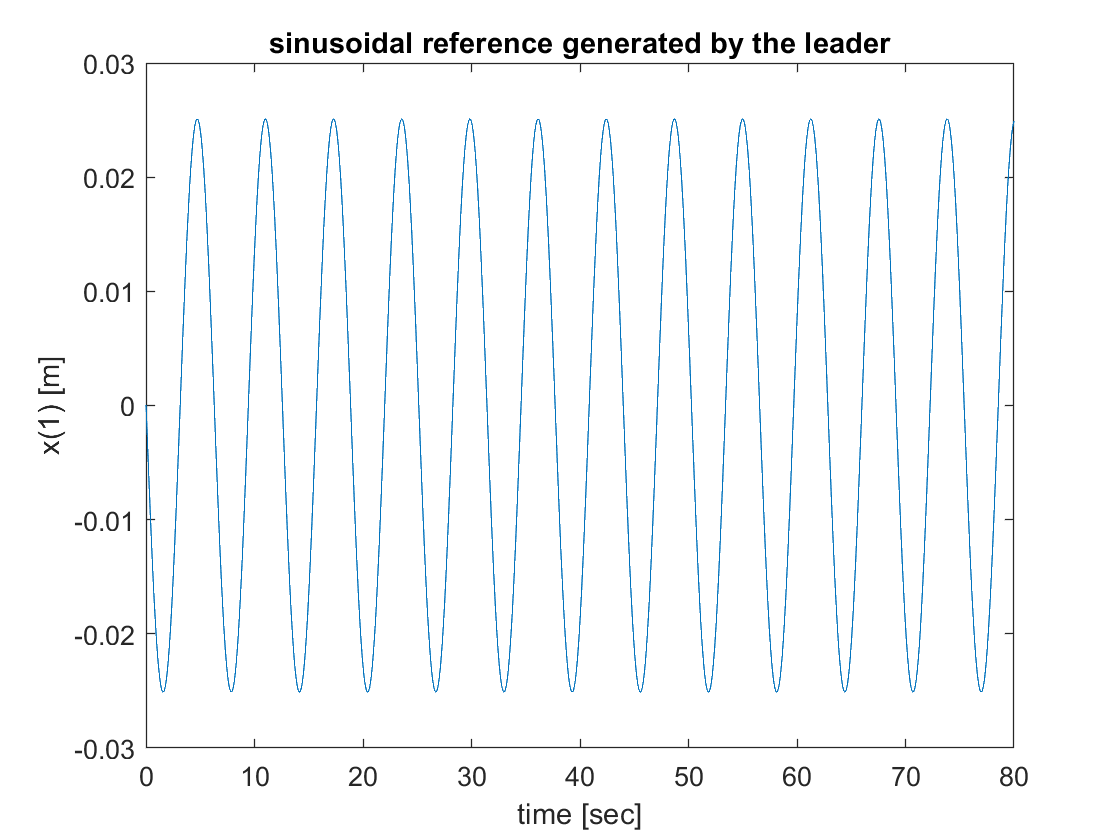
\includegraphics[width=0.55\textwidth]{sinusoildal_reference.png} % Adjust width as needed
    \caption{Sinusoidal reference generated by the leader load.}
\end{figure}


\subsection{Simulation Equation}
For the purpose of simulation, the global dynamics is used, and then the plots are made seperating the relavant states of each nodes. For the case where the local observer are used for the nodes. The state equations used are as follows:


\begin{align*}
A_c &= I_N \otimes A - c_c (L_{\text{cal}} + G_{\text{cal}}) \otimes BK \\
B_c &= c_c (L_{\text{cal}} + G_{\text{cal}}) \otimes BK \\
C_c &= I_{Nn} \\
D_c &= \mathbf{0}_{Nn \times Nn}
\end{align*}

where:
\begin{itemize}
  \item $N$ is the number of agents (excluding the leader),
  \item $n$ is the dimension of the individual agent state (considering the local observer, twice as large as the original $n$),
  \item $A$, $B$ are the agent system modified matrices (the closed-loop node with the controller and the observer),
  \item $K$ is the state feedback gain,
  \item $c_c$ is the coupling gain,
  \item $L_{\text{cal}}$ is the Laplacian matrix of the agent graph,
  \item $G_{\text{cal}}$ is the pinning matrix,
  \item $\otimes$ denotes the Kronecker product.
\end{itemize}

Here, the matrix $C$ is used in this manner so that after the simulation we get all the states of the system.

In case of distributed observer, the following system should be used, where the states vector is the stack of original states and the observer states.

\begin{align*}
A_o &= I_N \otimes A - c_o (L_{\text{cal}} + G_{\text{cal}}) \otimes F C \\
A_c &= 
\begin{bmatrix}
I_N \otimes A & -c_c (L_{\text{cal}} + G_{\text{cal}}) \otimes B K \\
c_o (L_{\text{cal}} + G_{\text{cal}}) \otimes F C & 
A_o - c_c (L_{\text{cal}} + G_{\text{cal}}) \otimes B K
\end{bmatrix} \\
B_c &= 
\begin{bmatrix}
c_c (L_{\text{cal}} + G_{\text{cal}}) \otimes B K \\
c_c (L_{\text{cal}} + G_{\text{cal}}) \otimes B K
\end{bmatrix} \\
C_c &= I_{2Nn} \\
D_c &= \mathbf{0}_{2Nn \times Nn}
\end{align*}

where:
\begin{itemize}
  \item $N$ is the number of agents,
  \item $n$ is the dimension of each agent's state,
  \item $A$, $B$, $C$ are the agent's system matrices,
  \item $K$ is the state feedback gain ,
  \item $F$ is the observer gain,
  \item $c_c$ is the control coupling gain,
  \item $c_o$ is the observer coupling gain,
  \item $L_{\text{cal}}$ is the Laplacian matrix of the communication graph,
  \item $G_{\text{cal}}$ is the pinning matrix,
  \item $\otimes$ denotes the Kronecker product.
\end{itemize}

The controller gain $K$ is obtained by:
\begin{equation} 
K = R^{-1} B^{T} P
\end{equation}
where $P$ is a positive definite solution of the Algebraic Riccati Equation (ARE):
\begin{equation} 
A^{T} P + P A + Q - P B R^{-1} B^{T} P = 0
\end{equation}
and $c_c$ is chosen according to the following criterion:
\begin{equation}
c_c \geq \frac{1}{2 \min\limits_{i \in \mathcal{N}} \operatorname{Re}(\lambda_i)}
\end{equation}

Similarly, the observer gain \( F \) is designed to ensure the estimation error dynamics are stable. Typically, \( F \) is chosen based on the solution \( P \) of the dual Algebraic Riccati Equation:
\begin{equation}
A P + P A^{T} + Q - P C^{T} R^{-1} C P = 0
\end{equation}
The observer gain is then given by:
\begin{equation}
F = P C^{T} R^{-1}
\end{equation}
and the observer coupling gain \( c_o \) is selected by an analogous criterion:
\begin{equation}
c_o \geq \frac{1}{2 \min\limits_{i \in \mathcal{N}} \operatorname{Re}(\lambda_i)}
\end{equation}

Later, the effects of both the coupling gains \( c_c \) and \( c_o \) on system stability and performance will be discussed.

\subsection{Topology of the network}
Among all the possible network topologies, the following topologies are investigated. 
\begin{enumerate}
	\item tree topology
	\item ring topology
	\item fully connected topology with two node connected to the leader
	\item star topology: one node is pinned to the leader
\end{enumerate}

while invesigating the toplogies, all values of adjacancy matrix, pinning matrix are set to 1 so that we investigate only the role of topology.
%%%%%%%%%%%%%%%%%%%%%%%%%%%%
%%%%%%%%%%%%%%%%%%%%%%%%%%%%
%%%%%%%%%%%%%%%%%%%%%%%%%%%%
%%%%%%%%%%%%%%%%%%%%%%%%%%%%
\section{Inverstigating tree topology}
The graph of this topology is as follows:
\begin{figure}[H] % h means "here", can also use t (top), b (bottom), p (page)
    \centering
    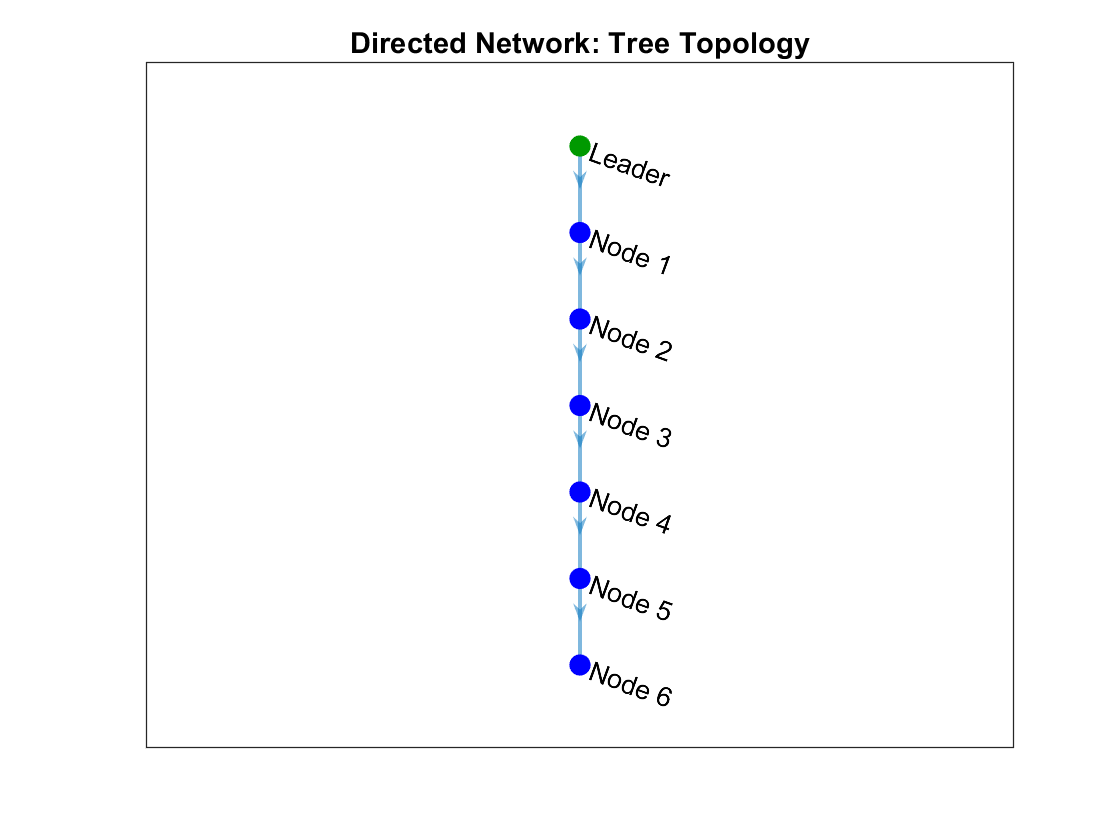
\includegraphics[width=0.50\textwidth]{tree_topology_graph.png} % Adjust width as needed
    \caption{The graph of the communication link in tree topology.}
\end{figure}

\subsection{Distributed control protocol with the local observer}
\subsubsection{Step reference}
\begin{figure}[H] % h means "here", can also use t (top), b (bottom), p (page)
    \centering
    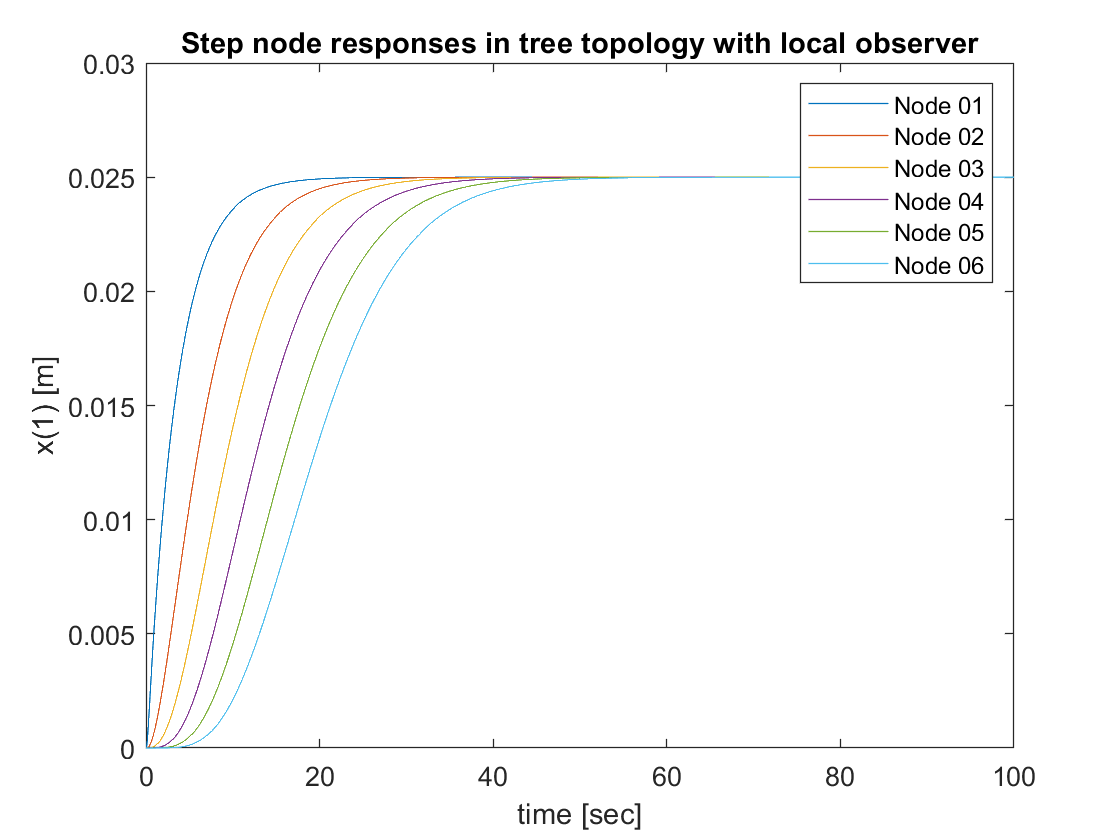
\includegraphics[width=0.50\textwidth]{step_tree_local.png} % Adjust width as needed
    \caption{The response of the nodes with the step reference in tree topology by local observer.}
\end{figure}

\subsubsection{Ramp reference}
\begin{figure}[H] % h means "here", can also use t (top), b (bottom), p (page)
    \centering
    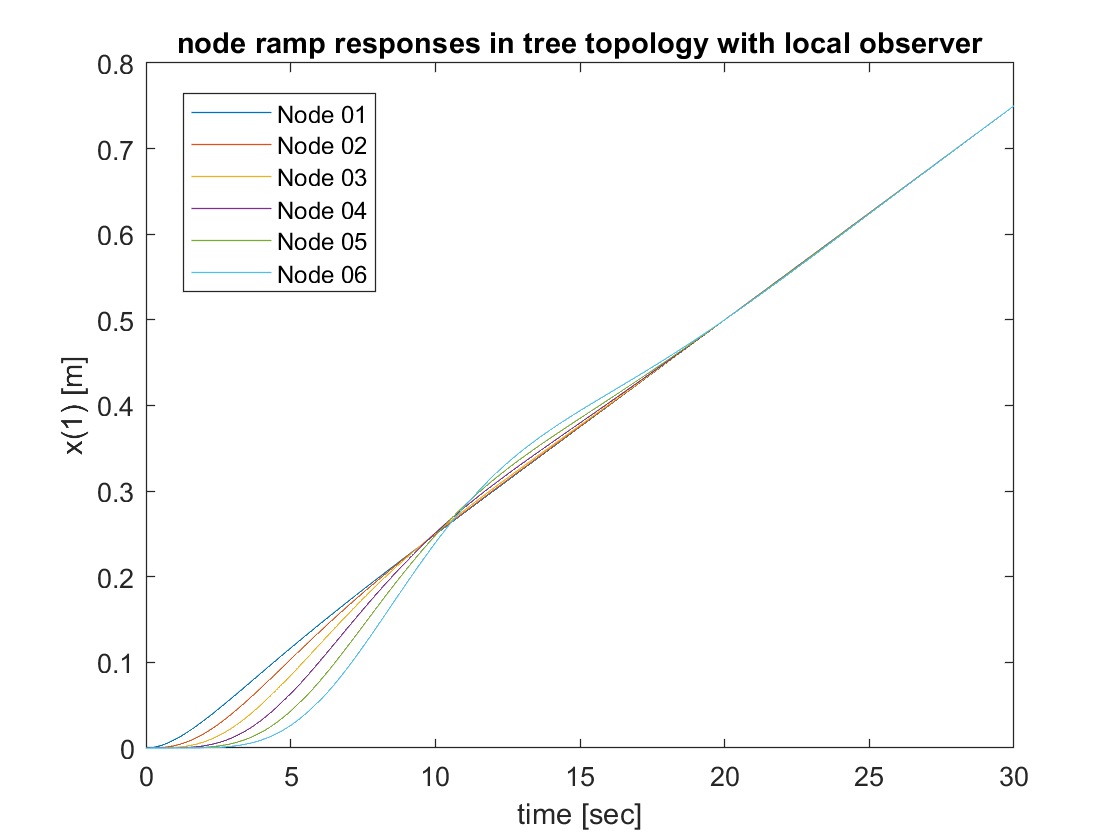
\includegraphics[width=0.50\textwidth]{ramp_tree_local.png} % Adjust width as needed
    \caption{The response of the nodes with the ramp reference in tree topology by local observer.}
\end{figure}


\subsubsection{Sinusoidal reference}
\begin{figure}[H] % h means "here", can also use t (top), b (bottom), p (page)
    \centering
    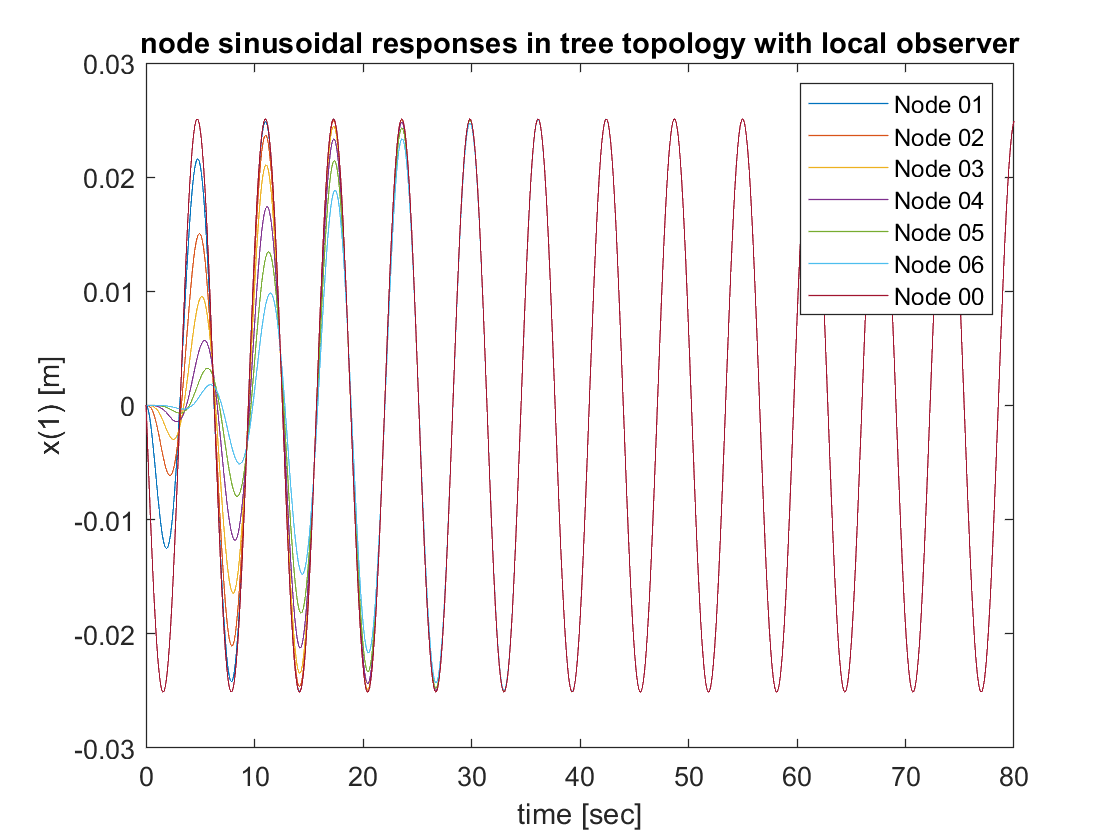
\includegraphics[width=0.50\textwidth]{sin_tree_local.png} % Adjust width as needed
    \caption{The response of the nodes with the sin reference in tree topology by local observer.}
\end{figure}



\subsection{Distributed control protocol with the global observer}
\subsubsection{Step reference}
\begin{figure}[H] % h means "here", can also use t (top), b (bottom), p (page)
    \centering
    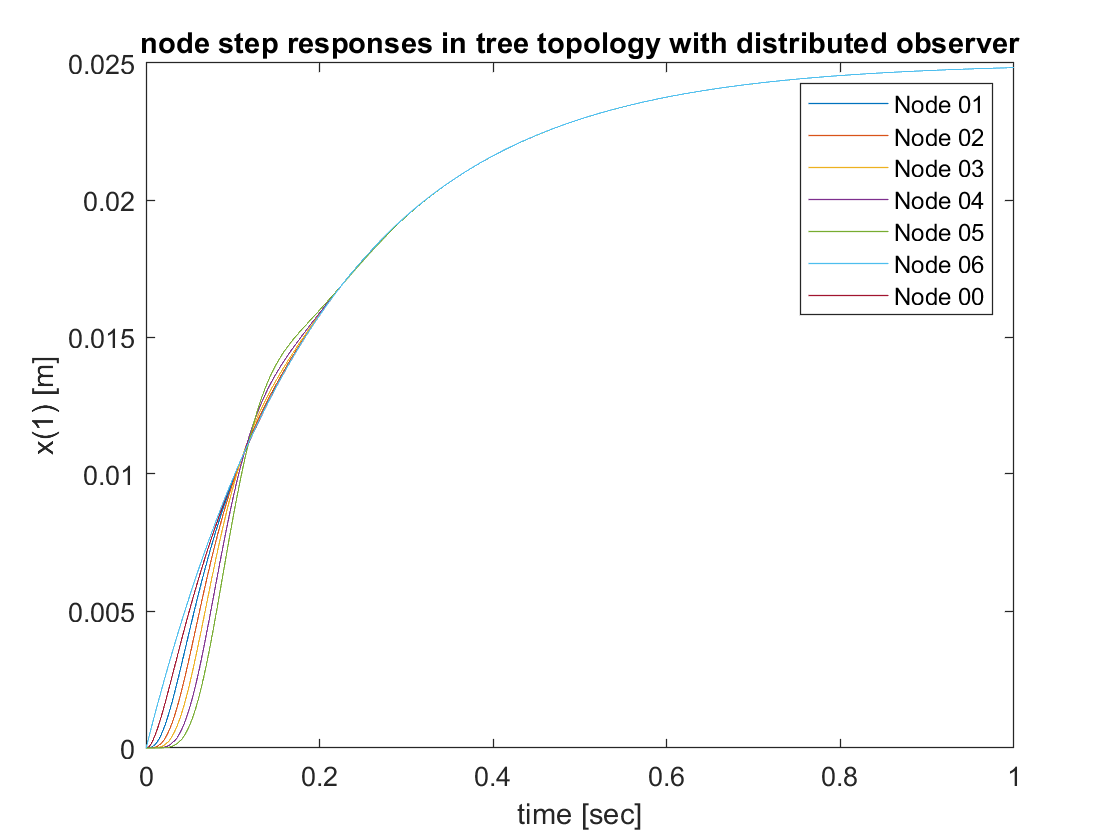
\includegraphics[width=0.50\textwidth]{step_tree_distributed.png} % Adjust width as needed
    \caption{The response of the nodes with the step reference in tree topology by global observer.}
\end{figure}

\subsubsection{Ramp reference}
\begin{figure}[H] % h means "here", can also use t (top), b (bottom), p (page)
    \centering
    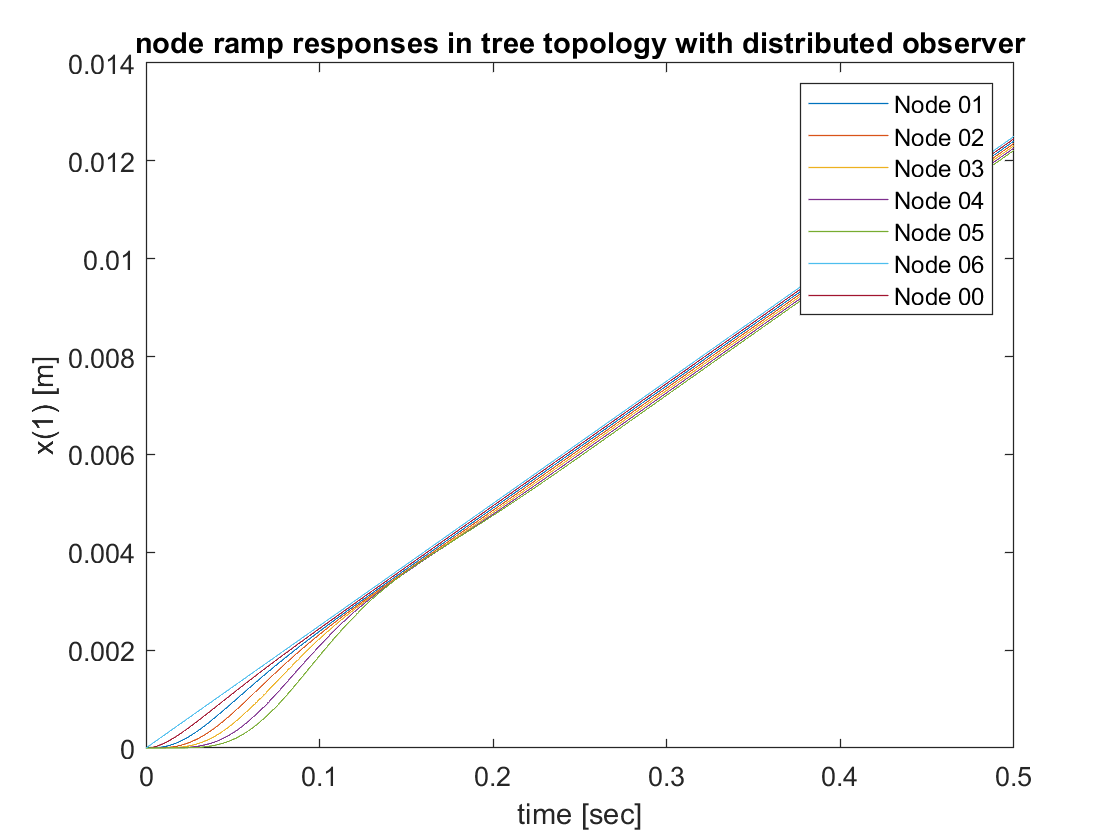
\includegraphics[width=0.50\textwidth]{ramp_tree_distributed.png} % Adjust width as needed
    \caption{The response of the nodes with the ramp reference in tree topology by global observer.}
\end{figure}


\subsubsection{Sinusoidal reference}
\begin{figure}[H] % h means "here", can also use t (top), b (bottom), p (page)
    \centering
    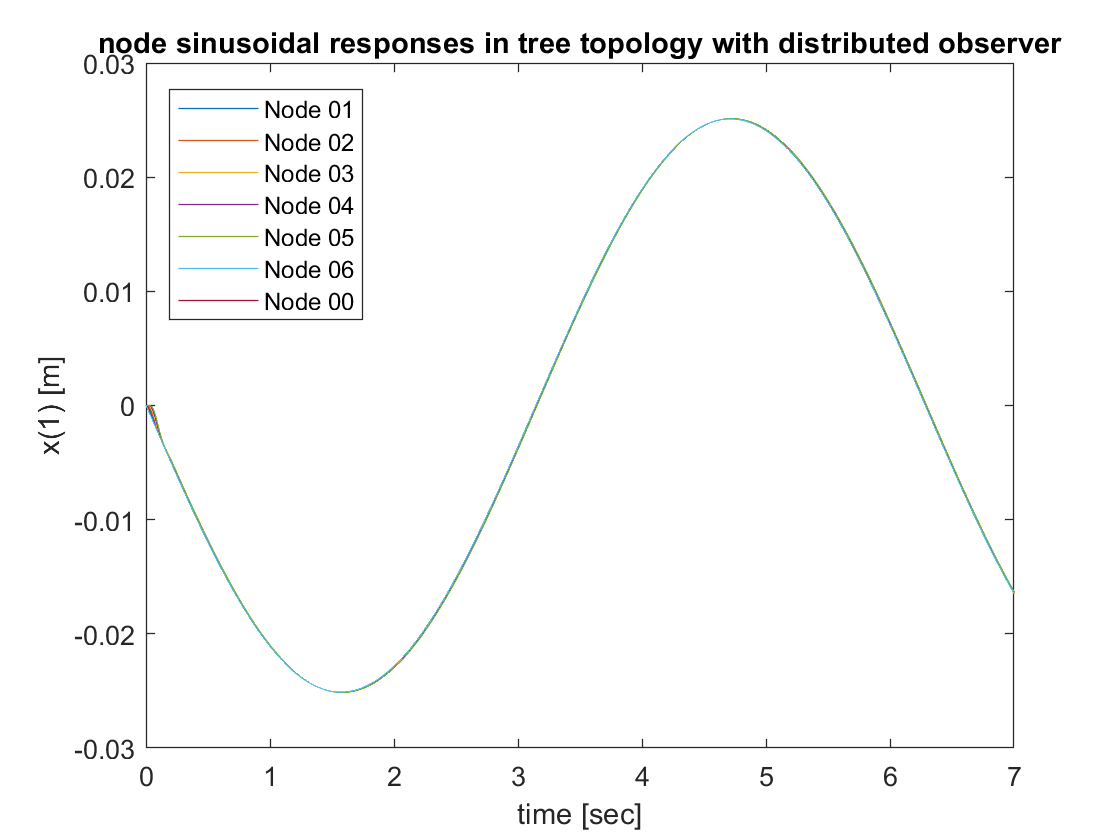
\includegraphics[width=0.50\textwidth]{sin_tree_distributed.png} % Adjust width as needed
    \caption{The response of the nodes with the sin reference in tree topology by global observer.}
\end{figure}


%%%%%%%%%%%%%%%%%%%%%%%%%%%%
%%%%%%%%%%%%%%%%%%%%%%%%%%%%
%%%%%%%%%%%%%%%%%%%%%%%%%%%%
%%%%%%%%%%%%%%%%%%%%%%%%%%%%
\subsection{Investigating Ring Topology}
The graph of this topology is as follows:
\begin{figure}[H] % h means "here", can also use t (top), b (bottom), p (page)
    \centering
    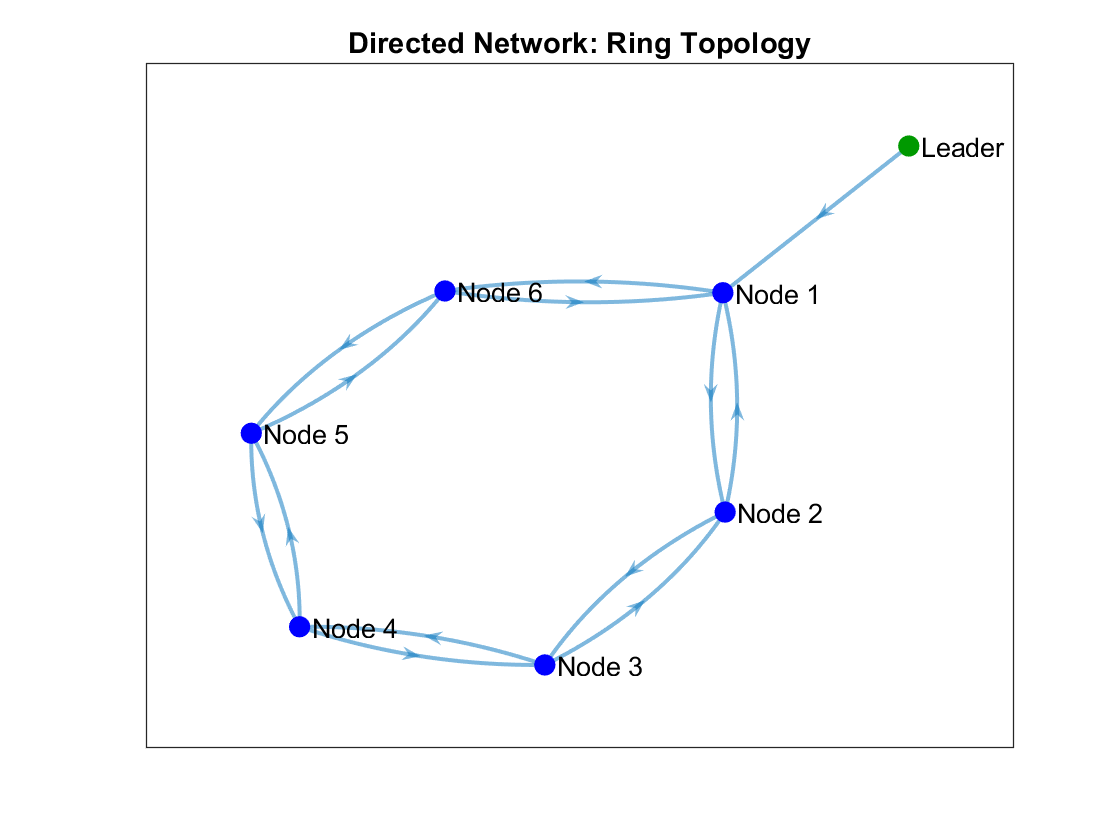
\includegraphics[width=0.55\textwidth]{ring_topology_graph.png} % Adjust width as needed
    \caption{The graph of the communication link in ring topology.}
\end{figure}

\subsection{Distributed control protocol with the local observer}
\subsubsection{Step reference}
\begin{figure}[H] % h means "here", can also use t (top), b (bottom), p (page)
    \centering
    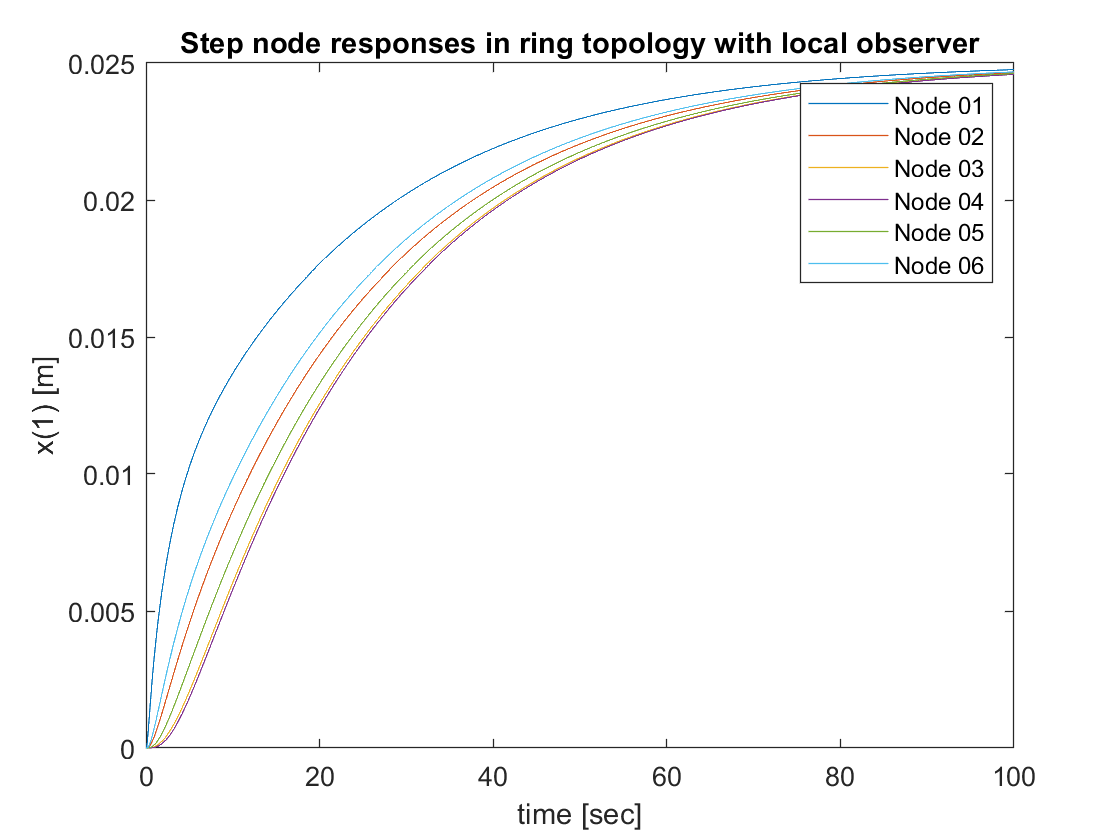
\includegraphics[width=0.50\textwidth]{step_ring_local.png} % Adjust width as needed
    \caption{The response of the nodes with the step reference in ring topology by local observer.}
\end{figure}

\subsubsection{Ramp reference}
\begin{figure}[H] % h means "here", can also use t (top), b (bottom), p (page)
    \centering
    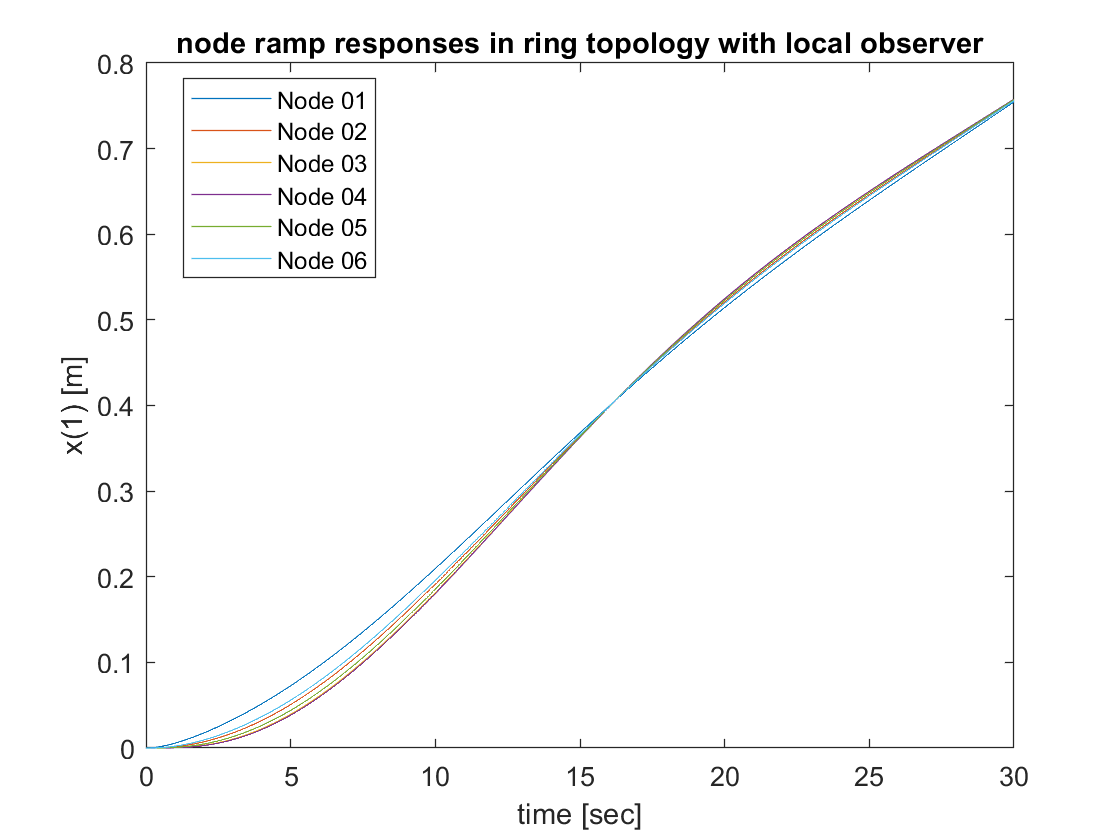
\includegraphics[width=0.50\textwidth]{ramp_ring_local.png} % Adjust width as needed
    \caption{The response of the nodes with the ramp reference in ring topology by local observer.}
\end{figure}

\subsubsection{Sinusoidal reference}
\begin{figure}[H] % h means "here", can also use t (top), b (bottom), p (page)
    \centering
    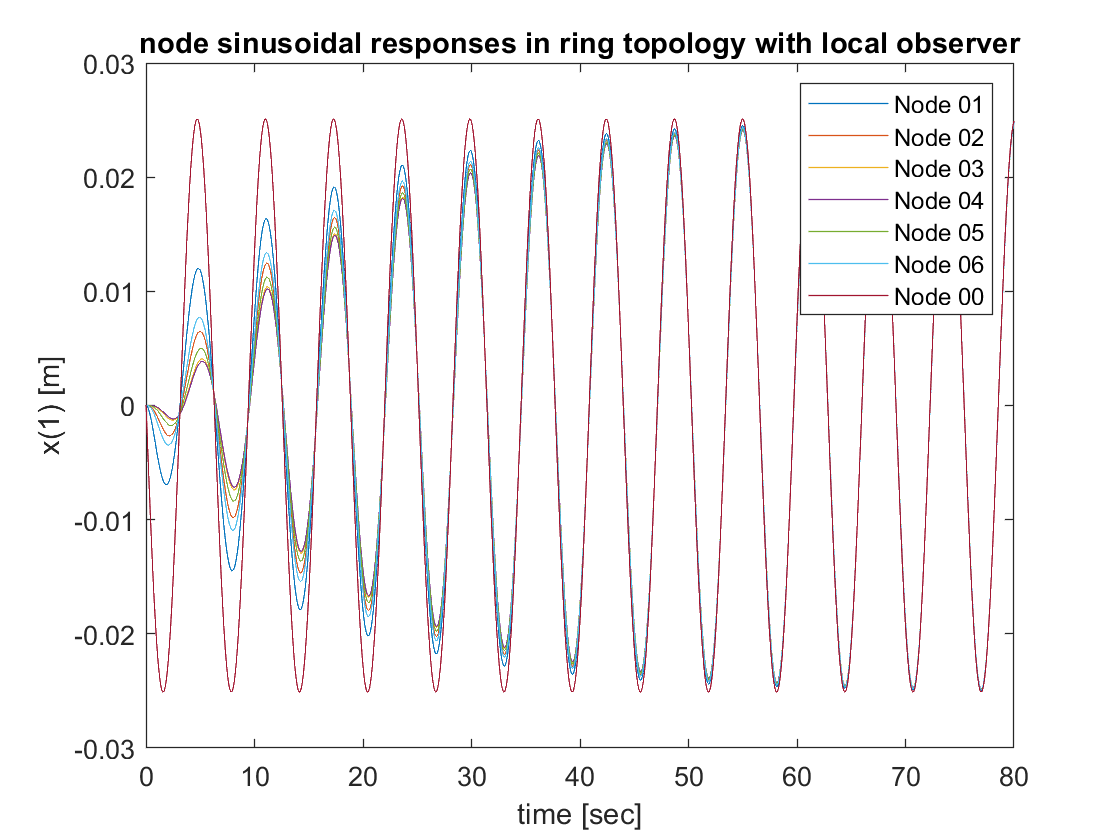
\includegraphics[width=0.50\textwidth]{sin_ring_local.png} % Adjust width as needed
    \caption{The response of the nodes with the sinusoidal reference in ring topology by local observer.}
\end{figure}



\subsection{Distributed control protocol with the global observer}
\subsubsection{Step reference}
\begin{figure}[H] % h means "here", can also use t (top), b (bottom), p (page)
    \centering
    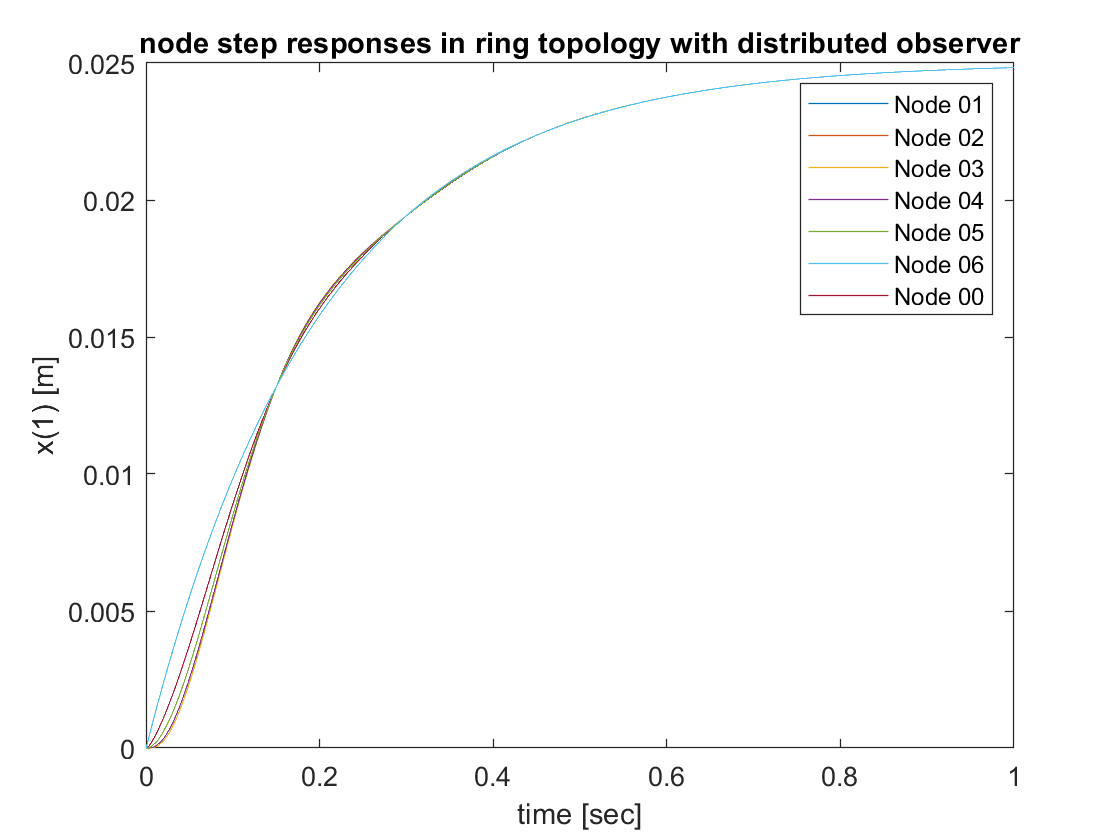
\includegraphics[width=0.50\textwidth]{step_ring_distributed.png} % Adjust width as needed
    \caption{The response of the nodes with the step reference in ring topology by global observer.}
\end{figure}

\subsubsection{Ramp reference}
\begin{figure}[H] % h means "here", can also use t (top), b (bottom), p (page)
    \centering
    \includegraphics[width=0.50\textwidth]{ramp_ring_distributed.png} % Adjust width as needed
    \caption{The response of the nodes with the ramp reference in ring topology by global observer.}
\end{figure}

\subsubsection{Sinusoidal reference}
\begin{figure}[H] % h means "here", can also use t (top), b (bottom), p (page)
    \centering
    \includegraphics[width=0.50\textwidth]{sin_ring_distributed.png} % Adjust width as needed
    \caption{The response of the nodes with the sinusoidal reference in ring topology by global observer.}
\end{figure}

%%%%%%%%%%%%%%%%%%%%%%%%%%%%
%%%%%%%%%%%%%%%%%%%%%%%%%%%%
%%%%%%%%%%%%%%%%%%%%%%%%%%%%
%%%%%%%%%%%%%%%%%%%%%%%%%%%%
\subsection{Investigating fully connected Topology}
The graph of this topology is as follows:
\begin{figure}[H] % h means "here", can also use t (top), b (bottom), p (page)
    \centering
    \includegraphics[width=0.55\textwidth]{full_topology_graph.png} % Adjust width as needed
    \caption{The graph of the communication link in fully connected topology.}
\end{figure}

\subsection{Distributed control protocol with the local observer}
\subsubsection{Step reference}
\begin{figure}[H] % h means "here", can also use t (top), b (bottom), p (page)
    \centering
    \includegraphics[width=0.50\textwidth]{step_full_local.png} % Adjust width as needed
    \caption{The response of the nodes with the step reference in fully connected topology by local observer.}
\end{figure}


\subsubsection{Ramp reference}
\begin{figure}[H] % h means "here", can also use t (top), b (bottom), p (page)
    \centering
    \includegraphics[width=0.50\textwidth]{ramp_full_local.png} % Adjust width as needed
    \caption{The response of the nodes with the ramp reference in fully connected topology by local observer.}
\end{figure}

\subsubsection{Sinusoidal reference}
\begin{figure}[H] % h means "here", can also use t (top), b (bottom), p (page)
    \centering
    \includegraphics[width=0.50\textwidth]{sin_full_local.png} % Adjust width as needed
    \caption{The response of the nodes with the sinusoidal reference in fully connected topology by local observer.}
\end{figure}

\subsection{Distributed control protocol with the global observer}
\subsubsection{Step reference}
\begin{figure}[H] % h means "here", can also use t (top), b (bottom), p (page)
    \centering
    \includegraphics[width=0.50\textwidth]{step_full_distributed.png} % Adjust width as needed
    \caption{The response of the nodes with the step reference in fully connected topology by global observer.}
\end{figure}


\subsubsection{Ramp reference}
\begin{figure}[H] % h means "here", can also use t (top), b (bottom), p (page)
    \centering
    \includegraphics[width=0.50\textwidth]{ramp_full_distributed.png} % Adjust width as needed
    \caption{The response of the nodes with the ramp reference in fully connected topology by global observer.}
\end{figure}

\subsubsection{Sinusoidal reference}
\begin{figure}[H] % h means "here", can also use t (top), b (bottom), p (page)
    \centering
    \includegraphics[width=0.50\textwidth]{sin_full_distributed.png} % Adjust width as needed
    \caption{The response of the nodes with the sinusoidal reference in fully connected topology by global observer.}
\end{figure}


%%%%%%%%%%%%%%%%%%%%%%%%%%%%
%%%%%%%%%%%%%%%%%%%%%%%%%%%%
%%%%%%%%%%%%%%%%%%%%%%%%%%%%
%%%%%%%%%%%%%%%%%%%%%%%%%%%%
\subsection{Investigating star Topology}
The graph of this topology is as follows:
\begin{figure}[H] % h means "here", can also use t (top), b (bottom), p (page)
    \centering
    \includegraphics[width=0.75\textwidth]{star_topology_graph.png} % Adjust width as needed
    \caption{The graph of the communication link in star topology.}
\end{figure}

\subsection{Distributed control protocol with the local observer}
\subsubsection{Step reference}
\begin{figure}[H] % h means "here", can also use t (top), b (bottom), p (page)
    \centering
    \includegraphics[width=0.50\textwidth]{step_star_local.png} % Adjust width as needed
    \caption{The response of the nodes with the step reference in star topology by local observer.}
\end{figure}
In this case, again it can be observed that the rising time is not as fast as the other nodes. It is true that  the lag among the nodes is not as small as fully connected network; nevertheless, the gap is not that much considerable with respect to tree and ring.

\subsubsection{Ramp reference}
\begin{figure}[H] % h means "here", can also use t (top), b (bottom), p (page)
    \centering
    \includegraphics[width=0.50\textwidth]{ramp_star_local.png} % Adjust width as needed
    \caption{The response of the nodes with the ramp reference in star topology by local observer.}
\end{figure}

\subsubsection{Sinusoidal reference}
\begin{figure}[H] % h means "here", can also use t (top), b (bottom), p (page)
    \centering
    \includegraphics[width=0.50\textwidth]{sin_star_local.png} % Adjust width as needed
    \caption{The response of the nodes with the sinusoidal reference in star topology by local observer.}
\end{figure}

\subsection{Distributed control protocol with the global observer}
\subsubsection{Step reference}
\begin{figure}[H] % h means "here", can also use t (top), b (bottom), p (page)
    \centering
    \includegraphics[width=0.50\textwidth]{step_star_distributed.png} % Adjust width as needed
    \caption{The response of the nodes with the step reference in star topology by global observer.}
\end{figure}
In this case, again it can be observed that the rising time is not as fast as the other nodes. It is true that  the lag among the nodes is not as small as fully connected network; nevertheless, the gap is not that much considerable with respect to tree and ring.

\subsubsection{Ramp reference}
\begin{figure}[H] % h means "here", can also use t (top), b (bottom), p (page)
    \centering
    \includegraphics[width=0.50\textwidth]{ramp_star_distributed.png} % Adjust width as needed
    \caption{The response of the nodes with the ramp reference in star topology by global observer.}
\end{figure}

\subsubsection{Sinusoidal reference}
\begin{figure}[H] % h means "here", can also use t (top), b (bottom), p (page)
    \centering
    \includegraphics[width=0.50\textwidth]{sin_star_distributed.png} % Adjust width as needed
    \caption{The response of the nodes with the sinusoidal reference in star topology by global observer.}
\end{figure}

\subsection{Comparing the performance of the difference topologies}
Regarding the performance, it can be seen that the fully connected graph, outperforms other topologies regardless of the reference to be track; nonetheless, in practice this structure includes a lot of communications, and thereby the change of packet loss increases. All in all, taking into account practical considerations and the performance, it can be observed that star topology shows a remarkable performance. Further, in practice a round-robin algorithm can be implemented for the communication of thet nodes with the center node.

\subsection{Comparing the performance of the local observer vs. global observer}
It can be seen that global observer has a really good performance, and in the case that a global observer is used a considerablly faster convergence time is obtained. Therefore, at least in simulation, without any doubt, the global observer outperform the local observer. However, as it can be seen in the following section, the discrete-time version of global observer does not have a satisfying performance.



\section{discretized implementation global observer}
Although in the continuous simulation global observers performs really well, it can be seen that in the discretized implementation of this version, the realize time performance does not show a really suitable transient behavior. Further this performance deteriorates as the sampling time decreases. Another observation is that, in the discrete-time version, the sampling time should match the coupling gain; the larger the coupling gain, the smaller should be sampling time.

The performance of the discrete-time global observer with different sampling times can be seen hereunder.
\begin{figure}[H] % h means "here", can also use t (top), b (bottom), p (page)
    \centering
    \includegraphics[width=0.50\textwidth]{tree_0.001.png} % Adjust width as needed
    \caption{The response of the nodes with the step reference in tree topology by discretized global observer with sampling time 0.001 second.}
\end{figure}

\begin{figure}[H] % h means "here", can also use t (top), b (bottom), p (page)
    \centering
    \includegraphics[width=0.50\textwidth]{tree_0.01.png} % Adjust width as needed
    \caption{The response of the nodes with the step reference in tree topology by discretized global observer with sampling time 0.01 second.}
\end{figure}

\begin{figure}[H] % h means "here", can also use t (top), b (bottom), p (page)
    \centering
    \includegraphics[width=0.50\textwidth]{tree_0.5.png} % Adjust width as needed
    \caption{The response of the nodes with the step reference in tree topology by discretized global observer with sampling time 0.5 second.}
\end{figure}



\section{The effect of the coupling gain $c$ and weight matrices $Q$ and $R$}
It can be seen that by increasing the coupling gain way larger than the threshold recommended by the theory, a better performance is obtained. In practice, nevertheless, it must be considered that using a large coupling gain is accompanied by large control input in the nodes, which depending on the size of the actuator, for relatively large values of coupling gain, saturation may be caused.

$Q$ is a diagonal matrix and it includes the weight of the states. By allocating weights to the states, it can be specified that which state is of higher importance for us.  $R$ is a diagonal matrix, and it include the weigh of the inputs. By increasing the value of $R$, the optimizer finds a solution that reduces the input effort as much as possible. 

It must be taken into account that improving performance is in conflict with reducing the input effort, and therefore, tunning these matrices is a matter of trade-off between these two objectives.


\section{Effect of noise}
Having investigated the effect of noise, it was realized that by increasing the coupling gain, the bound of the noise on the both states reduces, and this is correct also for the measurement noise. However, it seems counter intuitive, since it is expected that by increasing the value of the gain the effect of the noise accentuates.

\begin{figure}[H] % h means "here", can also use t (top), b (bottom), p (page)
    \centering
    \includegraphics[width=0.50\textwidth]{noise1.png} % Adjust width as needed
    \caption{The simulation with noise;theoretical coupling gain plus one}
\end{figure}

\begin{figure}[H] % h means "here", can also use t (top), b (bottom), p (page)
    \centering
    \includegraphics[width=0.50\textwidth]{noise100.png} % Adjust width as needed
    \caption{The simulation with noise;theoretical coupling gain plus one}
\end{figure}




%%%%%%%%%%%%

\section{Selected structure}
Since the nodes are originally unstable, and in practice, the communication between the noddes might not be idea, a local observer is prefered to guarantee the stability of the nodes under any communication channel condition. Further, given the suitable performance of star topology, a star topology is prefered to be used among the follower nodes.


% ---------------------------------------------------------------------
% ---------------------------------------------------------------------
% ---------------------------------------------------------------------

% Declare appendix and set the equation counter format to (A.section.eqNumber)
\appendix
\renewcommand{\theequation}{\thesection.\arabic{equation}}
\input{chapters/Appendix}

\end{document}
